\documentclass{ppgmus}
\usepackage{textcomp}
\usepackage{kchicago}
\interfootnotelinepenalty=10000
\clubpenalty=10000
\widowpenalty=10000

\newcommand{\pd}{PD}
\newcommand{\objeto}[1]{[#1\texttildelow]}

%% newcommand e uma macro local

\autorbib{Figueiró, Cristiano Severo}
\titulo{SinCoPA- Sistema Interativo de Composição,Performance e Análise - Técnicas, Reflexões e Poéticas}
\autor{Cristiano Severo Figueiró}
\ano{2010}
\tipo{doutorado}
\area{Composição}
\lugar{Salvador}
\orientador{Prof. Dr. Pedro Ribeiro Kröger Jr.}
\mes{Maio}

%\cutter{S192}
%% Palavras-chave com termos da biblioteca nacional
%%\chavei{Composição (Música) --- Programas de computador}
%%\chaveii{Música --- Análise, apreciação}
%% Para funcionar em qualquer ppgmus.cls
%%\chaveiii{}
%%\chaveiv{}

%% Palavras-chave corretas
% \chavei{Composição musical}
% \chaveii{Contornos musicais}
% \chaveiii{Quinteto de sopros}
% \chaveiv{Computação musical}
%\cdu{78.02}
%\cdd{781.3}

%\dataDefesa{Salvador}
%\localDefesa{28 de novembro de 2008}

%\figuraTermo{termo-de-aprovacao}
%\escala{.2}

% \bancaiNome{Pedro Ribeiro Kröger Júnior}
% \bancaiTitulo{Doutor em Composição}
% \bancaiEstudo{Universidade Federal da Bahia (UFBA)}
% \bancaiAtuacao{Universidade Federal da Bahia}

% \bancaiiNome{Jamary Oliveira}
% \bancaiiTitulo{Doutor em Composição}
% \bancaiiEstudo{\textit{University of Texas at Austin}, EUA}
% \bancaiiAtuacao{Universidade Federal da Bahia}

% \bancaiiiNome{Liduino José Pitombeira de Oliveira}
% \bancaiiiTitulo{Doutor em Composição}
% \bancaiiiEstudo{\textit{Louisiana State University System}, EUA}
% \bancaiiiAtuacao{Universidade Federal da Paraíba}


%\titulofonte{Qualificativo}
\begin{document}
 


\capa
\begin{dadosTese}
Texto entregue como requisito parcial para Processo Qualificativo de doutorado.
\end{dadosTese}


\title{Qualificativo}
\author{Cristiano Figueiró}



\tableofcontents

\newpage

% \begin{abstract}
%  
% A criação de música interativa é uma tarefa que envolve diversos 
% conhecimentos como técnicas de composição musical, síntese sonora,
% análise e processamento de sinal digital e design de interface.
% Nos últimos anos, diversos projetos vem sendo desenvolvidos e adotados
% pela comunidade de compositores interessados em compôr música baseada
% na interação homem-máquina. Notadamente a linguagem Pure data (Pd),
% vem sendo amplamente adotada pela flexibilidade de extensão de objetos 
% e capacidade de se integrar a outras linguagens e soluções existentes
% no campo da computação musical. Pd é uma linguagem gráfica...
% 
% Mesmo possibilitando diversas soluções ao compositor, o Pd exige
% o estudo formal de sua gramática tal qual qualquer linguagem de 
% programação. Muitas das soluções apresentadas pela comunidade
% são específicas e dificilmente adaptáveis a problemas gerais de 
% composição.
% 
% Nesta pesquisa investigamos o problema da criação de uma biblioteca
% de utilitários que realizem a interação entre os conhecimentos necessários
% para criação de música interativa. A criação dessa biblioteca permite
% soluções híbridas interligando diversas outras bibliotecas gerais e
% específicas desenvolvidas pela comunidade. O uso da biblioteca
% propicia ao compositor uma rápida prototipagem em música interativa e 
% integração com outros fluxos de trabalho, ao mesmo tempo em que permite
% um estudo mais aprofundado da linguagem e customização da própria biblioteca
% apresentada aqui.
% 
% 
% 
% \end{abstract} 

\chapter{Introdução}
\label{sec:intro}


Essa pesquisa apresenta a busca por um modelo de composição e
performance de música interativa – evento sonoro gerado a partir da
performance de um músico sobre uma base de programas, materiais
estocados e análise das informações da performance em tempo-real. O
modelo é materializado na forma de um sistema computacional que seja
capaz de extrair informações diversas sobre a performance e
categorizar aspectos da performance musical e interagir com essa performance.


O sistema é construído com a linguagem \textit{Pure Data} (\pd). O Pd é uma linguagem gráfica orientada ao objeto que surgiu
como linguagem voltada para a criação de música eletrônica e nos últimos anos foi-se desenvolvendo inúmeras
bibliotecas de objetos especializados em modelos matemáticos, modelamentos de interface gráfica, diversas 
implementações
em processamento e análise em tempo-real de sinal de áudio, vídeo, rede e hardware. 
A análise dos dados da performance musical é construída usando objetos ``nativos`` e ``externals`` 
discussão que será
aprofundada no capítulo da metodologia. 
Todas as partes do sistema são construídas em Pd, no formato de objetos
modulares. Os objetos criados tem a função de agregar diversos outros objetos e organizar o fluxo de dados
de análise e performance num contexto que possibilite o re-uso em diferentes projetos e contextos de 
criação de música e arte interativa.Também são apresentados três protótipos de uso do sistema. A visão geral do
SInCoPA é a de uma biblioteca de objetos de Pd e sua documentação de uso, e um catálogo de protótipos e projetos
utilizando essa biblioteca que servem como campo de avaliação de possibilidades e experimentação sonora.


Foram usadas diversas bibliotecas externas ao Pd, algumas que são encontradas na distribuição pd-extended
\footnote{pd-extended é uma distribuição do Pd com várias bibliotecas externas já compiladas na maioria dos
sistemas operacionais existentes. É o principal ''fork`` do Pd, e possui versão estável e versão de desenvolvimento.
A história de desenvolvimento do Pd pode ser entendida como uma sequência de Forks levando a diferentes versões 
e estágios de desenvolvimento locais, como JMax, Max-Ircam, DesireData, etc...Essa pesquisa assume como padrão
a versão atual do pd-extended com algumas adições de bibliotecas de objetos feitos em Pd e alguns objetos codados
em C e compilados como objetos de Pd.}, 
e outras contribuições da comunidade de desenvolvedores.

\section{Problemas}

A criação de música interativa é uma tarefa que envolve diversos 
conhecimentos como técnicas de composição musical, síntese sonora,
análise e processamento de sinal digital e design de interface.

Nesta pesquisa investigamos o problema da criação de uma biblioteca
de utilitários que realizem a interação entre os conhecimentos necessários
para criação de música interativa.

Diversos problemas derivam da intersecção entre descrições simbólicas
de composição e estruturação musical como nota, acorde, motivo e 
especificações de síntese sonora como modulação, envelope e formas de onda.
Alguns problemas são conceituais e demandam um universo próprio de 
pesquisa como por exemplo a detecção automática de começo e fim de
frases melódicas. Outros problemas são técnicos e prevêem uma depuração
na programação como por exemplo a sincronia entre as mensagens de controle de parâmetros
e o processamento de blocos de áudio. 

Como outras linguagens abordam esses problemas (aqui citar artigo
que fizemos pra anppom em 2008  e artigo do Miller - Max at seventeen)


\section{Referências}

Alguns projetos relacionados podem servir como fonte de inspiração pra
a presente pesquisa como o Cypher \cite{rowe93:interactive}   de Rowe que usa a metáfora da
sociedade da mente de Minsky na forma de músicos artificiais dentro de
um sistema multi-agente - o Meta-Cypher inclui múltiplos ouvintes e
performers além de um meta-ouvinte.  O Drum Circle \cite{eigenfeld07:drum} é um sistema escrito em Max/MSP e explora o uso de
multi-agentes sobre uma rede local onde cada agente emula um
percussionista improvisando em um grupo de tambores, tendo como
resultante um ritmo evolutivo.

Um dos projetos mais amplos nessa área é o projeto Omax Brothers \cite{assayag06:omax}
desenvolvido no Ircam. Um sistema multi-agente criado para
improvisação musical entre homem-máquina que aprende em tempo-real com
o performer humano. O núcleo da improvisação é baseado em modelamento
de sequência e aprendizado estatístico. O sistema envolve uma
arquitetura híbrida usando dois ambientes populares para composição e
performance, OpenMusic (baseado em Lisp) para modelamento e
programação de alto nível e Max/MSP para a performance do sistema e
processamento de áudio em tempo-real.

Da parte musical diversas peças motivaram o desenvolvimento desse trabalho como as peças
''Jupiter'' e ''En Echo'' de Philippe Manoury para flauta e computador e soprano e computador respectivamente.
Essas músicas foram desenvolvidas em colaboração com Miller Puckette o criador do Max e do Pd. As duas 
peças empregam o uso da técnica de ''Score-follower``, uma técnica que também foi explorada por mim em
meu trabalho de mestrado, na peça ''Enquanto eles riem``(2005) para Clarinete e computador com Max/MSP.

\section{Processo}

O desenvolvimento cronológico dessa pesquisa levou a um primeiro momento de intenso aprendizado
dos detalhes e técnicas de programação com Pd, desenvolvendo materiais didáticos, traduções, e uma
sequência de estudos interativos usados em peças musicais e performances sonoras. Um exemplo pode ser visto
na figura \ref{flauta2007}, onde um Score-follower controla os parâmetros de 
processamento do som da flauta e harmoniza certos trechos da peça de acordo com as notas da flauta.

\begin{figure}[!h]
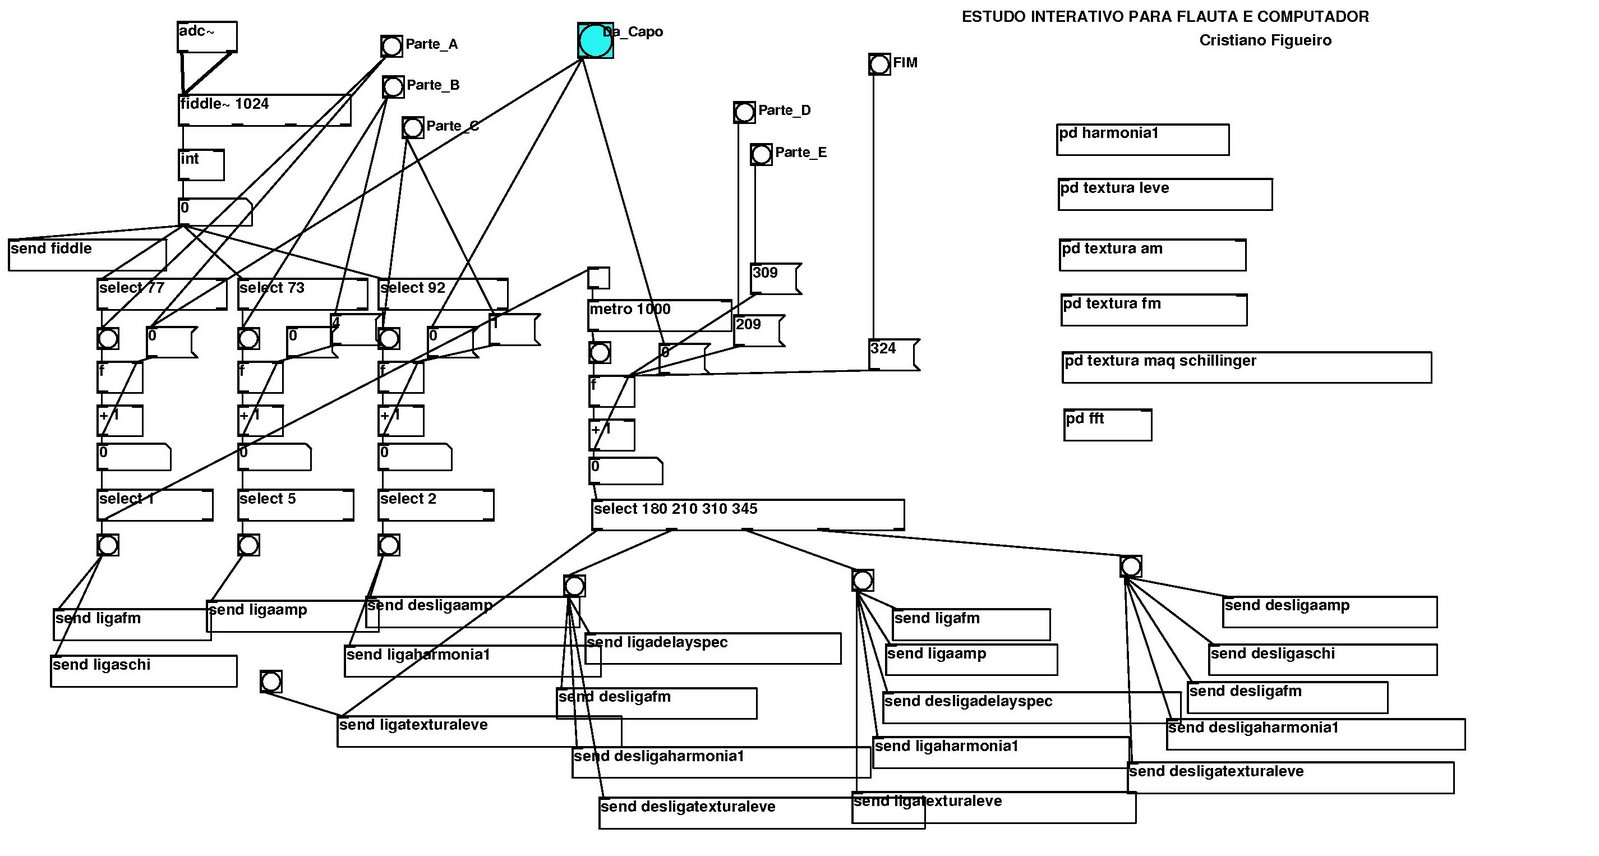
\includegraphics[scale=.3]{flauta2007}
\caption{estudo interativo pra flauta e computador (2007)}
\label{flauta2007}
\end{figure} 

A comunidade de desenvolvimento do Pd é muito ativa, e explicitamente projetos open-source
se esforçam para mudar a condição do interessado no software de usuário passivo a participante ativo do desenvolvimento
e das decisões coletivas sobre os caminhos que a linguagem deve tomar. Esse  fator acarretou na
organização de 2 eventos com desenvolvedores e forte interação com a comunidade\footnote{III International
Convention of Puredata (PdCon) em São Paulo e o I Simpósio Internacional de Interatividade nos Sistemas
Computacionais Livres (wwww.iscl2009.wordpress.com) em Salvador em 2009.}, desenvolvimento de peças interativas para instrumentos
tradicionais e computador, oficinas de extensão, participação em desenvolvimento de projetos coletivos
usando pure data, como navalha e mimosalib usada nos protótipos.



% Pode-se, portanto, definir que uma boa abordagem de pesquisa em sistemas musicais interativos engloba um vasto campo 
% multidisciplinar realizando uma fusão de pesos iguais entre as áeas de psicologia cognitiva, computação e teoria da 
% composição musical.

O desenvolvimento de um sistema dessa natureza envolve um tipo de conhecimento que envolve técnica de
 composição, análise, performance e computação.
 Essa fusão se dá de maneira pragmática, materializada num sistema de software e hardware, capaz de 
responder musicalmente a estímulos musicais e também capaz de aprender e analisar comportamentos musicais do músico tendo 
conhecimento de seu
passado, presente e assim podendo projetar o futuro. A performance desse tipo de situação musical também leva a um  de questões
de como o sistema se comporta em diversas situações de hardware diferentes e qual 
o nível de estabilidade dos aplicativos na prática.



%% ligar esse último parágrafo com o tema dessa introdução

%% parágrafo de conclusão

\chapter{Revisão Bibliográfica}
\label{sec:rev}

O conceito de interação entre uma performance musical e computador vem
sendo definido nas últimas 3 décadas, e possui diferentes nuances de definição
a depender do contexto de idioma e prática musical a que se refere e a tecnologia
em que é implementada. A descrição ''sistemas musicais interativos``, é um
termo introduzido no livro \textit{Interactive Music Systems} 
\cite{rowe93:interactive} e definido como ''sistemas de música 
computacional em que as mudanças de comportamento são responsivas a um
estímulo musical``. Interação em um sentido mais global pode ser definida: 
  ''Interação tem dois aspectos:
tanto as ações do performer afetam a saída do computador, ou as ações do computador
afetam os resultados do performer`` \cite{garnett:2001}.

Isso pode ser comparado a comunicação entre músicos no modelo de  música de 
câmara tradicional onde dois ou mais músicos realizam música escrita, improvisada 
ou mista \cite{winkler93:interactive}.

Em relações interativas mais complexas, ``um compositor pode
delegar vários papéis a um computador num ambiente de música interativa. Ao
computador pode se dar o papel de instrumento, performer, regente, e/ou compositor.
Esses papéis podem existir  simultaneamente e/ou mudar continuamente''\cite{lippe:2002}.



A pesquisa em sistemas musicais interativos vem nos últimos anos
deixando de ser uma abstração teórica e se transformando em realidade
concreta. O corpo de áreas de pesquisa compreende temas como cognição
musical, computação e teoria e análise musical.


Podemos apontar a multi-disciplinaridade dessa pesquisa como pertencente 
ao escopo de uma disciplina genérica emergente denominada Design de Interação(ID).
%%o que é ID
A maioria dos tratados e especificações da ID se referem a interação para a web
e interação homem-máquina focada em paradigmas comerciais. Ainda que essa pesquisa busque
uma maior interação homem-máquina num nível de funcionalidade auxiliar a poética musical, algumas idéias e 
pensamentos da ID podem ser úteis na organização do desenvolvimento do SInCoPA. 
Como por exemplo os sete estágios da ação \cite{norman06:design} onde descreve que para 
descobrir o que torna a
execução de uma tarefa difícil é necessário examinar a
estrutura de uma ação. Ele propõe sete estágios: um para
meta, três para execução e três para avaliação. A seguir cada
estágio será detalhado.
Formalizar a meta – o primeiro estágio refere-se a decisão de
realizar alguma coisa, ou seja, estabelecer a meta a ser
alcançada. A meta é algo a ser atingido, e nem sempre é bem
definida.
Formalizar a intenção – de acordo com Norman as
metas não definem precisamente o que deve ser feito. Para
se transformar em ações as metas precisam ser traduzidas
em definições específicas do que deve ser executado, o autor
denomina essas definições de intenções. As intenções são
ações específicas que foram realizadas para atingir as metas.
Portanto, após determinar a meta a ser alcançada deve-se
determinar quais serão as ações a serem executadas para
atingir a meta estabelecida.
Especificar a ação – após definir as intenções, essas devem
ser traduzidas por um grupo de comandos internos, ou seja,
uma sequência de ações que possam ser desempenhadas de
modo a satisfazer a intenção. Ressalta-se que até esta etapa
tudo ocorre mentalmente.
Executar a ação – com a sequência de ações definidas,
deve-se colocar em prática o que foi estabelecido.
Ter a percepção do estado do mundo – esta fase esta
intimamente relacionada com a posterior (interpretar o estado
do mundo). Neste momento, deve-se perceber as alterações
ocorridas no ambiente que ocorre a ação.
Interpretar o estado do mundo – após a percepção deve-se
analisar e compreender o que ocorreu no ambiente em
questão.

Avaliar o resultado – por fim, deve-se comparar o resultado
obtido com a meta estabelecida para concluir se o que foi
planejado foi de fato alcançado.
Norman deixa claro que estes estágios não são regras,
são apenas um modelo aproximado para compreender como
os indivíduos fazem as coisas. Esses estágios podem facilmente
ser pensados como um método para um design do desenvolvimento 
de um projeto interativo. Apesar da presente pesquisa não usar de 
maneira sistemática esse método, esses estágios pode servir como
método de avaliação ao final do desenvolvimento.

Outra área emergente que possui muitas características em comum com essa
pesquisa é a disciplina que se chama ''Realidade Aumentada`` (RA), que é uma linha de pesquisa dentro da ciência da computação que lida com 
integração do mundo real e elementos virtuais ou dados criados pelo computador. Atualmente, a 
maior parte das pesquisas em RA está ligada ao uso de vídeos transmitidos ao vivo, que são 
digitalmente processados e “ampliados” pela adição de gráficos criados pelo computador.

A definição de Ronald Azuma 
sobre a Realidade Aumentada \cite{azuma97:ar} é uma descrição genérica que pode nos auxiliar na delimitação teórica. 
Ela ignora um subconjunto do objetivo inicial da RA, porém é entendida como uma representação 
de todo o domínio da RA: Realidade Aumentada é um ambiente que envolve tanto realidade virtual 
como elementos do mundo real, criando um ambiente misto em tempo real.
Azuma define a Realidade Aumentada como um sistema que:
\begin{itemize}
 \item combina elementos virtuais com o ambiente real; 
  \item é interativa e tem processamento em tempo real; 
  \item  é concebida em três dimensões.
\end{itemize}

    
Se pensarmos em uma realidade aumentada sonora, chegaremos a uma definição que se afina 
com alguns objetivos dessa proposta.
Um projeto similar nesta busca de interatividade sonora é o RjDj - uma companhia que desenvolve 
software de áudio para IPhone, baseado em Pure data. Cada software 
é chamado "cena" e é feito em Pd. Cada "cena" se ocupa em explorar alguns 
aspectos sonoros do ambiente e interagir responsivamente com esses sons, criando uma 
outra narrativa com elementos reais a volta. A experiência de escutar sua voz distorcida,
somada a outros sons do ambiente sonoro, provoca uma mudança de percepção até então 
explorada somente no circuito da música eletroacústica e experiências de laboratório. 
O RjDj possibilita experiências sonoras únicas, integrando o som do ambiente , 
inventividade sonora e re-combinação através de software. Pode-se considerar o 
RjDj um real experimento em realidade aumentada no campo sonoro, uma vez que uma ''cena``
pode ''harmonizar`` eventos sonoros acontecidos ao redor, ou modificar o andamento de
uma música pelo sensor de movimento do IPhone. Os inventores do RjDj, costumam chamar 
o sistema deles de ''droga digital``, pois é capaz de alterar o estado de percepção sonora,
de acordo com a cena carregada e com os estímulos do ambiente e do usuário. 



A pesquisa em computação musical tradicionalmente se utiliza de
desenvolvimentos em redes neurais artificiais (ann – artificial neural
networks), agentes inteligentes artificiais e outros ramos da pesquisa
em inteligência artificial (IA); a produção musical oferece ótimos
casos - teste para a pesquisa em IA. Esse projeto apresenta o desafio
de construir um sistema que use elementos da pesquisa em IA
possibilitando uma interação próxima com músicos humanos e que seja
uma base de trabalho funcional para a prática artístico-musical. Isso
é mais fácil de falar do que de fazer; as habilidades de músicos
humanos em fluidez de ação, capacidade de resposta a situações novas e
referências culturais, transformam a capacidade de interação dos
sistemas computacionais numa árdua tarefa. O fato do sistema ter como
paradigma a criação de música em tempo-real ainda requere uma grande
dimensionalidade de descrições, rápido aprendizado, respostas e
efetiva capacidade de antecipação. O campo de pesquisa em sistemas
musicais interativos\cite{rowe93:interactive} se consiste em sistemas de software e
hardware criados para o fazer musical, mais tipicamente na performance
de concertos ao vivo combinando máquinas e músicos humanos. Os
trabalhos atuais nesse campo incluem ao mesmo tempo a análise de áudio
em tempo-real, cognição musical e experiências em IA e robótica; um
projeto inspirador nesse campo é o MahaDeviBot \cite{kapur07:integrating}, que
é um robô percussionista armado de treze tambores, capaz de se
sincronizar com um sitarista humano através de sensores.

Segundo a classificação de sistemas musicais interativos \cite{rowe93:interactive}
este é um sistema centrado no paradigma da performance, focando tanto
no instrumento quanto no performer. A classificação de sistemas
musicais interativos de Rowe prevê 3 dimensões de classificação de
sistemas:

\begin{enumerate}
\item Programas dirigidos pela ``partitura'' (score-followers) ou
  dirigidos pela performance (interação pela improvisação);
\item Diferenças em relação ao método de resposta pelo sistema que
  podem ser: transformativos, generativos ou sequenciados.
\item Distinção entre paradigmas de construção do sistema. Podemos
  distinguir entre sistemas com paradigma no instrumento, com a idéia
  de extender virtualmente as capacidades tradicionais dos
  instrumentos gerando estruturas como hyperinstruments, (aqui citar
  Machover e Impett). E finalmente sistemas calcados no paradigma do
  performer que tentam construir músicos artificais, uma presença
  musical com personalidade e comportamento próprios com graus
  diferentes de intervenção e influência do músico humano.
\end{enumerate}

A pesquisa que aqui se apresenta pode se enquadrar como dirigida pela
performance com respostas transformativas e generativas e tendo o
paradigma de construção calcado no performer. Durante o mestrado foram
desenvolvidas composições utilizando um score-follower construído em
Max/MSP. Nesse caso o tipo de interação foi dirigido pela partitura
com respostas sequenciadas e tendo paradigma no performer.
Consideramos esse tipo de interação como um nível médio de interação,
pois apesar do computador executar sozinho, ele sempre executa trechos
pré-estabelecidos. No presente trabalho, iremos considerar como
situação composicional ideal a possibilidade de “ensinar” certos
comportamentos musicais apenas através da performance musical, ou
seja, um ambiente que aprenda dinamicamente padrões de execução e
resposta do músico humano e possa interagir com esses padrões,
reiterando, competindo, negando ou propondo novas situações.

Uma outra classificação derivada da de Rowe, é a apresentada na forma
de ``Técnicas de Interação'' \cite{pestova:tese}, onde  explica:
\begin{quote}
 Um breve exame de técnicas de interação comum e sincronização entre o
performer e o computador em obras com eletrônica ao vivo, e também dos problemas
envolvidos e possíveis soluções da literatura
\end{quote} 

Nesse sentido são apresentadas duas grandes categorias para classificar peças
de música interativa:

\begin{itemize}
 \item Score Following
  \item Score Orientation
\end{itemize}




%* modelos de interação - música de câmara /duo-henrique/nunzio 




Na classificação de sistemas \cite{rowe93:interactive} o trabalho de construção de um sistema interativo se
baseia na transversalidade de  três campos de pesquisa: teoria
musical, AI e ciência cognitiva. A presente pesquisa se inspira e usa
livremente elementos e idéias de pesquisas em teoria musical,
composição e cognição musical. Em relação a representação dos sons
dentro de um contexto de trabalho composicional \cite{xenakis96:determinacy}, aponta o
uso de um espaço multidimensional como auxiliar na representação das
características de um som como um gráfico que auxilie a composição,
ordenando cada característica de um som  como altura, amplitude,
tempo, densidade, desordem, parâmetros de timbre, etc..; onde cada
característica é uma linha uni-dimensional, e os sons, pontos
paralelos em várias dimensões. Assim o trabalho composicional pode ser
visto como distribuir pontos em uma linha, onde podemos trabalhar com
simetria, assimetria, repetição, variação ou surpresa.

Em relação a esta proposta, Xenakis acrescenta: 

\begin{quote}
Tradicionalmente a música tem duas dimensões estabelecidas - tempo e
altura. Historicamente outras foram adicionadas como, por exemplo, as
dinâmicas, ainda que estas tenham sido um tanto vagamente
representadas na música instrumental. Com o desenvolvimento da música
eletrônica e da música computacional, a multidimensionalidade da
representação do som se tornou ao mesmo tempo natural e prática. Mas a
música vai além da multidimensionalidade - ela é ainda mais complexa. \cite{xenakis96:determinacy}
  
\end{quote} 

Com o termo complexidade, ele se refere às correlações entre os níveis
de construção de uma peça musical. Mostra um exemplo rápido de três
níveis em que o nível zero abrange altura, intensidade e timbre. No
nível um, frases e acordes e no nível dois a forma.

Uma das características de um sistema interativo é a capacidade do sistema
de emular técnicas composicionais e responder ``compondo'' em tempo-real a
estímulos musicais provindos de músicos humanos. Para isso deve-se implementar
no sistema técnicas de composição que sejam a maneira como o sistema ``percebe''
e responde aos estímulos. Nesse sentido o conceito de “permeabilidade” de 
alturas \cite{ligeti58:transformacoes} pode ser um conceito muito útil se aplicado aos parâmetros
de análise das alturas pelo sistema. Segundo Ligeti:

\begin{quote}
  A tendência geral conduz, então, para a insensibilização da
  fisionomia dos intervalos. Sucessões de tons e superposições
  verticais tornam-se, em grande escala, indiferentes frente aos
  intervalos dos quais provem; conceitos como consonância e
  dissonância se tornam irrelevantes: tensões e distensões podem ser
  obtidas com qualidades estatísticas da forma, como relação de
  registros, densidade ou tipos de tecido das estruturas [...] A perda
  da sensibilidade perante os intervalos conduz a um estado que
  poderíamos chamar de permeabilidade. Isso significa que estruturas
  de diferentes qualidades que transcorrem simultaneamente podem
  interpenetrar-se e mesmo dissolver-se completamente mudando apenas
  as relações de densidade horizontal e vertical, sendo indiferente,
  em princípio, quais intervalos se cruzam em detalhe [...] Embora a
  permeabilidade não tenha tido, até o momento, nenhuma influência
  decisiva sobre a forma, não era desconhecida nos estilos musicais
  antigos. Quem teve o grau mais baixo de permeabilidade até agora
  talvez tenha sido Palestrina, em cuja música vozes simultâneas,
  reguladas por leis expressas univocamente, enrolavam-se umas na
  outras. As possibilidades de combinações intervalares, fortemente
  fixadas, não permitiam a menor ambigüidade no transcurso das
  estruturas; portanto, as relações entre dissonância e consonância
  estavam tratadas, naquele estilo, com o maior cuidado.
\end{quote}
 
Ligeti fala aqui sobre uma permeabilidade dos intervalos de altura,
pode-se pensar em ampliar, e implementar no sistema, esse pensamento
de permeabilidade para conceitos como permissividade evolutiva,como por
exemplo, a permissividade de emergência de estruturas derivadas do material 
da própria análise do timbre do áudio de entrada. Outro exemplo poderia ser a 
emergência de certos comportamentos contrastantes em trechos isolados do material.
A permeabilidade de alturas pode ser um parâmetro de análise das alturas 
de uma performance em tempo-real. Outra possibilidade de aplicação pode ser o
controle geral da permeabilidade de alturas, tendo o sistema a capacidade de
classificar a porcentagem da permeabilidade envolvida em cada trecho. Segundo
Ligeti: 

\begin{quote}
  A insensibilidade frente aos intervalos e a grande permeabilidade é
  ainda mais importante na música de Cage e seu círculo, proveniente
  de princípios totalmente diferentes. Existem obras de Cage que podem
  ser executadas tanto isoladamente quanto de forma simultânea com
  outras partituras onde, então, cada peça se transforma em capa de
  uma possível superposição que, se bem será mais densa que suas
  componentes, não está composta de forma diferente delas. A
  indiferença de tais estruturas, resultado de manipulações com o
  acaso, está estreitamente relacionada com a indiferença dos produtos
  automáticos da música serial primitiva. Essa indiferença tende
  também, por sobre as relações intervalares, para uma ampliação das
  outras dimensões musicais. Uma vez eliminadas as relações
  hierárquicas, afrouxadas as pulsações métricas simétricas,
  transposto os graus de duração, de intervalos e de timbre das
  distribuições seriais, torna-se cada vez mais difícil controlar os
  contrastes.
\end{quote}

Podemos pensar no conceito de permeabilidade como uma técnica composicional
que pode ser quantificável, portanto passível de ser implementada em um programa
de computador e agregada ao sistema que aqui se propõe. Esse conceito pode ser
aplicável aos outros parâmetros do som e radicalizando esse pensamento podemos
pensar no ato composicional como um controle dinâmico entre diversos níveis de 
permeabilidade em todos parâmetros do som.


Outros conceitos composicionais são passíveis de implementação e portanto úteis 
ao universo de referências composicionais necessários ao sistema. Como por exemplo 
alguns conceitos da Gestalt aplicados a música. A Teoria da Gestalt, em suas análises estruturais, 
descobriu certas leis que regem a
percepção humana das formas, facilitando a compreensão das imagens e idéias. Essas leis são
nada menos que conclusões sobre o comportamento natural do cérebro, quando age no
processo de percepção. Os elementos constitutivos são agrupados de acordo com as
características que possuem entre si, como semelhança, proximidade e outras. O fato de o cérebro agir 
em concordância com os princípios Gestálticos já poderia ser
considerado a evidência fundamental de que a Lei da Pregnância é verdadeira. São estas,
resumidamente, as Leis da Gestalt: semelhança, proximidade, pregnância, boa continuidade, clausura e 
experiência passada.

A reflexão sobre as estruturas sonoras numa performance musical a partir do estudo
da percepção com o olhar da gestalt, pode ajudar o compositor a estruturar um 
discurso interativo. Segundo Schachter:
\begin{quote}
 Com o campo da interação, a percepção deve se tornar mais importante que a tecnologia.
Com isso em mente, estratégias composicionais que incluírem qualquer tipo de software
 para interação deve evitar uma dependência excessiva de plataformas específicas de 
computadores. Ao invés disso, a percepção da unidade da construção e a manipulação de
diferentes níveis de controle em tempo-real e randomicidade ou níveis de organização
aleatória, deve permanecer nas mãos do compositor/performer...Eu gostaria de apontar
três abordagens principais ou referências para essas idéias sobre o discurso baseado
na percepção:
\begin{enumerate}
 \item A idéia do critério perceptual, baseado na teoria da Gestalt, começando com
Max Wertheimer e seguido por Marc Leman.
  \item A nova abordagem em relação a percepção na análise de cena auditiva por Albert
Bregman.
  \item A Tipo-morfologia de Pierre Schaeffer no seu ``Tratado dos objetos musicais'',
e a Espectromorfologia de Denis Smalley no ``A linguagem da Música eletroacústica'', editado
por Simon Emmerson.
\cite{schachter07:discourse}
\end{enumerate}
\end{quote} 


Marc leman introduz um modelo que conecta processamento de 
sinal sonoro musical a análise musical e psicoacústica computacional onde interação
se torna um problema central \cite{leman96:gestalt}. Ele afirma que a percepção não deve ser entendida estáticamente,
sem evolução temporal, mas como uma interação evolutiva entre um organismo e um estímulo.

Uma expansão desse pensamento pode ser visto nos autores da ``neo-Gestalt'' ao considerar
a análise da percepção baseado nos princípios da Gestalt:
\begin{itemize}
 \item Proximidade
  \item Similaridade
  \item Boa continuidade
  \item Encerramento
  \item Destino Comum
\end{itemize}
Essas idéias são extendidas na nova análise considerando-se que existem dois níveis de
resposta ou estágios do processo perceptual.
\begin{itemize}
 \item Automático, instintivo e sem esforço;
  \item Voluntário, aprendido e esforçado;
\end{itemize}


A teoria da Gestalt pode facilmente ser criticada pelo fato de ser baseada na descrição
do processo de percepção e não prover um modelo que explique como se forma ou como é constituída 
a percepção humana. 
Uma possibilidade de pesquisa seria usar as leis da Gestalt para refinar os arquivos de treinamento das redes 
do sistema. Nesse caso o programador calibra os pesos dos dados de análise, que vão ser os arquivos de 
treinamento das redes, de acordo com a descrição gestáltica de sua própria percepção. Alguns outros 
conceitos composicionais podem ser implementados ao sistema como questões de direção, densidade, tensão
 e repouso, acumulação, proporção e relações diversas entre durações e ataques.

Uma referência importante para a organização e análise de material sonoro baseada
na análise do áudio e dos eventos sonoros é a Espectromorfologia exposta por Denis
Smalley. Particularmente os conceitos de \textit{Nível e Foco} e \textit{Textura e Gesto},
investigando sua relação com o processamento ao vivo e com o diálogo interativo entre
instrumentos e sons eletroacústicos.

A idéia de \textit{Nível e Foco} tem a ver com interação e o grau de organização aleatória
ou randômica envolvido. Nesse ponto Smalley diz que ``..à nós precisa ser oferecido
a possibilidade de variar nosso foco perceptual através de um registro de níveis 
durante o processo de escuta..''. Para sobreviver a repetidas audições, uma obra deve 
possuir esse potencial focal. Uma música mista para instrumentos tradicionais e eletroacústica, 
baseada numa estrutura aberta, não deve confiar na habilidade do ouvinte para descobrir
os detalhes pequenos e escondidos da composição. A exploração focal dos níveis estruturais
deve permitir diferentes modos de conectar perceptualmente os materiais sonoros com 
o mesmo discurso sonoro. 

De acordo com as palavras de Smalley \cite{emmersonsimon:86}, ``gesto'' tem a ver 
com trajetória, com a aplicação de energia e suas consequências; e é complementar
a causalidade. Essa idéia de Gesto é central à análise aqui, e o conceito de causalidade
é essencial para qualquer tipo de projeto interativo e irá proporcionar os argumentos
de um diálogo interativo onde ocorrências e consequências podem trocar seus papéis.
Dentro de um trabalho eletroacústico interativo, \textit{Textura} e \textit{Gesto} 
estão em fluxo constante, um como consequência do outro. 


% mais referências:
% *navalha - glerm
% *beat- supercollider
% *rtc+pcn+humdrum
% tipologia de interação (flo menezes + outros artigos)

\chapter{Materiais e metodologia}
\label{sec:metodologia}

A pesquisa passou 3 grandes fases.  A primeira fase
compreendeu o aprendizado das linguagens computacionais e a
escolha de estratégias de concatenação entre todos elementos
computacionais envolvidos. 

O sistema foi construído e deve rodar em um computador com capacidade de processamento
de áudio em tempo-real . O software será composto com
a linguagem de programação Pure data acrescida de algumas bibliotecas contidas
na distribuição Pd-extended. Outras bibliotecas de código são
acrescentadas a medida em que estas garantam compatibilidade de
versões e portabilidade entre diferentes sistemas operacionais.



Uma das vantagens de trabalhar com software livre é que existe uma
comunidade independente e funcional de desenvolvedores que se dispõe a
testar, apontar soluções e validar informalmente perante a comunidade
uma pesquisa como essa que aqui se apresenta.

A segunda fase será o desenvolvimento do
sistema propriamente dito, com prototipação de interface para usuário,
diversos experimentos de estúdio onde cada parte do sistema será
testada individualmente e em grupo.

% Na prática o sistema funcionará em duas instâncias: num primeiro momento
% as redes precisam ser treinadas. Nessa fase o músico executa uma performance, esse
% áudio é captado, analisado e colocado numa base de dados que vai servir como
% arquivos de treinamento das redes. O segundo momento será o momento da performance interativa,
% onde o sistema vai responder ao estímulo do músico comparando a análise de sua performance em tempo-real
% com esse banco de dados previamente estocado.
% Uma visão geral do sistema pode ser vista na figura \ref{geral} onde 
% podemos ver o fluxo geral dos dados ao longo das partes do sistema. Podemos ver
% que a resposta do sistema ao estímulo do músico depende da resposta das redes que 
% procuram por padrões. O resultado das redes distribui pesos no mecanismo de decisões que por sua vez aplicam processos de transformações no material exposto pelo músico e armazenado no banco de dados.




\begin{figure}[!h]
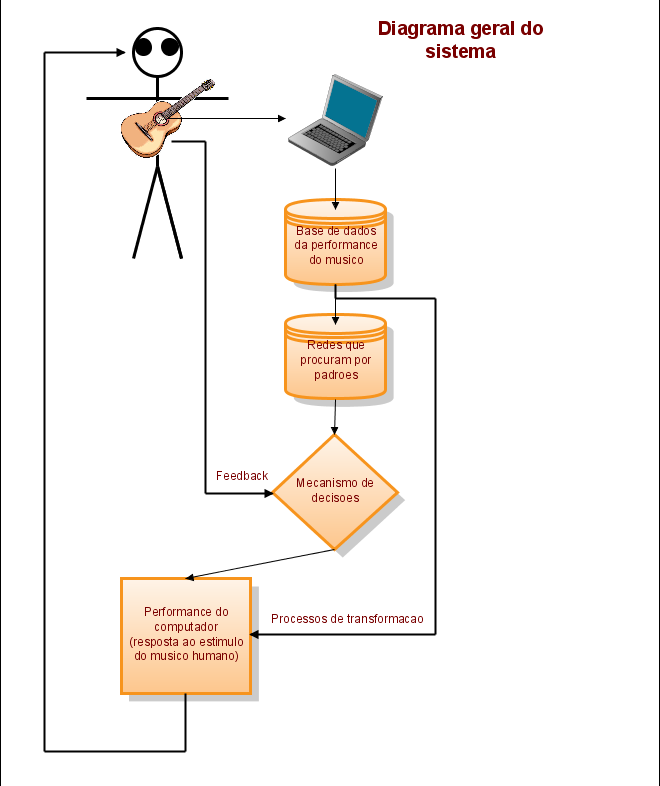
\includegraphics[scale=.7]{geral}
\caption{Diagrama geral do sistema}
\label{geral}
\end{figure}

A figura \ref{escuta} representa o planejamento inicial do projeto onde podemos observar como a 
análise do áudio vai ser separada nos parâmetros de
densidade, durações, classes de intervalos, variações de timbre e registro. Cada parâmetro vai 
passar por uma cadeia de redes locais de tamanhos diferentes que vão ser agrupadas em duas 
redes globais também de tamanhos diferentes.

%colocar parágrafo de como que está agora

%Na figura\ref{mecanismo}

\begin{figure}[!h]
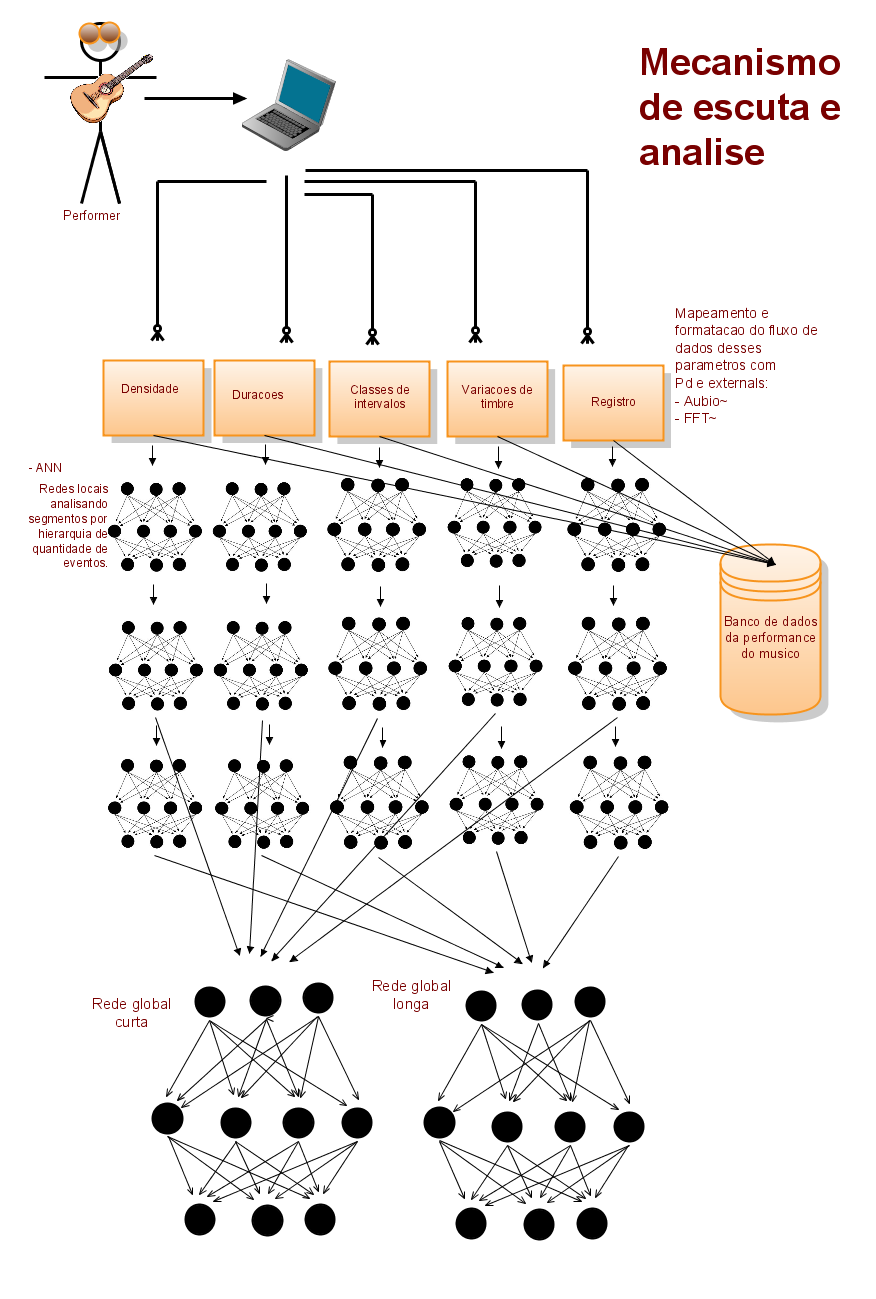
\includegraphics[scale=.7]{escuta}
\caption{Mecanismo de escuta e análise}
\label{escuta}
\end{figure}


A terceira fase será a fase de redação da tese onde serão abordados
todas as especificações técnicas de como o sistema foi construído além
de uma discussão teórica sobre os limites da interação homem-máquina e
o estado da arte dos sistemas musicais interativos. Ao longo das três
fases da pesquisa serão compostas diversas peças que explorem partes
do sistema. A partir da experiência passada durante o mestrado é
esperado que essas composições revelem aspectos fortes e fracos do
sistema e sejam uma bússola que controle o fluxo do desenvolvimento do
sistema.

\section{Glossário}
\label{glossario}


\textbf{Pitch}: Termo relativo a altura das notas, em alguns módulos da pesquisa,
o valor de pitch aparece como um símbolo da nota seguido da oitava respectiva (D4, se
referindo a nota ré da oitava central do piano). Em outros momentos o valor de pitch
se refere ao parâmetro MIDI de 0 a 127. Algumas funções convertem valores puros de frequência
em pitch.

%% acrescentar que frequência é medida numa distribuição exponencial e pitch está disposto
% numa distribuição linear.

\textbf{MIDI}: É a sigla para \textit{Musical Instrument Digital Interface} e descreve um protocolo padrão da indústria, 
definido pela primeira vez em 1982, que permite que instrumentos musicais eletrônicos 
(sintetizadores e máquinas geradoras de som), computadores e outros equipamentos eletrônicos (controladores MIDI , 
placas de som, samplers) se comuniquem e se sincronizem um com o outro. 
As principais funções MIDI incluem comunicação de mensagens de eventos sobre a notação musical,  variação de altura, 
intensidade, sinais de controle para os parâmetros (tais como volume, vibrato, panning, pistas e sinais de 
clock (para definir o tempo)) entre dois dispositivos, a fim de completar uma cadeia de sinal e produzir som 
audível a partir de uma fonte de som. Como um protocolo eletrônico, é notável pela sua adoção generalizada em 
toda a indústria da música.


\textbf{Envelope}: É a definição de como a amplitude de cada nota se comporta.
É um termo comum nas especificações de síntese sonora e é um aspecto decisivo na construção e 
definição do timbre. Normalmente se dividem as fases do
envelope sonoro em ataque, decaimento, sustentação e finalização (ADSR). Por
exemplo, o timbre de um tambor tem um ataque curto, nenhuma sustentação
e uma rápida finalização.

\textbf{Pure data (Pd)}: É uma linguagem de programação visual desenvolvida por Miller Puckette na década de 1990 
para criar música computacional interativa e obras multimídia. Enquanto que Puckette é o autor principal do programa, 
o Pd é um projeto open source que conta com uma base de desenvolvedores trabalhando em novas extensões e funcionalidades.
Ele é liberado sob uma licença similar à licença BSD. Ele roda em GNU/Linux, Mac OSX, iOS, Android e Windows. 
Versões mais antigas ainda existem para FreeBSD e IRIX.

\textbf{Objetos}: ou abstrações em Pd são notadas ao longo do texto entre colchetes,
por exemplo: [abs-musical-pitch-tempo-amp] significa que esse objeto pertence a biblioteca de utilitários
e retorna uma lista com a nota, o tempo e a amplitude de cada nota num sinal de áudio monofônico.

São funções pré-compiladas que providem uma variedade de funções.



\textbf{Patchs}:

\textbf{Sub-patchs}: É um objeto que guarda uma porção de código encapsulado, funciona
de forma local, ou seja, restrito ao patch principal.

\textbf{Abstrações}: Também é um objeto que guarda uma porção de código encapsulado,
porém pode agir de maneira global, uma vez que é salvo separadamente.

\textbf{int, float}:

\textbf{Biblioteca} é um conjunto de objetos para determinada função.O desenvolvimento
central do Pd é nos objetos de matemática e processamento de sinal de áudio. Enquanto
que a comunidade implementou diversas bibliotecas para processamento de vídeo e sensores
de controle. Ao longo do texto iremos usar uma notação do tipo: [objeto\_teste] para
representar um objeto.

\textbf{Mensagens}: São sequências de valores, listas ou métodos de funcionamento para os objetos,
e são grafados da maneira [mensagem lista 1 2 3(.

\textbf{Caixas de número}: normalmente são usadas para teste, manipulação e/ou vizualisação
dos dados em tempo real.

\textbf{Símbolos}: Símbolo do tipo String.

\textbf{Comentários}: Ferramenta de documentação local dos patchs.

\textbf{Objetos gráficos}: Alguns são úteis como sliders e botões diversos.

\textbf{Arrays}: Tabelas de uma dimensão que podem ser utilizados por qualquer objeto
que interprete formatos diversos, desde arquivos de áudio .wav até arquivos de 
texto puro.



\begin{figure}[!h]
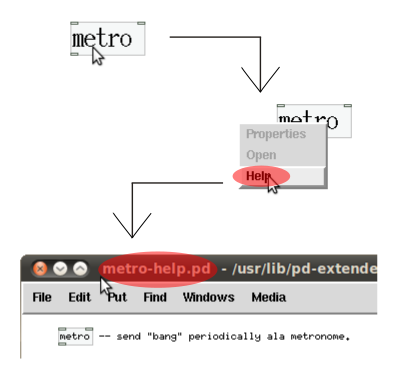
\includegraphics[scale=.6]{help}
\caption{exemplo de acesso ao manual do objeto metro}
\label{help}
\end{figure}


\textbf{Manual do objeto}: Se trata de um patch que exemplifica o uso de determinado
objeto. O próprio editor gráfico do Pd entende que um patch que tenha o nome do objeto 
acrescido de "-help" é referenciado no menu disponível com o clique direito do mouse. 
Na figura \ref{help} vemos que o objeto metro tem o manual
referenciando o patch metro-help.pd acessando um 
menu com o botão direito em cima do objeto em questão.




\textbf{Sampler}:


\textbf{Mixer}

\textbf{Loop}


\section{Idiomas específicos}

Nessa seção devo falar de idiomas específicos de programação com pd como:


\begin{itemize}
 
 \item escrita em arrays
 \item conexão por cabos vs [send] [receive]
 \item variáveis locais vs variáveis globais
 \item objetos gráficos GUI's, subpatchs/abstrações e canvas
 \item objeto [expr] vs. sequência de objetos
 \item Diferenças entre mensagens de controle e fluxo de áudio
 \item amplificação de áudio

\end{itemize}



\section{Ferramentas}

Nessa seção devo falar de:

\subsection{GNU/linux}

* filosofia GNU vs flexibilidade linux

* ciência e arte como atitudes políticas

* porque da eficácia do linux

* distros - ubuntu





\subsection{git}


screenshots

\subsection{jack}


alsa 

screenshots


\subsection{rosegarden}

MIDI

soundfont

lilypond

 

\subsection{Pd-extended}


- pdextended vs. pd vanilla e compatibilidades
- versões

\subsection{Bibliotecas de Pd}

- pdmtl e DIY
- objetos "tabletools" e "timbreId" 


%\begin{figure}
%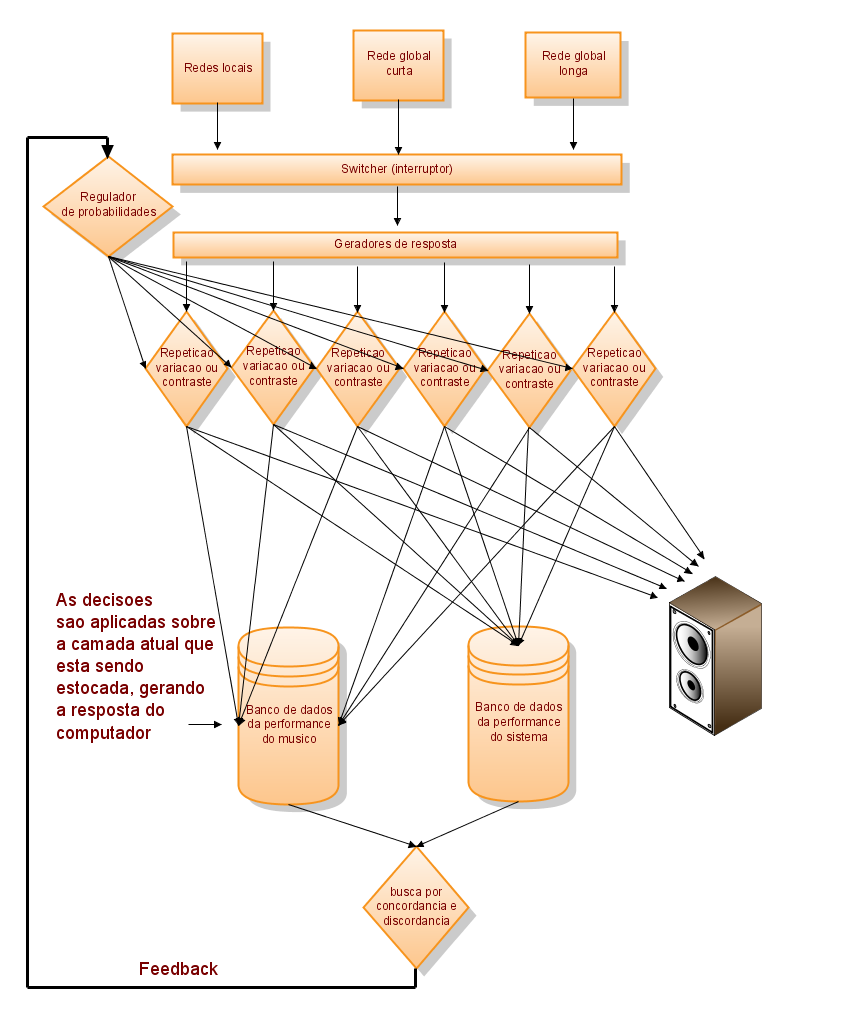
\includegraphics[scale=.6]{mecanismo}
%\caption{Mecanismo de decisões e geração de resposta}
%\label{mecanismo}
%\end{figure}



\newpage


\section{restrições/limitações}


Discussão da problemática de análise de áudio
em tempo real de instrumentos polifônicos.

Apresentar a solução do Miller (patch for guitar).


\chapter{SInCoPA}
\label{chap:SInCoPA}


  Nesse capítulo serão expostas as abstrações desenvolvidas para o sistema, como também
os protótipos e programas auxiliares desenvolvidos para explicar o uso correto das 
abstrações apresentadas. O conjunto de abstrações cumprem funções básicas necessárias
a projetos de música interativa que relacionem análise de áudio e geradores musicais
baseados nos dados da análise do áudio de entrada em tempo-real.


  Foi desenvolvida uma biblioteca de funções utilitárias em forma de abstrações, 
tornando fácil seu re-uso em outros projetos. As abstrações se dividem em 7 categorias:

\begin{enumerate}
 \item Análise de áudio de entrada em tempo-real;
 \item Geradores MIDI baseados no comportamento do áudio de 
entrada, com variações de controle, indo da mímese do sinal de entrada
até um grau mais elevado de contraste rítmico e melódico;
 \item Geradores de síntese sonora, também baseados no comportamento
do áudio de entrada com diversos níveis de controle;
 \item Módulos de processamento de sinal, usados no áudio de entrada e no
áudio gerado pela comunicação MIDI;
 \item Vizualizador de notação musical do áudio de entrada e de saída;
 \item Cenários de comportamentos interativos e Mixer de volumes responsivo;
 
\end{enumerate}


Uma composição musical usando o SInCoPA, consiste na concatenação de
regras que coordenam os comportamentos das várias partes envolvidas.
Esse conjunto de regras foi denominado de ``cenário''. Na composição
de um cenário o compositor escolhe, por exemplo,  se determinado gerador 
deve ter um comportamento complementar ou contrastante  em relação a algum
parâmetro de análise.



%% testar esse novo teclado - falar sobre o controlador pedal 

%% aqui pra cada patch um formato de projeto:
%% intro + objetivo + justificativa + metodologia+ conclusão e desenvolvimento futuro


%%\subsection{Biblioteca de Utilitários}

\section{Análise de áudio}

Nessa seção serão apresentados os problemas e soluções específicos
a análise de áudio. 

É importante a flexibilização para a detecção de parâmetros musicais.
Também é importante a possibilidade de salvar os dados das análises serem
destacados nas interfaces dos objetos.

A interface gráfica dos objetos prevê vizualização em tempo-real
da atividade no módulo de análise e botões descritos para controle
de parâmetros diversos.


\subsection{Entrada de áudio}

Um elemento importante na interface é a vizualização instantânea
do fluxo de áudio. Aqui na figura \ref{audioin} apresentamos uma solução prática e podemos
ver uma outra abordagem nas figuras \ref{fft_geral} e \ref{fft_aaray} baseada em análise FFT.

\subsubsection{Objeto [sinc-audioin]}


\begin{figure}[!h]
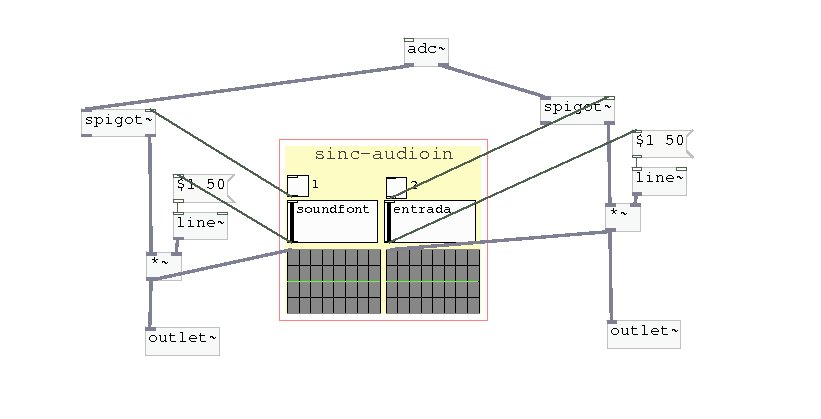
\includegraphics[scale=.55]{audioin}
\caption{Entrada de áudio [sinc-audioin]}
\label{audioin}
\end{figure}

A entrada de áudio no pd começa com o objeto  [adc\texttildelow], e sempre segue um fluxo
básico que passa por um objeto de multiplicação de sinal [*\texttildelow] que permite um
controle manual de entrada de áudio. Esse controle é necessário para ajustar 
a sensibilidade dos objetos que realizarão a análise de áudio. A abstração 
[sinc-audioin] na figura \ref{audioin} permite o roteamento e vizualização rápida 
de entrada de áudio de dois canais. No caso dos experimentos musicais envolvidos 
nessa pesquisa, foi estabelecido o canal 1 para o recebimento de áudio do programa 
rosegarden, que hospeda samplers do tipo ``soundfont''. O canal 2 é usado para 
a entrada de áudio do instrumento. É necessário um objeto que funcione como uma chave de
liga/desliga para o áudio. Para isso foi usado o objeto [spigot\texttildelow] da biblioteca
``Unauthorized'' incluída no pd-extended.
 Quando o toggle([tgl]) é acionado com clique de mouse,
ele envia o valor 1 pela saída que por sua vez está conectado na entrada fria do
[spigot\texttildelow], essa ação faz com que o áudio seja liberado pela saída do [spigot\texttildelow].
Os volumes de entrada são controlados por objetos gráficos sliders ([hsl]), que tem
a saída ligada a uma variável de parâmetro para o objeto [line\texttildelow]. Nesse caso específico
[line\texttildelow] atua no sentido de se evitar cliques no áudio quando se muda o valor de 
amplitude que entra na entrada fria do objeto [*\texttildelow]. Outro componente
opcional, que é útil em situações práticas, é um vizualizador gráfico de presença de sinal
de áudio. Em [sinc-audioin] é usado o objeto [Scope\texttildelow] da biblioteca ``cyclone'', 
incluída no pd-extended.

%% dar uma olhada no livro do Miller sobre [*~] e [line~] 

\subsection{Manipulação de amostras}


  Dentro do  contexto de laboratório de prototipação, se faz necessário emular uma entrada 
de áudio em tempo-real com a execução de trechos de áudio sampleados ou um sintetizador simples
com entrada de notas pelo teclado alfa-numérico do computador. Nesse sentido foram construídas
algumas abstrações para facilitar o processo de desenvolvimento e teste.

\subsubsection{Objeto [sinc-sample]}



\begin{figure}[!h]
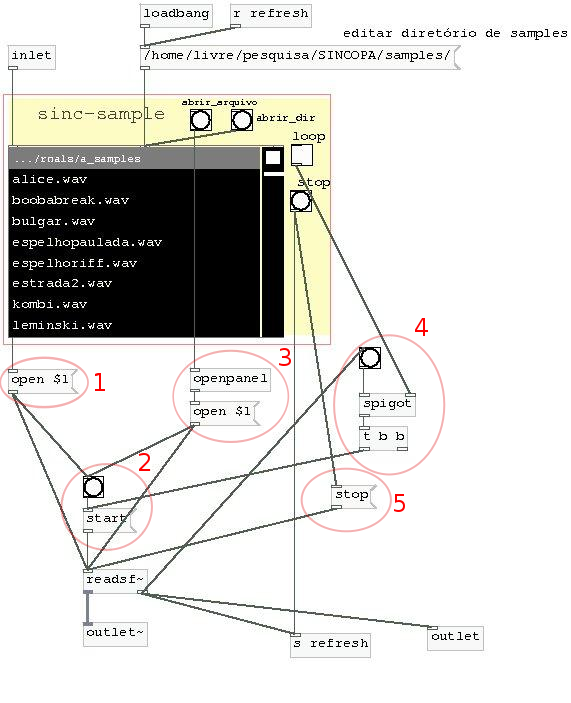
\includegraphics[scale=.5]{sinc-sample}
\caption{[sinc-sample]}
\label{[sinc-sample]}
\end{figure}



A primeira a ser desenvolvida foi a abstração [sinc-sample] mostrado na figura
\ref{[sinc-sample]}. Para essa abstração foi escolhida a abstração gráfica 
[file.browser] 
na área 1 circulada na figura \ref{[sinc-sample]} que lê os arquivos de determinado
 diretório e lista eles graficamente possibilitando que
o usuário clique no nome do arquivo escolhido, resultando em uma mensagem com a 
localização
do arquivo. Essa abstração faz parte do pacote ``pdmtl'' de abstrações de pd.
A execução do áudio é feita com o objeto [readsf\texttildelow] que precisa de três mensagens:
start, stop e localização do arquivo. O mecanismo grifado na área 2, mostra
um objeto [trigger]([t]) realizando uma tarefa em 3 fases da direita para a esquerda:
\begin{itemize}
 \item Aciona a mensagem com o caminho do arquivo a ser tocado
 \item Aciona a mensagem ``start''
 \item Recarrega a mensagem que atualiza o diretório a ser lido por [file.browser]
\end{itemize}

Outro aspecto dessa abstração é a possibilidade de tocar um arquivo de áudio em loop.
Na área circulada 4 temos um [spigot] que atua como interruptor de um bang enviado pela
saída direita de [readsf\texttildelow], que por sua vez é enviado quando [readsf\texttildelow] 
acaba de ler o arquivo
inteiro. Se o toggle que está conectado com o [spigot] da área 4 estiver ligado, ele permite
que o bang enviado ao final da leitura seja roteado para outro objeto trigger que aciona as 
duas primeiras fases descritas acima, realizando uma leitura contínua do arquivo de áudio
escolhido.



\subsection{Análise melódica}


Existem diversos problemas de pesquisa relacionados com a
análise melódica como por exemplo:

\begin{itemize}
 \item Detecção de notas;
 \item Estimativa de nota;
 \item Conversão de fluxo de áudio em dados semânticos (MIDI);
 \item Permeabilidade melódica;
 \item Análise de contorno e direcionamento melódico;
\end{itemize}




\subsubsection{Objeto [sinc-audioanalise]}

Um dos fatores mais importantes para a prática de análise melódica
em tempo real é a flexibilidade de refinamento dos parâmetros
de análise. Esses parâmetros devem estar ao alcance rápido e documentados
e sinalizados na interface.


Nessa abstração procurou-se desenvolver uma interface que facilite
a rápida prototipação e flexibilidade de parâmetros que podem
se adaptar facilmente para diferentes fontes sonoras.

\begin{figure}[!h]
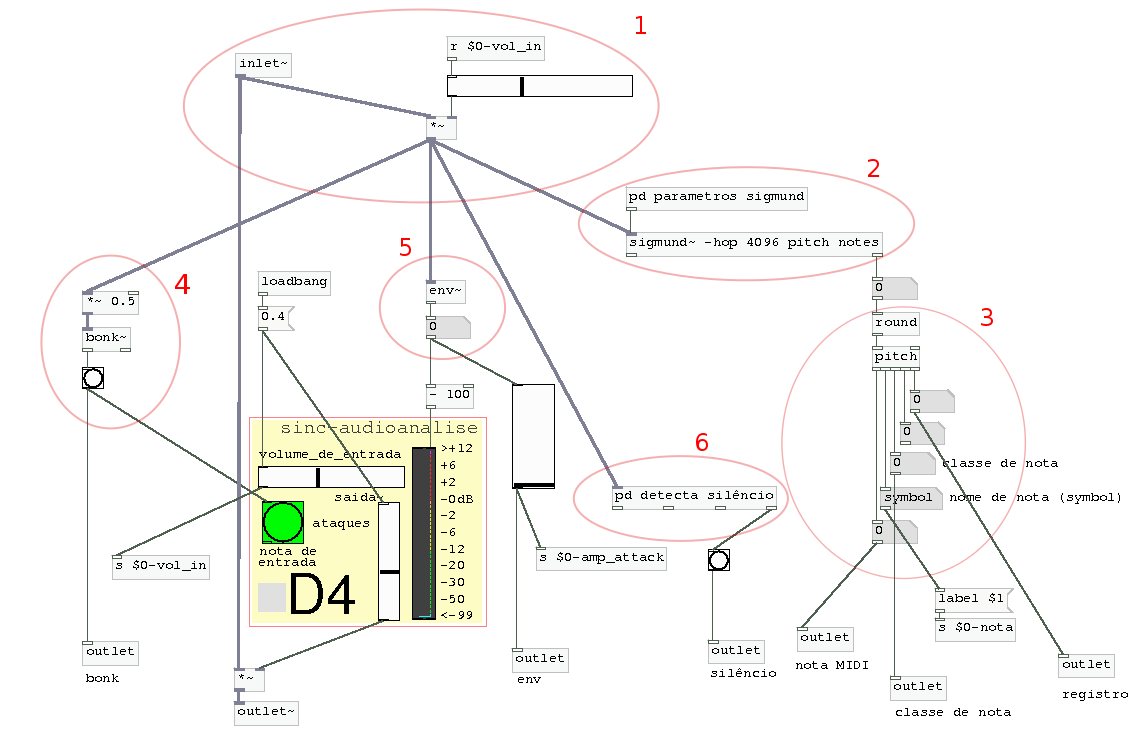
\includegraphics[scale=.4]{sinc-audioanalise}
\caption{[sinc-audioanalise]}
\label{[sinc-audioanalise]}
\end{figure}

Como podemos ver na área 1 da figura \ref{[sinc-audioanalise]},
temos o controle de um slider vertical\footnote{objeto [hslider]}
controlando a amplitude geral do áudio de entrada. Esse controle
é muito importante em situações em que se tem variações de amplificação
entre ensaios e performance.

%%Área 1: explicação da amplificação de volume de entrada/volume de saída

\begin{figure}[!h]
\includegraphics[scale=.5]{sinc-audioanalise_param}
\caption{sub-patch que controla as configurações de [sigmund\texttildelow]}
\label{[sinc-audioanalise_param]}
\end{figure}


Na área 2 aparece um subpatch que pode ser visto na figura
\ref{[sinc-audioanalise_param]}. Nesse subpatch podemos ver 
a organização dos parâmetros do objeto [sigmund\texttildelow].

O objeto [sigmund\texttildelow] faz análise de áudio no domínio da 
frequência e detecção de notas. Os parâmetros podem ser re-definidos
em tempo-real através dos argumentos de criação do objeto ou através
de mensagens como é o caso aqui.


Segundo a documentação no próprio manual do objeto:

\begin{quote}
 Sigmund\texttildelow analyzes an incoming sound into sinusoidal
components, which may be reported individually or combined to
form a pitch estimate. Possible outputs are specified as creation
arguments:

\begin{itemize}
 \item pitch - output continuously
 \item notes - output pitch at the beginning of notes
 \item env - output amplitude continuously
 \item peaks - output all sinusoidal peaks in order of amplitude
 \item tracks - output sinusoidal peaks organized into tracks
\end{itemize}
Parameters you may set (in cretaion arguments or messages):

\begin{itemize}
 \item npts - number of points in each analysis window (1024)
 \item hop - number of points between each analysis (512)
 \item npeak - number of sinusoidal peaks (20)
 \item maxfreak - maximum sinusoid frequency in Hz. (1000000)
 \item vibrato - depth of vibrato to expect in 1/2 tones (1)
 \item stabletime - time (msec) to wait to report notes (50)
 \item minpower - minimum power (dB) to report a pitch (50)
 \item growth - growth (dB) to repor a new note (7) 
\end{itemize}
The npts and hop parameters are in samples. and are powers of two.
\end{quote} 


\begin{figure}[!h]
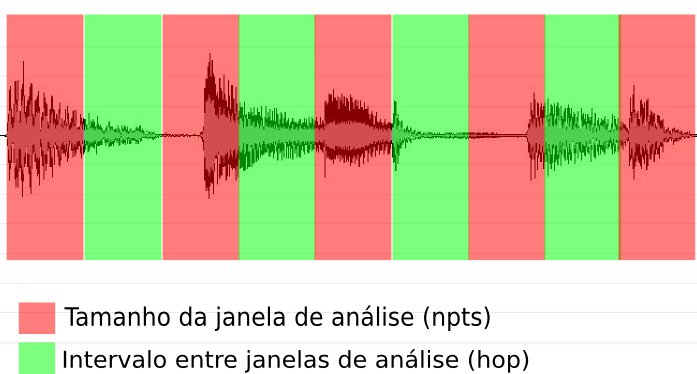
\includegraphics[scale=.7]{sigmund}
\caption{Tamanho de janela de análise (npts)}
\label{janela_analise}
\end{figure}


Nesse caso optou-se por pré-inicializar [sigmund\texttildelow] com as
opções : "-hop 4096 pitch notes" . Através de testes empíricos preferiu-se
usar apenas a saída de "notes" por apresentar uma saída mais precisa para notas 
musicais. A mensagem em destaque na figura \ref{[sinc-audioanalise_param]} representa
a inicialização dos valores de todos parâmetros de [sigmund\texttildelow].

Os principais parâmetros definem o tamanho da janela de análise.
Nesse caso "npts" e "hop" tem uma relação direta
por se tratar do tamanho da janela de análise e o espaço
entre as janelas em samples como pode ser visto na figura \ref{janela_analise}.



%%Área 2: explicação do sigmund~ - ver livro Miller + help do sigmund~


\begin{figure}[!h]
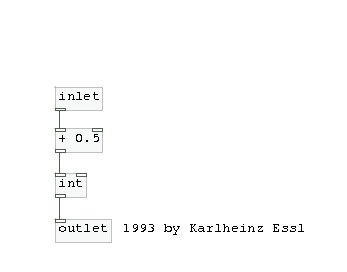
\includegraphics[scale=.5]{round}
\caption{[round]}
\label{round}
\end{figure}


Na área 3 vemos o objeto [round], presente na biblioteca RTC, responsável
por arredondar o valor de entrada para cima. O arredondamento é feito com
a soma de 0.5 e transformação do número do tipo float para tipo inteiro ([int]),
como pode ser visto na figura \ref{round}.


\begin{figure}[!h]
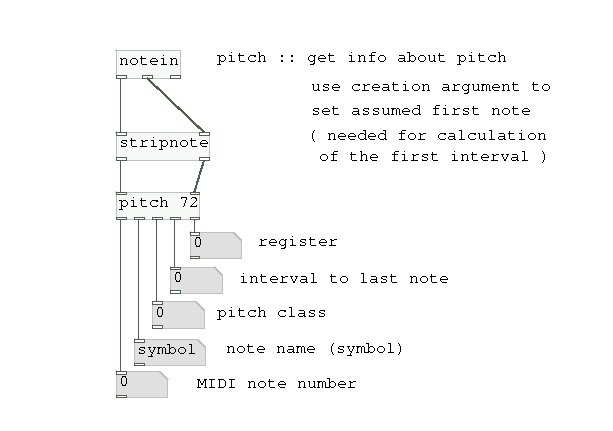
\includegraphics[scale=.5]{pitch}
\caption{[pitch]}
\label{pitch}
\end{figure}


\begin{figure}[!h]
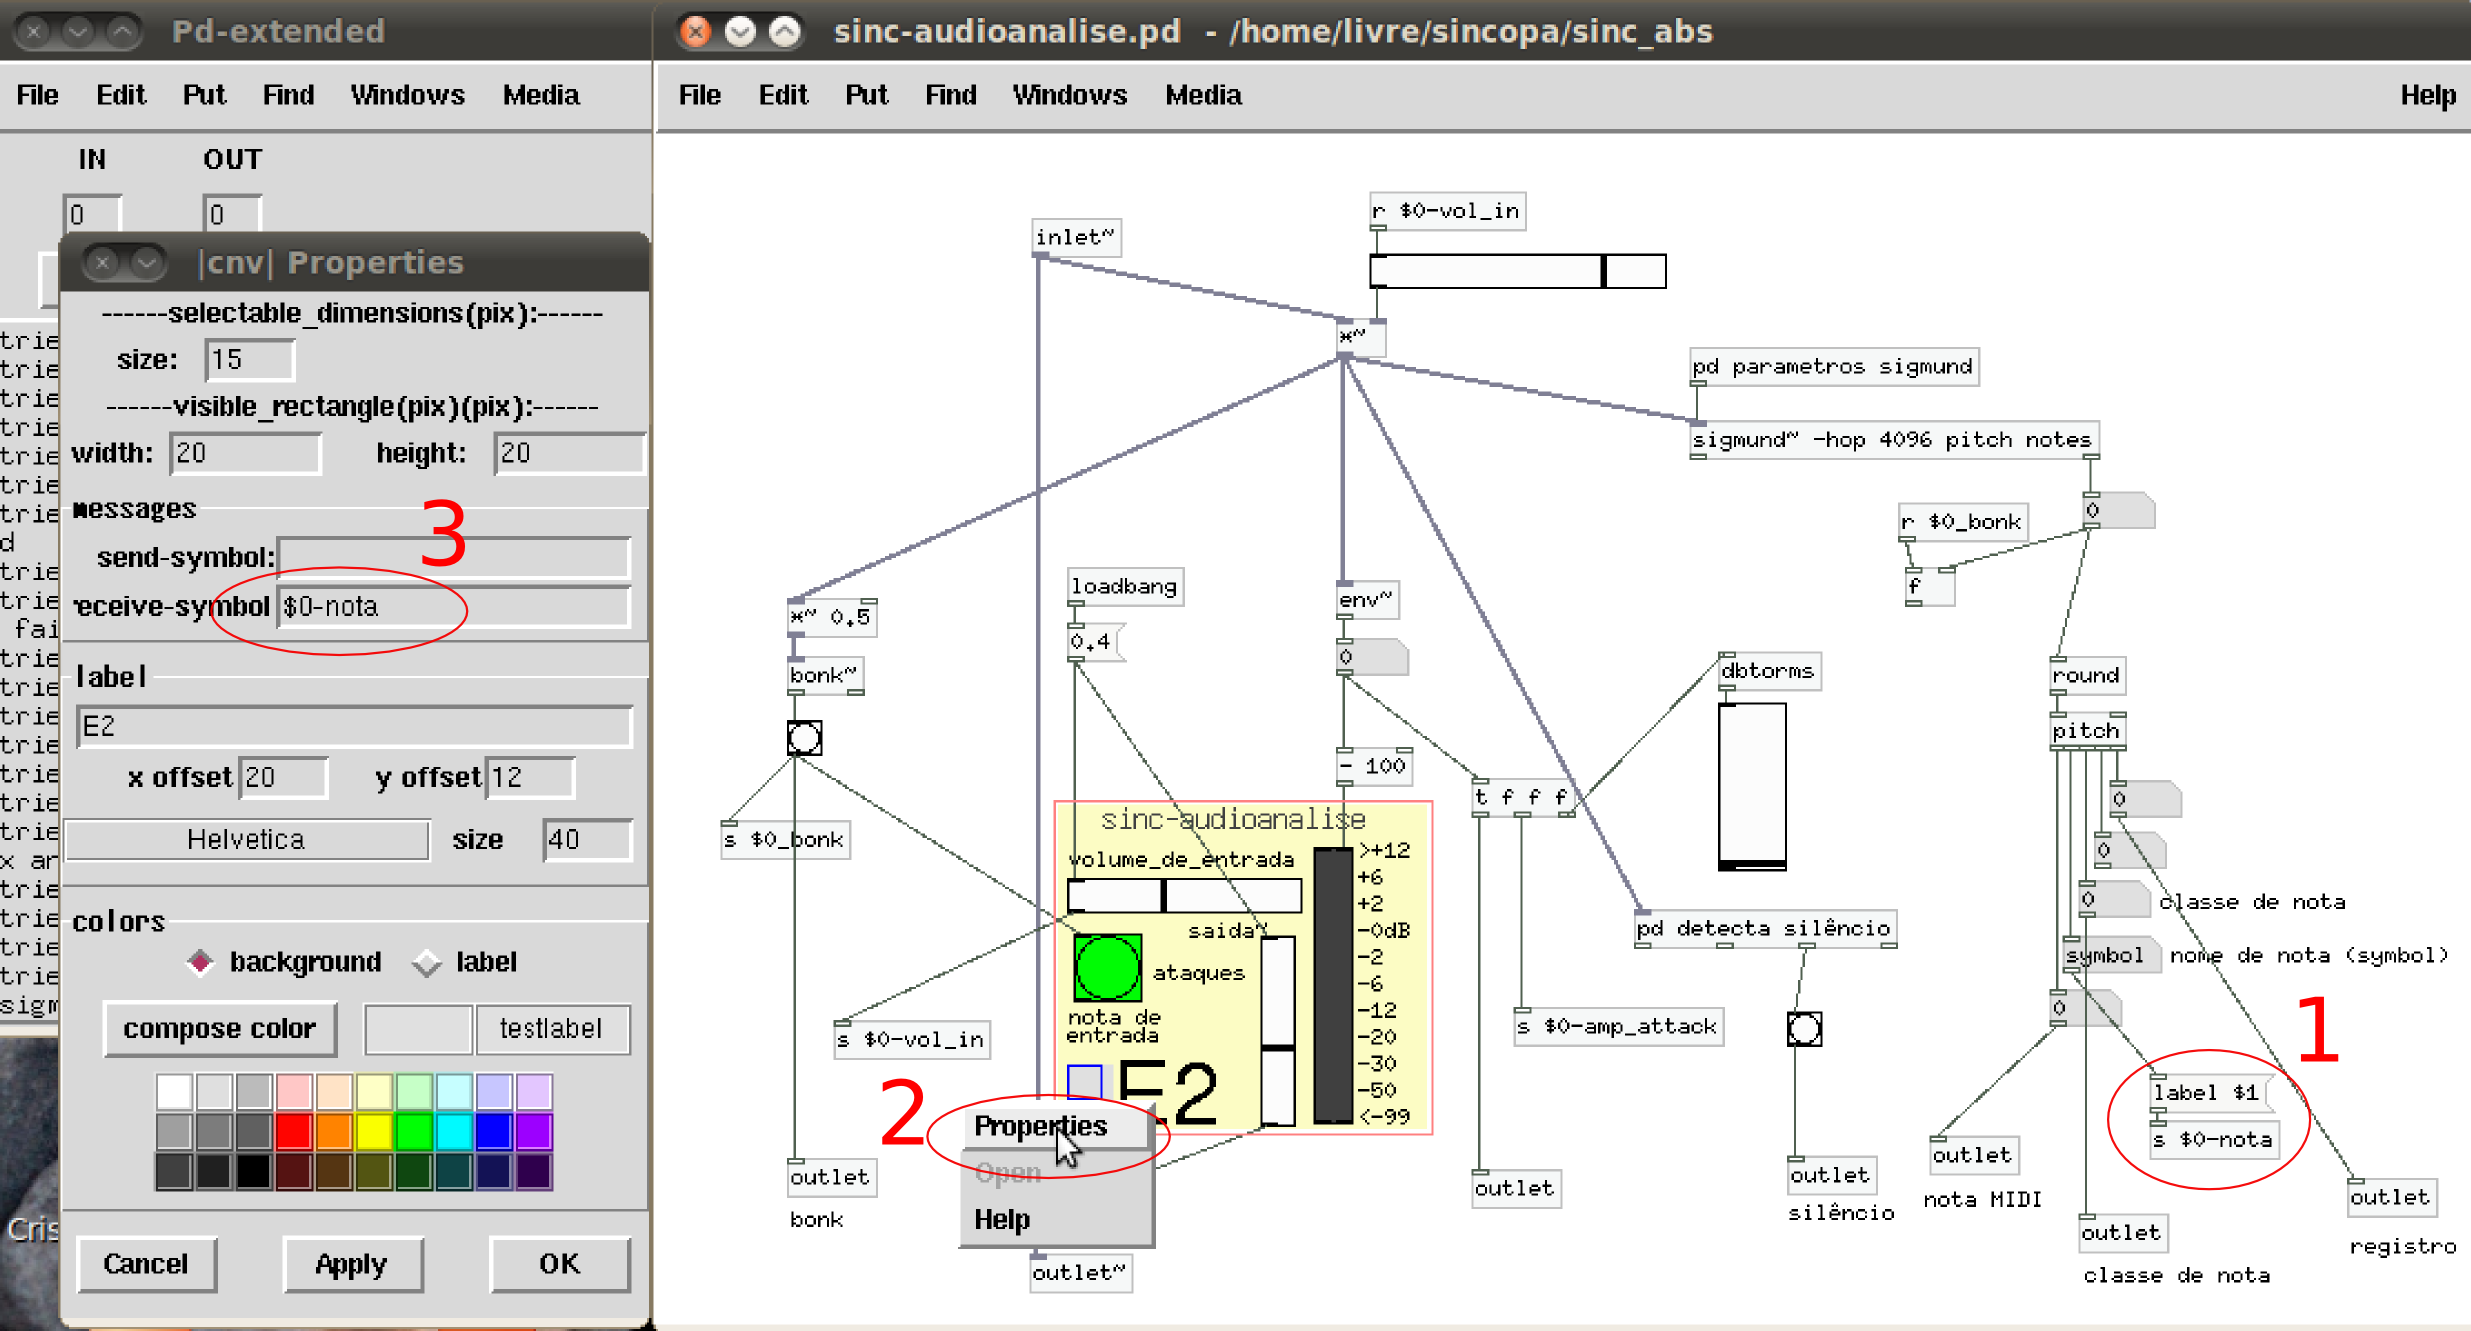
\includegraphics[scale=.5]{canvas-edit}
\caption{editando objeto canvas ([cnv])}
\label{canvas-edit}
\end{figure}


O objeto [pitch] pertence a biblioteca maxlib, distribuída junto com o 
pd-extended e sua funcionalidade pode ser vista no próprio help do objeto na 
figura \ref{pitch}. A interface gráfica de [sinc-audioanalise] mostra o pitch
da nota detectada em tempo-real. A vizualização é feita com o objeto canvas ([cnv]).
A segunda saída do objeto [pitch] retorna um símbolo com a cifra e oitava
da nota. Esse símbolo é enviado para o canvas com o método "label" através
da variável \$0-nota. O objeto canvas aceita variáveis enviadas com o objeto [send],
editando as propriedades do canvas (ver figura \ref{canvas-edit}). A vizualização em tempo-real
é indispensável para calibrar a análise de áudio.


%%Área 3: explicação de round e pitch + plotar cifra no canvas


Na área 4 vemos o objeto [bonk\texttildelow] 



%%Área 4: explicação do bonk~

Na área 5 vemos o objeto [env\texttildelow]. Esse objeto recebe um sinal de áudio
e retorna a amplitude RMS em decibéis (com o valor 1 normalizado para 100 dB).
A saída tem o limite inferior em zero. O algoritmo de análise interna de [env\texttildelow]
usa uma janela de análise do tipo "Hanning" (raised cosine). Uma boa aplicação de 
[env\texttildelow] é mandando o resultado da saída para o objeto [dbtorms] que transforma
os valores em decibéis em uma escala linear, que é uma distribuição melhor para vizualização
gráfica da variação de amplitude.






\begin{figure}[!h]
\includegraphics[scale=.5]{sinc-audioanalise_detecta}
\caption{sub-patch que detecta silêncio no áudio de entrada}
\label{[sinc-audioanalise_detecta]}
\end{figure}




Na área 6 vemos um subpatch responsável por detectar
silêncio. Na figura \ref{[sinc-audioanalise_detecta]}


Nesse sub-patch vemos 4 sub-áreas. Nessa implementação
está sendo usada apenas a terceira saída que é a saída do
módulo de detecção de silêncio. O módulo da sub-área 3
basicamente compara as amplitudes que recebe com relação ao tempo.
Nesse algoritmo, se a amplitude de entrada for menor que 45 dB durante
mais de 100 milisegundos um silêncio é detectado.



\subsection{Análise rítmica}

Se considerarmos que um evento sonoro pode ser descrito por um espaço multidimensional
onde cada parâmetro seria uma dimensão (notas, registros, timbre, etc..), podemos
imaginar o ritmo como uma outra multidimensão paralela e sincronizada com as outras.
O aspecto rítmico de um evento sonoro pode ser descrito por:
\begin{itemize}
 \item relações de durações entre ataques de notas;
\item relações de acento (amplitude) entre ataques de notas;
\item densidade de eventos em recortes de tempo;
\item descrição de índices de estabilidade em diferentes recortes temporais;
\end{itemize}

Todos esses níveis se entrecruzam para formar um cenário que pode explicar mais detalhadamente
os elementos rítmicos de um evento sonoro. O objetivo dessa seção é apresentar o desenvolvimento de
ferramentas para a análise das múltiplas camadas de descrição do ritmo.


Aqui apresentar exemplos com formas de onda em arrays e mostrando na figura
onde é mais denso, onde é mais instável e hierarquia de intensidade em trechos.

Mostrar também trechos maiores com índices de estabilidade.



\subsubsection{Objeto [sinc-calc\_ritmo]}

Uma das questões perseguidas é o fato do sistema ter conhecimento do atual nível de 
estabilidade rítmica. Isso pode ser alcançado por uma relação que considere variações
de pulso e alternância e variações de padrões rítmicos de tamanhos diferentes.

\begin{figure}[!h]
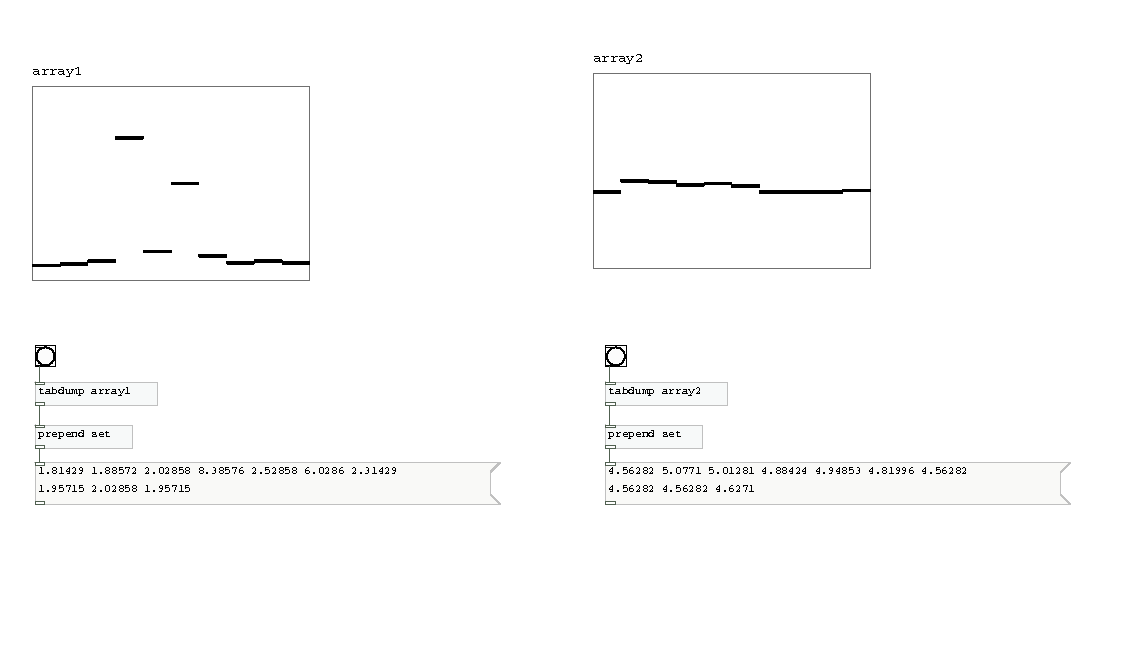
\includegraphics[scale=.6]{prot5a}
\caption{análise de estabilidade rítmica}
\label{prot5a}
\end{figure} 

Na \ref{prot5a} é mostrado dois arrays, idealmente esses arrays representam tabelas
de probabilidades de padrões rítmicos, onde cada elemento no array representa um
padrão diferente e quanto mais alto significa que teve mais ocorrẽncias.
Por exemplo, cada vez que um determinado padrão de 4 valores de duração é tocado, 
o índice na tabela correspondente a aquele padrão é incrementado. O objetivo ideal
é um mecanismo que possa retornar uma resposta do tipo:
``o array1 é mais estável que o array2''. Apenas olhando fica fácil de identificarmos
no array1 que os padrões 3 e 5 tem mais probabilidade de ocorrer pelo seu histórico,
contribuindo assim para uma sensação de estabilidade rítmica. Enquanto que o array2,
tem probabilidades próximas de quase todos padrões criando uma sensação de imprevisibilidade
e fragmentação.

\begin{figure}[!h]
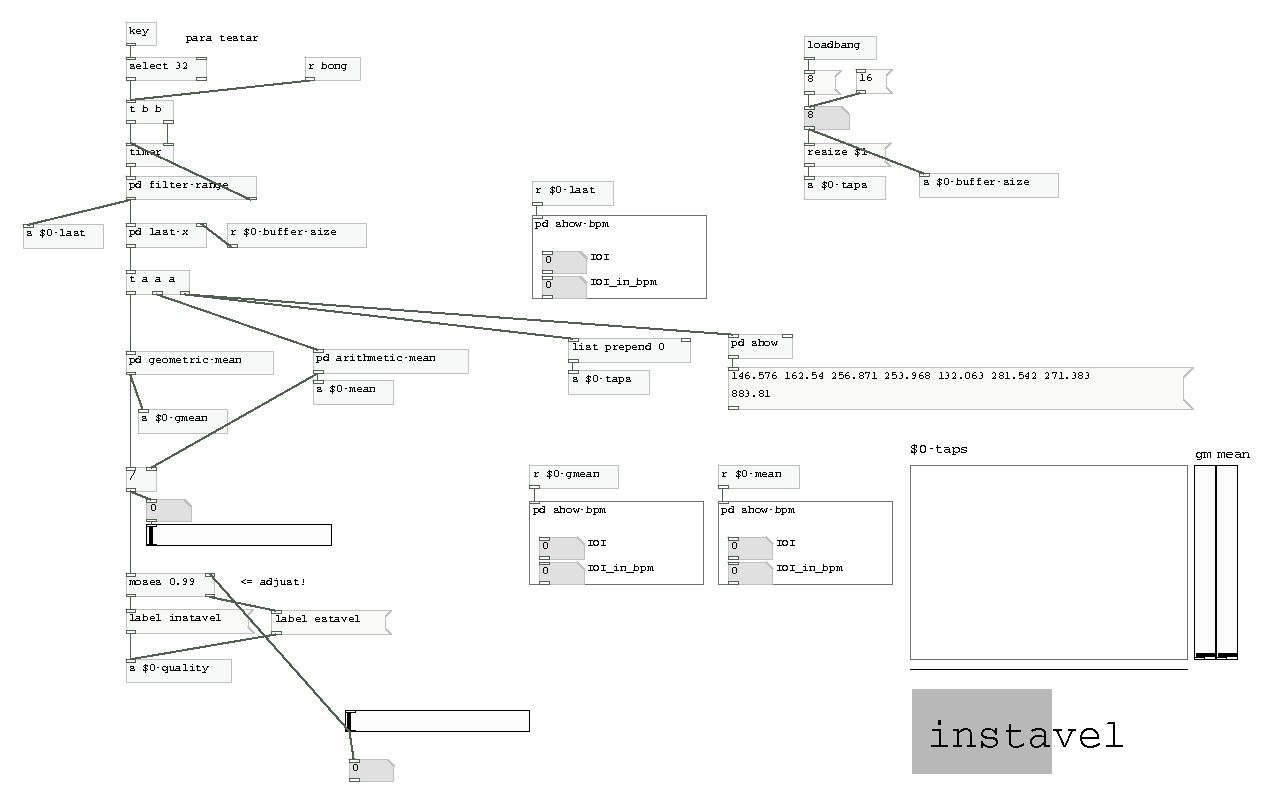
\includegraphics[scale=.55]{prot5d}
\caption{Índice de estabilidade de pulso}
\label{prot5d}
\end{figure}


No patch da \ref{prot5d} é apresentado um método de classificação de estabilidade
de sequência de pulsos. Primeiro são calculadas as distâncias entre cada ataque
sonoro, depois filtrado em [pd filter-range] e colocado em uma tabela dinâmica em
[pd last-x]. O tamanho da tabela sempre pode ser redimensionado em tempo-real através
da variável \textit{0-buffer-size} então é calculado ao mesmo tempo a média geométrica
e a média aritmética e os resultados são executados na expressão definida por uma
divisão da média geométrica pela média aritmética. %% isso poderia ser definido em notação matemática :)
Ao resultado dessa divisão é aplicado um filtro com [moses] onde se pode calibrar
a sensibilidade do valor do índice final.


\begin{figure}[!h]
\includegraphics[scale=.5]{sinc-calc_ritmo}
\caption{análise de estabilidade rítmica}
\label{[sinc-calc_ritmo]}
\end{figure}

\begin{figure}[!h]
\includegraphics[scale=.5]{sinc-calc_ritmo1}
\caption{filtro de registro de durações}
\label{[sinc-calc_ritmo1]}
\end{figure}

\begin{figure}[!h]
\includegraphics[scale=.5]{sinc-calc_ritmo2}
\caption{lista de durações}
\label{[sinc-calc_ritmo2]}
\end{figure}

\begin{figure}[!h]
\includegraphics[scale=.5]{sinc-calc_ritmo3}
\caption{média geométrica}
\label{[sinc-calc_ritmo3]}
\end{figure}

\begin{figure}[!h]
\includegraphics[scale=.5]{ex_ritmo1}
\caption{ritmo estável}
\label{ex_ritmo1}
\end{figure}

\begin{figure}[!h]
\includegraphics[scale=.5]{ex_ritmo2}
\caption{ritmo instável}
\label{ex_ritmo2}
\end{figure}

\begin{figure}[!h]
\includegraphics[scale=.4]{ex_ritmo3}
\caption{ritmo estável e instável}
\label{ex_ritmo3}
\end{figure}


A técnica básica de análise rítmica em Pd, se dá através do uso do objeto [timer].
O objeto [timer] mede a distância em milisegundos entre "bangs' que chegam pela entrada
da esquerda em relação ao que chega pela entrada da direita.%% aqui mostrar o básico do timer embasado pelo Rowe


Um músico humano sempre realiza micro-variações de tempo e andamento.
Na figura \ref{ex_ritmo1} vemos uma incidência de ataques mantendo uma relação de estabilidade
de durações. Enquanto que na figura \ref{ex_ritmo2} vemos uma relação mais instável
entre as durações. Já na figura \ref{ex_ritmo3} vemos um padrão que se mantém estável e 
muda para um comportamento de instabilidade de durações. Um dos desafios da pesquisa
foi estabelecer uma forma do programa conseguir classificar a estabilidade de cada nova duração em relação
as anteriores.

No patch da figura \ref{[sinc-calc_ritmo]} é apresentado um método de classificação de estabilidade
de durações entre notas. Primeiro são calculadas as distâncias entre cada ataque
sonoro, depois filtrado em [pd filter-range] e colocado em uma tabela dinâmica em
[pd last-x]. O tamanho da tabela sempre pode ser redimensionado em tempo-real através
da variável \textit{0-buffer-size} então é calculado ao mesmo tempo a média geométrica
e a média aritmética e os resultados são executados na expressão definida por uma
divisão da média geométrica pela média aritmética. %% isso poderia ser definido em notação matemática :)


A divisão da média geométrica pela média aritmética pode ser definida pela expressão

\begin{equation}
\frac{n\sqrt[n]{a1.a2....an}}{a1+a2+...an} 
\end{equation}  

Essa expressão é calculada a cada nota que chega, onde n é o tamanho do buffer.
O resultado desse cálculo devolve um valor numa escala de 0 a 1.
Esse valor representa o índice de instabilidade rítmica da última duração entre 2 notas,
comparado com as últimas "n" durações.
Nesse resultado dessa divisão é aplicado um filtro com [moses] onde se pode calibrar
a sensibilidade do valor do índice final.


\subsubsection{Objeto [sinc-densidade]}

%densidade_ritmica.pd em /abs

O que é densidade rítmica e para quê serve.



\begin{figure}[!h]
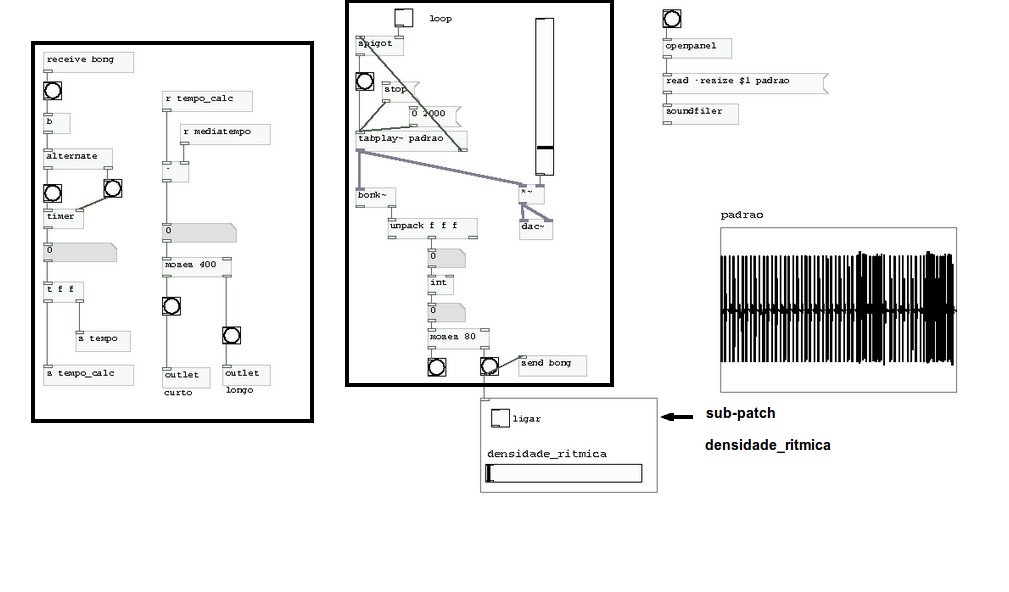
\includegraphics[scale=.5]{prot5b}
\caption{captação de ataques com [bonk\texttildelow] e categorização entre ``curtos'' e ``longos''}
\label{prot5b}
\end{figure}

Os primeiros passos na implementação desse mecanismo podem ser vistos na \ref{prot5b},
onde na área central, aparecem um leitor de samples [tabplay\texttildelow] lendo um arquivo de
áudio e enviando o fluxo de áudio para o objeto [bonk\texttildelow]. A saída de [bonk\texttildelow] é filtrada
pelo objeto [moses] que pode ter um número de corte variável, sendo flexível a diferenças
de volume em diferentes momentos,lugares ou fontes sonoras .

Ainda na \ref{prot5b}, a seção da esquerda mostra uma maneira de classificar as durações
entre ataques de notas em longas ou curtas, possibilitando uma classificação básica,
que vai possibilitar a criação de padrões rítmicos de combinações entre longos e curtos.
Nesse caso também o limite entre longo e curto é dado por [moses] que pode ser redimensionado
em tempo-real. 

\begin{figure}[!h]
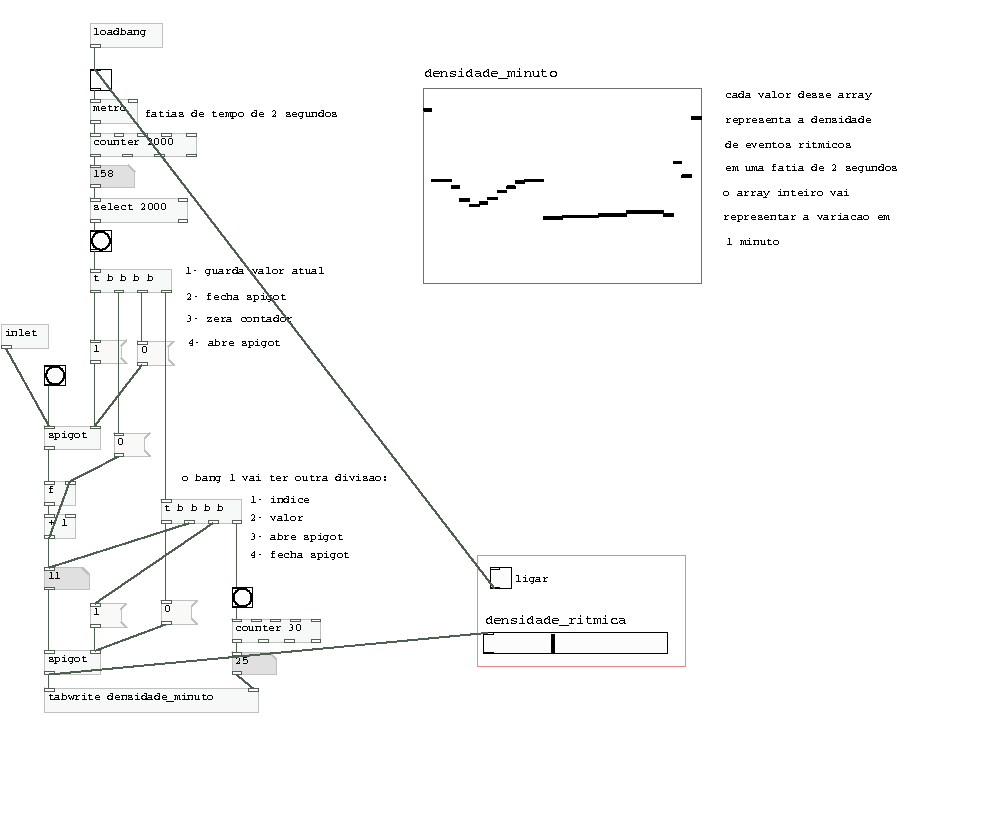
\includegraphics[scale=.75]{prot5c}
\caption{sub-patch [densidade ritmica]}
\label{prot5c}
\end{figure}


Na \ref{prot5c} vemos o conteúdo interno do sub-patch [densidade\_ritmica], onde é realizadas
contagens de quantos ataques de eventos sonoros acontecem a cada 2 segundos de tempo.
Densidade rítmica é um bom índice global de controle dos eventos sonoros por um instrumentista.
A maneira de uso desse índice se transforma de um controle rítmico prático para um
músico treinado.





\subsection{Análise de timbre}

\subsubsection{FFT}

FFT é a sigla para Fast Fourier Transformation, e é a principal técnica para realizar uma análise no domínio 
da frequência. No Pd encontramos o objeto [rfft\texttildelow] que permite o 
acesso aos dados completos da análise do espectro sonoro.
Nessa seção será apresentada uma introdução sucinta a 
análise FFT no Pd e a manipulação dos dados resultantes dessa análise.

Uma explicação mais aprofundada da FFT no Pd é visto no apêndice \label{fftpd}.

* resumo rápido de FFT crua , acessando, visualizando e salvando e recuperando

\subsubsection{[bonk\texttildelow]}

* Bonk~ e tutorial de "learning" do bonk~


\subsubsection{timbreID}

\begin{figure}[!h]
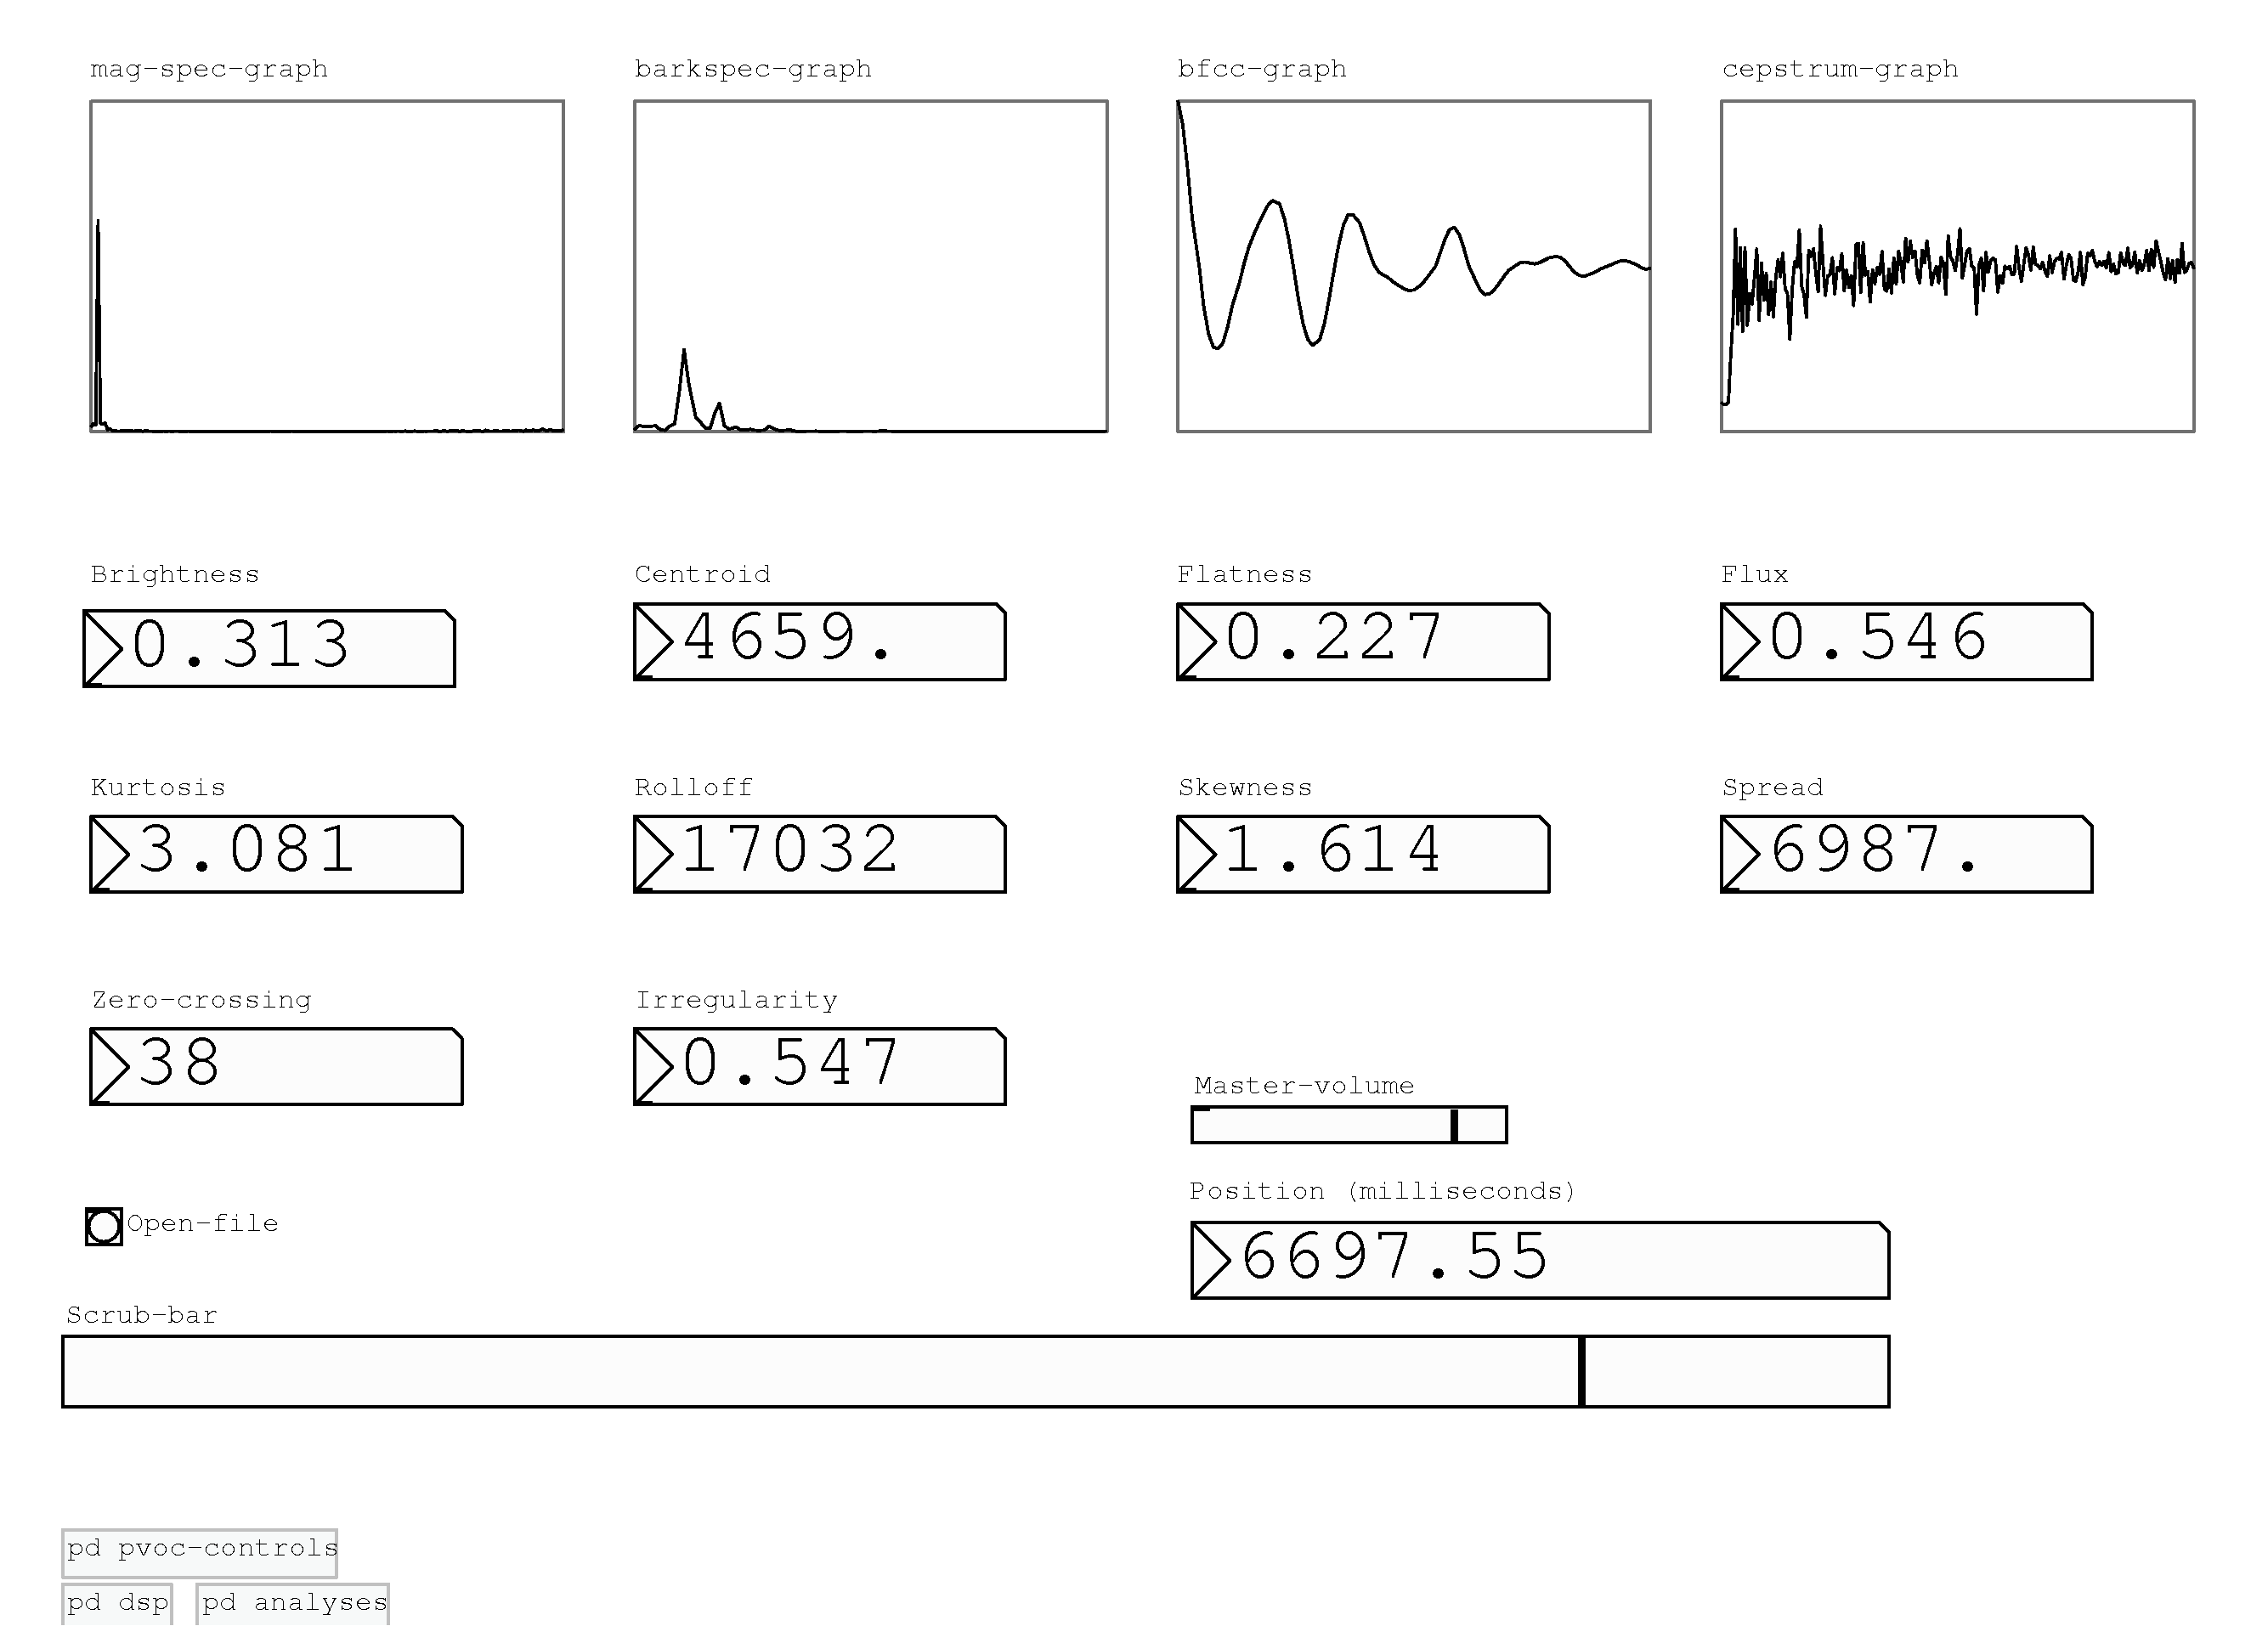
\includegraphics[scale=.75]{audio-features}
\caption{audio-features}
\label{audio-features}
\end{figure}

\begin{figure}[!h]
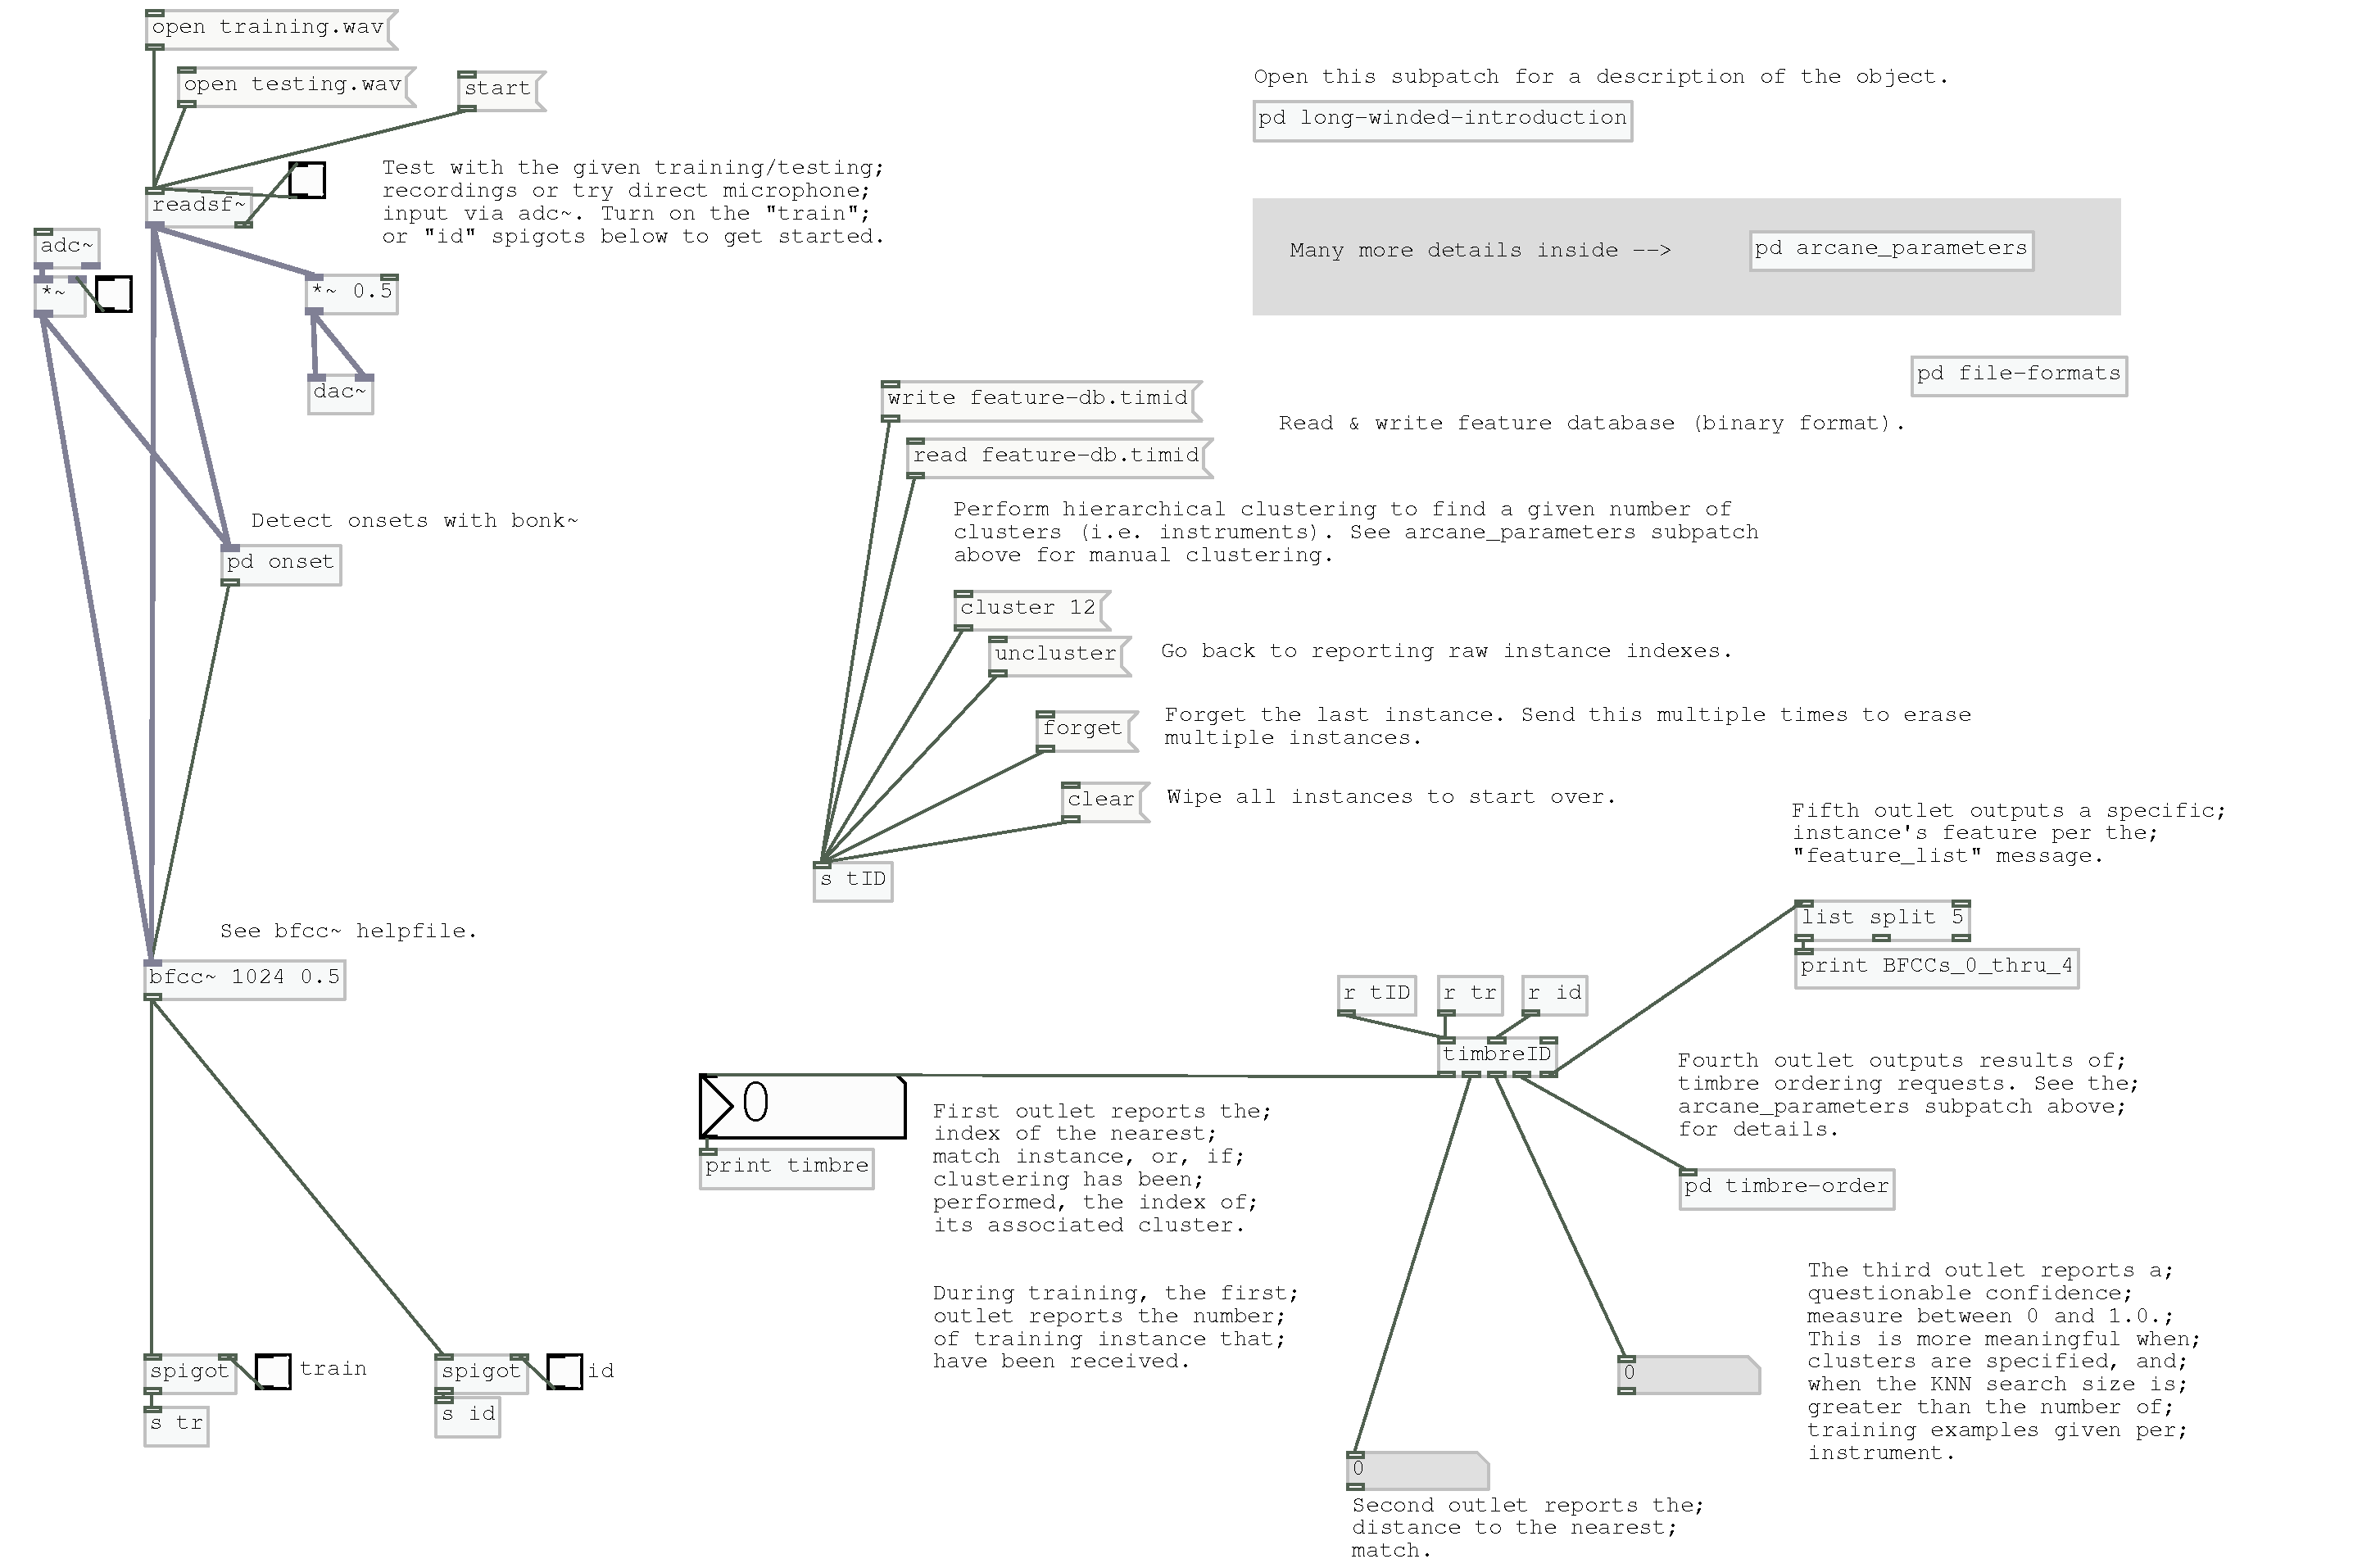
\includegraphics[scale=.75]{timbreid}
\caption{timbreID}
\label{timbreid}
\end{figure}


\begin{figure}[!h]
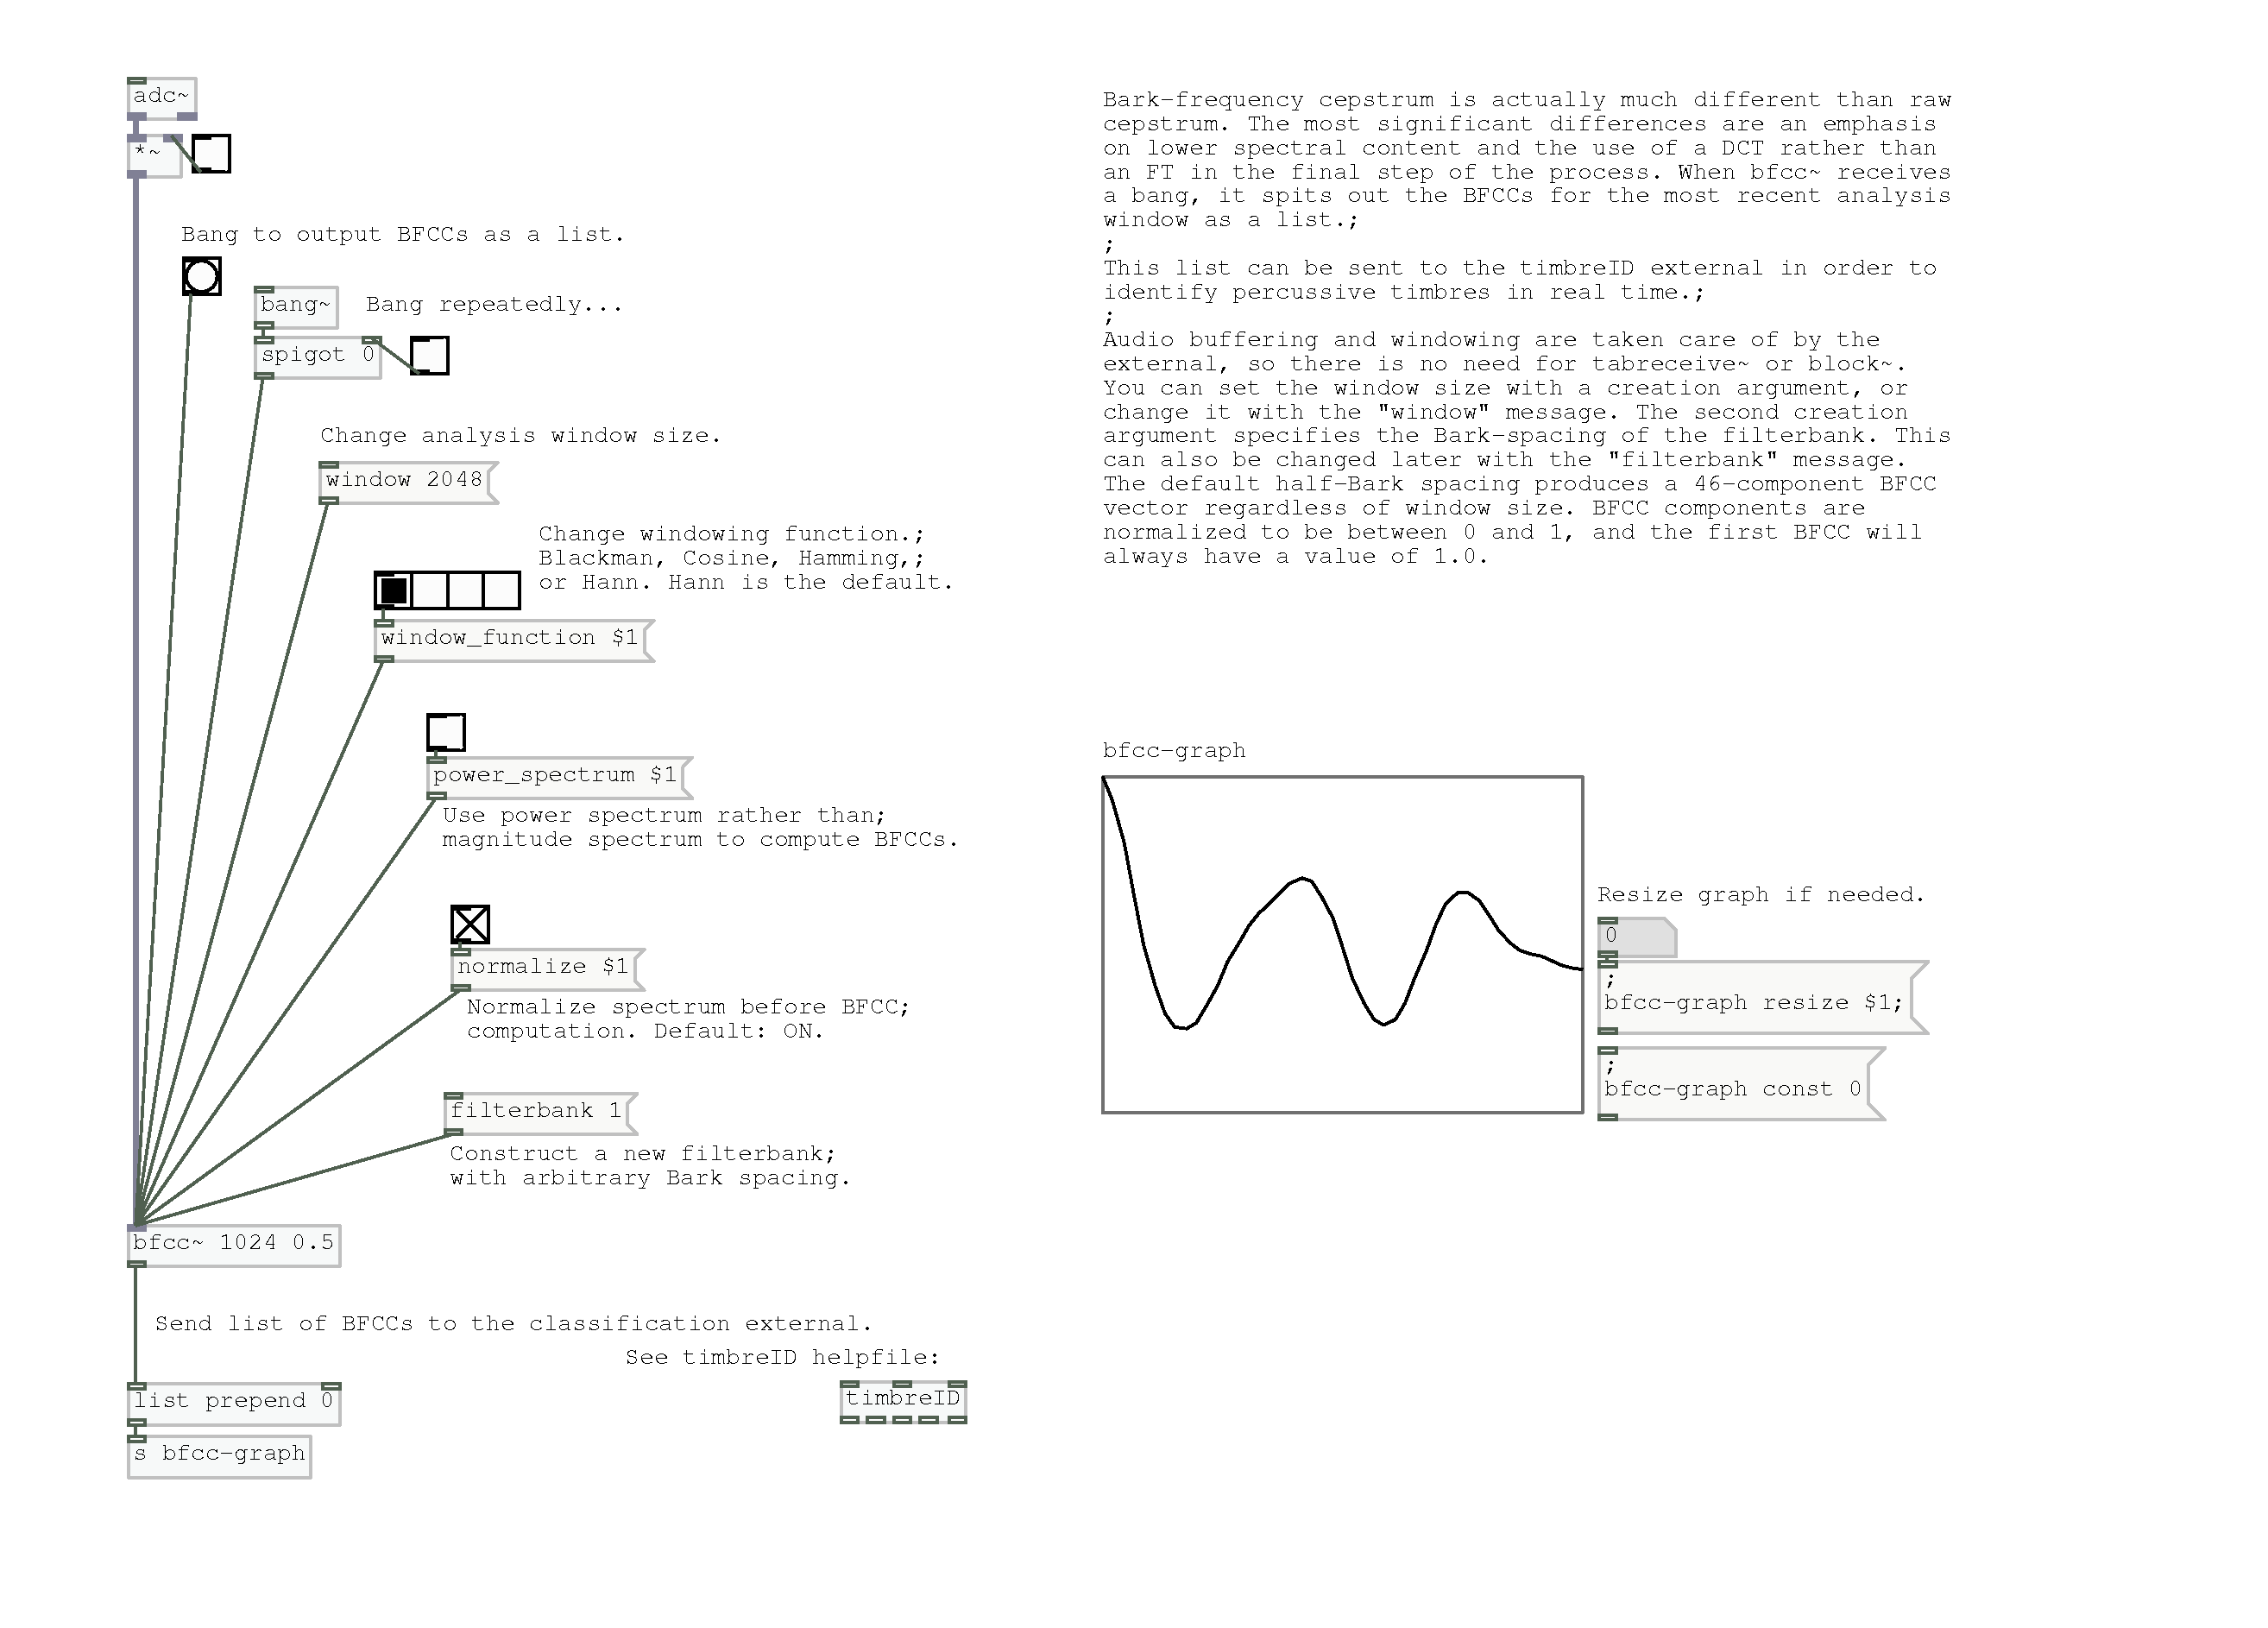
\includegraphics[scale=.75]{bfcc}
\caption{bfcc}
\label{bfcc}
\end{figure}

Quando se acessa aos dados puros da análise FFT precisamos de 
métodos específicos para filtrar esses dados. Uma densa bibliografia
tem sido desenvolvida sobre algoritmos de busca e filtragem de dados de
análise FFT. Cada algoritmo é especializado em algum aspecto, seja de
estimativa de frequência fundamental, ou de composição física da fonte sonora,
como por exemplo, estimativa do tamanho do corpo ressonante de determinada fonte.

Nese sentido, além dos dados puros da FFT feita com o objeto [rfft\texttildelow],
destacamos duas bibliitecas externas de Pd que compreendem diversos algoritmos
diferentes de análise. A primeira é a XXX desenvolvida por Adriano xxx e se tratam
de abstrações de Pd que usa apenas objetos Pd "vanilla" e por isso possui um
grande poder de compatibilidade com diversos projetos. A segunda biblioteca é a 
timbreID desenvolvida por William Brent e compreende uma série de objetos
implementados em C e possui uma boa eficácia em processamento.

Uma das vantagens da timbreID é a flexibilidade de parametrização. A biblioteca é dividida
entre objetos externos para implementação de cada algoritmo e um objeto responsável pela
classificação dos resultados dos algoritmos. O objeto de classificação (timbreID) aceita
listas de características timbrísticas e tenta encontrar a melhor correspondência entre cada 
característica do áudio de entrada e instâncias estocadas dos dados treinados.

Listas de características mandadas para a entrada da esquerda são processadas pela função
"train" (em formato de mensagem). Isso fornece exemplos das características que sobre as quais
futuras comparações serão baseadas. Uma vez que uma base de dados de treinamento é criada, ela
pode ser salva em um arquivo .timid com o método "write", e mais tarde recuperado com o método
"read". Outros formatos de saída são .txt, .mat (para uso com os programas MATLAB ou Octave)
e ARFF (para uso com o ambiente WEKA).

A segunda entrada do objeto [timbreID] recebe listas de características que são comparadas com
aquelas no banco de dados do treinamento e uma correspondência é identificada. As instâncias de 
correspondência são distinguidas pelo índice, por isso, se a correspondência mais próxima for o 
índice 7, o número 7 vai aparecer na primeira saída da esquerda.


%texto original:
% Listas de características enviadas para a terceira entrada também produz correspondências, mas esta entrada é projetada especificamente para
% síntese concatenativa . Outras mensagens que direta e restringir a pesquisa do banco de dados pode ser usado em combinação
% com esta saída. Veja o exemplo granular na [pacote exemplos timbreID] para uma explicação detalhada, e
% ouvir isso [exemplo de som] de uma voz reconstruída usando grãos a partir de um arquivo de som de instrumentos de corda friccionada.
% [Este exemplo de som] reconstrói a amostra mesma voz usando grãos a partir de um arquivo de som de ruidosos de baixa qualidade
% efeitos sonoros dos desenhos animados. Ambos os exemplos começar com apenas a voz, em seguida, desaparecer na reconstrução em tempo real granular
% da voz, então fade out a voz.
% 
% • Feature lists sent to the third inlet also produce matches, but this inlet is designed specifically for 
% concatenative synthesis. Other messages that direct and restrict the database search can be used in combination 
% with this outlet. See the granular example in the [timbreID examples package] for a detailed explanation, and 
% listen to this [sound example] of a voice reconstructed using grains from a sound file of bowed string instruments. 
% [This sound example] reconstructs the same voice sample using grains from a sound file of noisy low-quality 
% cartoon sound effects. Both examples start with just the voice, then fade in the real-time granular reconstruction 
% of the voice, then fade out the voice.
% 
% 
% 
% • Um algoritmo de clustering pode ser executado usando o "cluster" da mensagem, após o qual as instâncias serão agrupados em uma
% número desejado de clusters que representam instrumentos. Desta forma, não há necessidade de especificar exatamente quantos
% exemplos serão dados durante o treinamento. Depois de clustering, timbreID irá imprimir o índice cluster associado de
% a instância que melhor combinam com. Quando casos foram agrupados em clusters, de correspondência é realizada utilizando uma
% k-vizinhos mais próximos, estratégia, para o qual você pode especificar k. Se o cluster automática não funcionar, ou se você
% desejo de sons diferentes do grupo em conjunto, uma opção manual também está disponível.
% 
% • A tomada de quarto relatórios listas de ordenações com base em dados timbres de partida. Desta forma, você pode analisar um conjunto
% de sons e têm timbreID propor ordenações que tenham transições timbre suave. Veja o exemplo timbre ordem
% na [pacote exemplos timbreID] para uma explicação detalhada. Você também pode ouvir isso [exemplo de som] de um
% conjunto de sons reproduzidos em ordem aleatória seguido por uma ordem produzido por timbreID. Outros exemplos podem ser pedidos
% ouvido abaixo.
% 
% • pesos individuais podem ser atribuídos a característica componentes da lista. Por exemplo, se sua lista de recurso consiste em
% BFCCs e centróide, você pode peso este último a ser metade tão influente como o primeiro para calcular a distância.
% 
% • Uma vez que o tamanho da lista é arbitrária, uma forma eficaz para capturar a evolução temporal de um som é para concatenar
% os resultados da análise de múltiplas janelas sobrepostas. Esta estratégia de análise é usado no exemplo timbre ordem na
% [TimbreID pacote de exemplos], e os gráficos das análises podem ser vistas como elas ocorrem em tempo real.
% 
% 
% O recurso mais poderoso externs são baseadas na análise cepstral. cepstrum ~ saídas do cepstrum-prima de uma análise
% frame, e MFCC ~ é outra versão que distorce o resultado inicial FFT para a escala de freqüência mel. Claramente executa
% mais confiável. A técnica de MFCCs decorrentes é descrito em Rabiner \ & Fundamentos Juang de Reconhecimento de Voz.
% Em suma, todas as bandejas de FFT são executados através de um composto de sobreposição filterbank filtros triangular, ferver a
% espectro de até 20 ou mais números, que são então submetidos a uma transformada discreta de cosseno. Essa ponderação do
% eixo da freqüência pode ser mais de acordo com a forma como percebemos timbre.
% 
% bfcc ~ é o mais desenvolvido cepstral externo, utilizando a escala Bark mais profundamente pesquisados, em vez de Mels para
% a ponderação do espectro. Desempenho é apenas ligeiramente melhor do que MFCC ~. A coisa mais notável sobre essas cepstral
% externs é a flexibilidade que eles fornecem no que diz respeito à construção filterbank. A escolha de um determinado Bark ou
% mel espaçamento pode ter um impacto real sobre como as características são relevantes em classificar um conjunto de som contra outro.
% 
% Outras características espectrais no pacote são magSpec ~, barkSpec specBrightness ~, ~, ~ ~ specCentroid specFlatness,
% specFlux ~, specIrregularity ~, specKurtosis ~, specRolloff ~, specSkewness ~, specSpread ~, ~ e zeroCrossing.
% A idéia é fornecer um conjunto diversificado de ferramentas que podem ser usados ​​para pesquisa criativa na área de timbre
% classificação. Além de ser usado para criar vetores de características para enviar para o classificador timbreID, estes
% externs característica são úteis para a geração de fluxos de controle em tempo real com base no timbre.
% 
% A partir da versão 0.3.0, todos os recursos têm uma versão não em tempo real para análise de amostras carregada a arrays.
% Isso faz com que a etapa de treinamento muito conveniente para coisas como a síntese concatenativa e timbre de plotagem.
% 
% 
% 
% 
% 
% 
% • A clustering algorithm can be run using the "cluster" message, after which instances will be grouped into a 
% desired number of clusters that represent instruments. This way, there is no need to specify exactly how many 
% examples will be given during training. After clustering, timbreID will output the associated cluster index of 
% the best matching instance. When instances have been grouped into clusters, matching is performed using a 
% k-nearest-neighbor strategy, for which you can specify k. If automatic clustering doesn't work out, or if you 
% wish to group dissimilar sounds together, a manual option is available as well.
% 
% • The fourth outlet reports lists of orderings based on given starting timbres. This way you can analyze a set 
% of sounds and have timbreID propose orderings that have smooth timbre transitions. See the timbre-order example 
% in the [timbreID examples package] for a detailed explanation. You can also listen to this [sound example] of a 
% set of sounds played in random order followed by an order produced by timbreID. Other ordering examples can be 
% heard below.
% 
% • Individual weights can be assigned to feature list components. For instance, if your feature list consists of 
% BFCCs and spectral centroid, you can weight the latter to be half as influential as the former in calculating distance.
% 
% • Since list length is arbitrary, an effective way to capture the temporal evolution of a sound is to concatenate 
% analysis results of multiple overlapping windows. This analysis strategy is used in the timbre-order example in the 
% [timbreID examples package], and graphs of the analyses can be viewed as they occur in real time.
% 
% 
% The most powerful feature externs are based on cepstral analysis. cepstrum~ outputs the raw cepstrum of an analysis 
% frame, and mfcc~ is another version that warps the initial FFT results to the mel frequency scale. It clearly performs 
% more reliably. The technique of deriving MFCCs is described in Rabiner \& Juang’s Fundamentals of Speech Recognition. 
% In a nutshell, all FFT bins are run through a filterbank composed of overlapping triangular filters, boiling the 
% spectrum down to 20 or so numbers which are then subjected to a discrete cosine transform. This weighting of the 
% frequency axis may be more in line with how we perceive timbre.
% 
% bfcc~ is the most developed cepstral external, using the more thoroughly researched Bark scale rather than mels for 
% the spectrum weighting. Performance is only slightly better than mfcc~. The most noteworthy thing about these cepstral 
% externs is the flexibility they provide with respect to filterbank construction. The choice of a specific Bark- or 
% mel-spacing can have a real impact on how relevant the features are in classifying one sound set vs. another.
% 
% Other spectral features in the package are magSpec~, barkSpec~, specBrightness~, specCentroid~, specFlatness~, 
% specFlux~, specIrregularity~, specKurtosis~, specRolloff~, specSkewness~, specSpread~, and zeroCrossing~. 
% The idea is to provide a diverse set of tools that can be used for creative research in the area of timbre 
% classification. In addition to being used to create feature vectors to send to the timbreID classifier, these 
% feature externs are useful for generating real-time control streams based on timbre.
% 
% As of version 0.3.0, all of the features have a non-real-time version for analyzing samples loaded to arrays. 
% This makes the training step very convenient for things like concatenative synthesis and timbre plotting.
% 
% 
% 
% * timbreID e principais algoritmos
% 


\pagebreak 



\section{Análise Humdrum}

  Dentro de um projeto de música interativa, são necessárias informações quantitativas quanto a 
variação de parâmetros musicais pelo músico, como por exemplo quais acordes foram mais usados 
nos últimos 12 compassos.
Nesse sentido o Humdrum é uma boa plataforma de análise simbólica de estruturas musicais. 
Nesse protótipo, procuramos investigar de que maneira podem se conectar as duas linguagens 
com vizualização de dados em Gem.
Na \ref{interface} mostramos a visão geral da interface e controle
do protótipo, com a opção de se carregar um arquivo midi, 
que pode ser substituído por arquivos midi gerados em tempo real 
durante uma performance.

% \begin{figure}[!h]
% 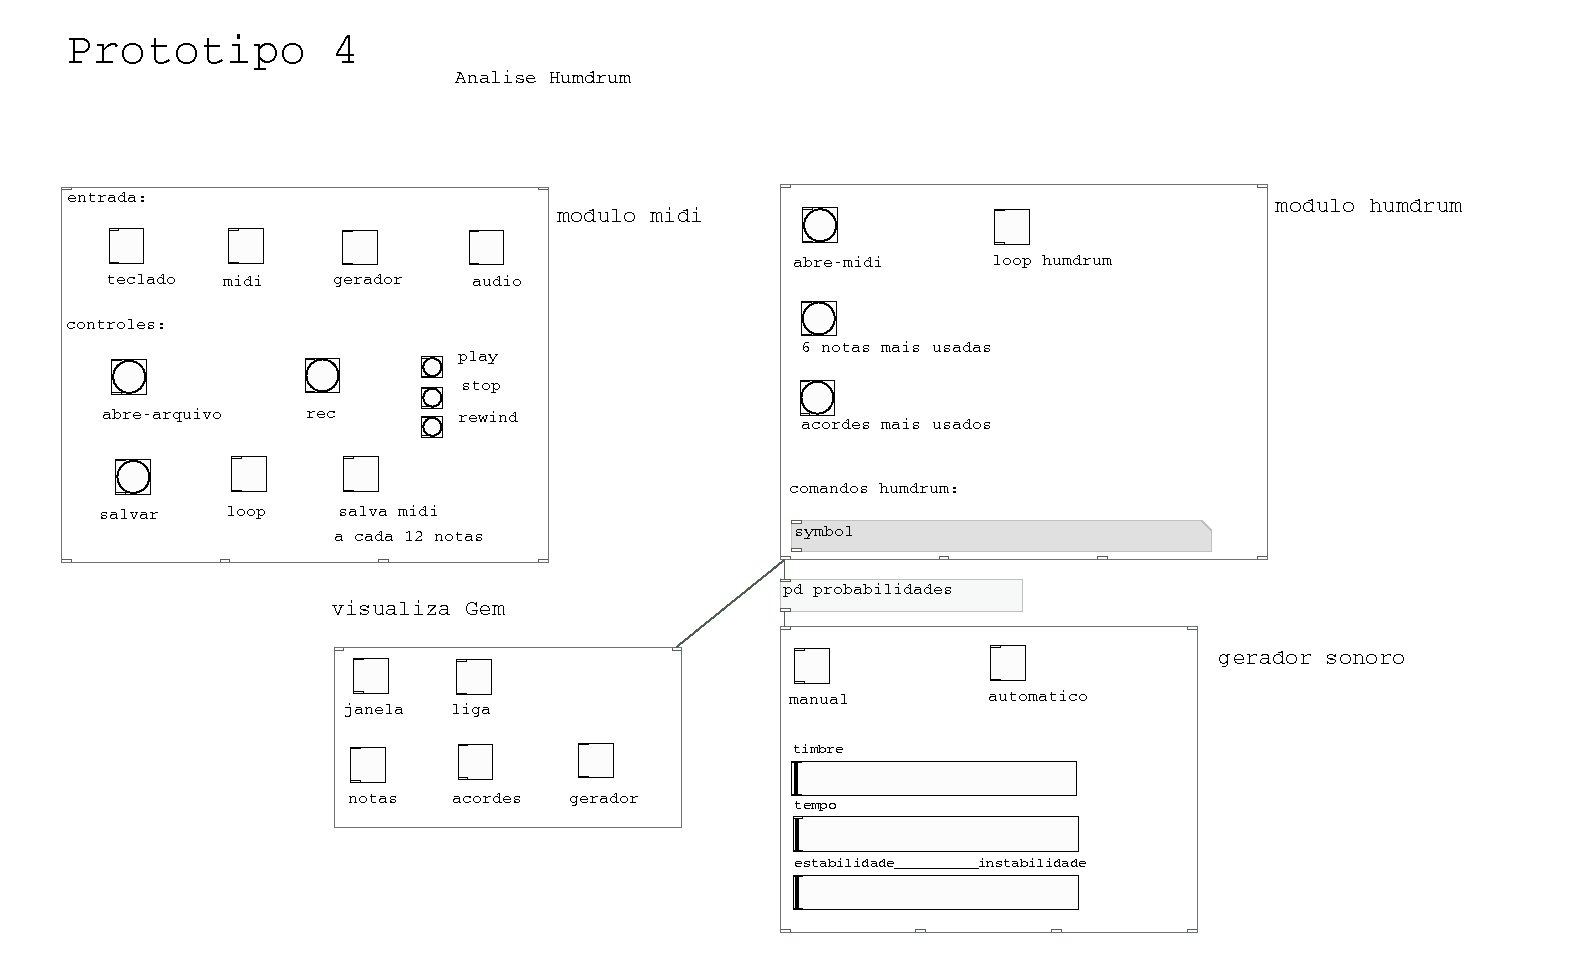
\includegraphics[scale=.5]{prot4}
% \caption{protótipo 4}
% \label{prot4}
% \end{figure}



\begin{figure}[-h]
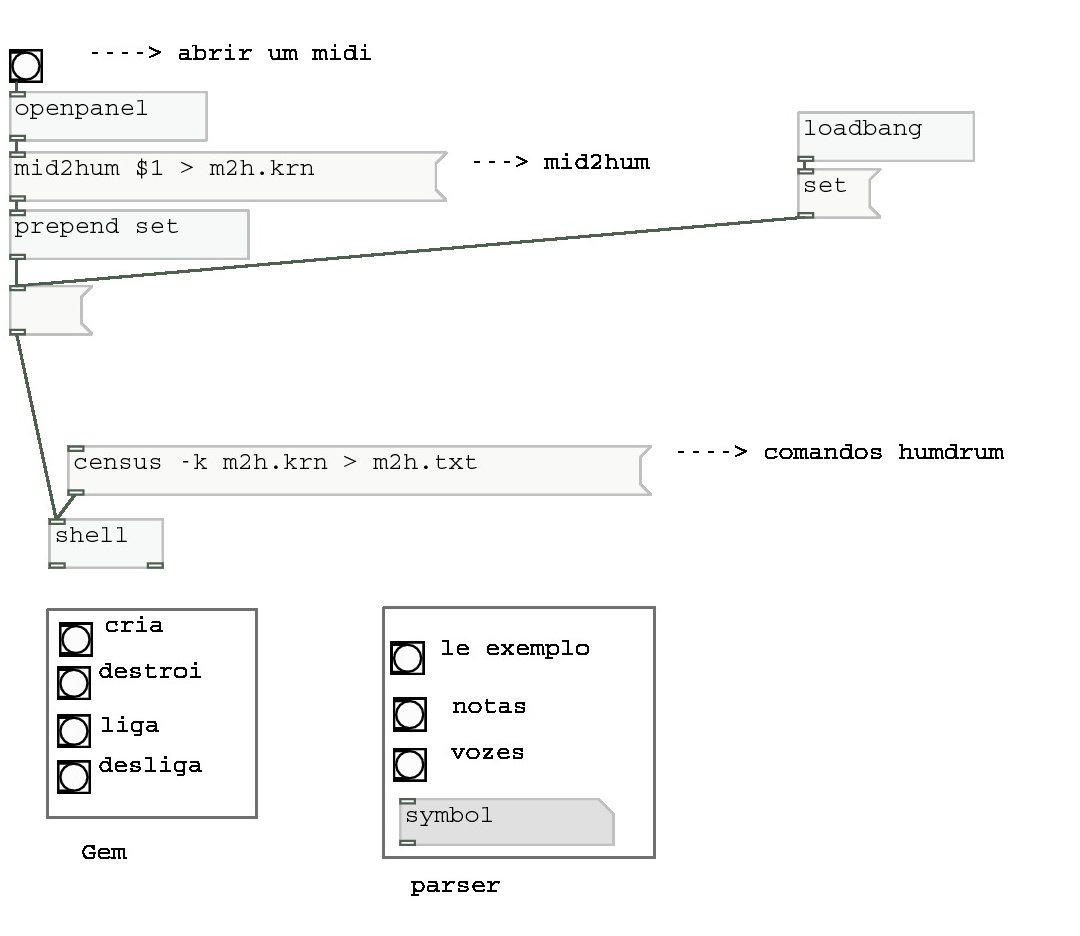
\includegraphics[scale=.7]{interface00}
\caption{interface}
\label{interface}
\end{figure} 

\textbf{Parseando strings no Pd}


O parser funciona em 3 instâncias:

1) Abre-se um arquivo midi com o objeto [openpanel] através
de uma janela de diálogo, o path do arquivo substitui a variável 
dólar 1 como argumento para o programa mid2hum que converte
arquivos midi para o formato kern (.krn), usado pelo humdrum.
\begin{verbatim}
 midi2hum $1 > m2h.krn
\end{verbatim} 
  O código acima é formatado numa mensagem e enviado ao objeto
[shell] onde converte o arquivo midi e envia o resultado para
um novo arquivo chamado m2h.krn.
 
2) Nessa etapa é onde se aplica os comandos do humdrum ao 
arquivo gerado. No caso o comando
\begin{verbatim}
census -k m2h.krn > m2h.txt
\end{verbatim} 
traz diversas informações sobre o arquivo enviadas para um 
arquivo de texto como por exemplo:
\begin{verbatim}
 HUMDRUM DATA

Number of data tokens:     2510
Number of null tokens:     0
Number of multiple-stops:  470
Number of data records:    2511
Number of comments:        817
Number of interpretations: 301
Number of records:         3629

KERN DATA

Number of note-heads:      2491
Number of notes:           2209
Longest note:              2
Shortest note:             384
Highest note:              gggg#
Lowest note:               FFF
Number of rests:           310
Maximum number of voices:  4
Number of single barlines: 237
Number of double barlines: 0
\end{verbatim} 

3) Nessa parte expomos um método de navegar e procurar por
informações no arquivo de texto. O código usado como modelo,
está assinalado na figura \ref{parser}. O arquivo m2h.txt
é lido pelo objeto [msgfile] e envia uma lista com todo conteúdo
do arquivo para os objetos [list-find] e [list-seek]. Em [list-find]
podemos procurar por um símbolo específico dentro da lista e nos retorna
a posição do símbolo. No caso do código assinalado, vemos o símbolo 
``notes:'' , porém como desejamos o valor de ``notes:'' pegamos a posição
de ``notes:'' na lista e adicionamos um número para acessar o lugar do valor de
``notes:'' na lista. Essa posição é enviada para [list-seek] que retorna o valor ou
símbolo na posição desejada. Como teste escolhemos os parâmetros ``notes:'' e ``voices:'', 
respectivamente número de notas e número de vozes encontradas no arquivo.


\begin{figure}[-h]
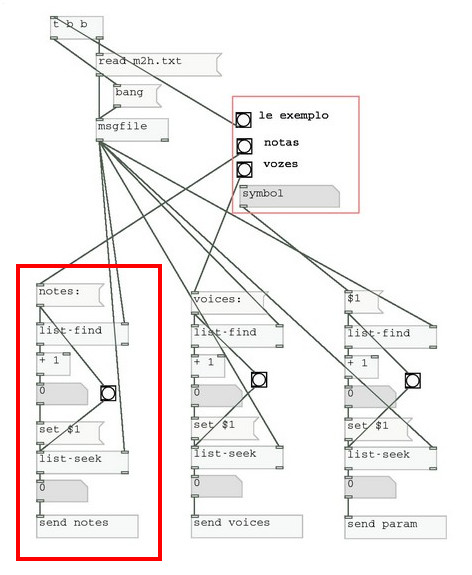
\includegraphics[scale=.5]{parser00}
\caption{parser}
\label{parser}
\end{figure} 


\textbf{Visualização com GEM}


  Os valores de números de notas e número de vozes são visualizados
com objetos da biblioteca Gem (Graphics Environment for Multimedia).
No caso os 2 parâmetros são enviados para 2 cubos 3D onde os valores
são lidos como valores de tamanho dos cubos.



\begin{figure}[-h]
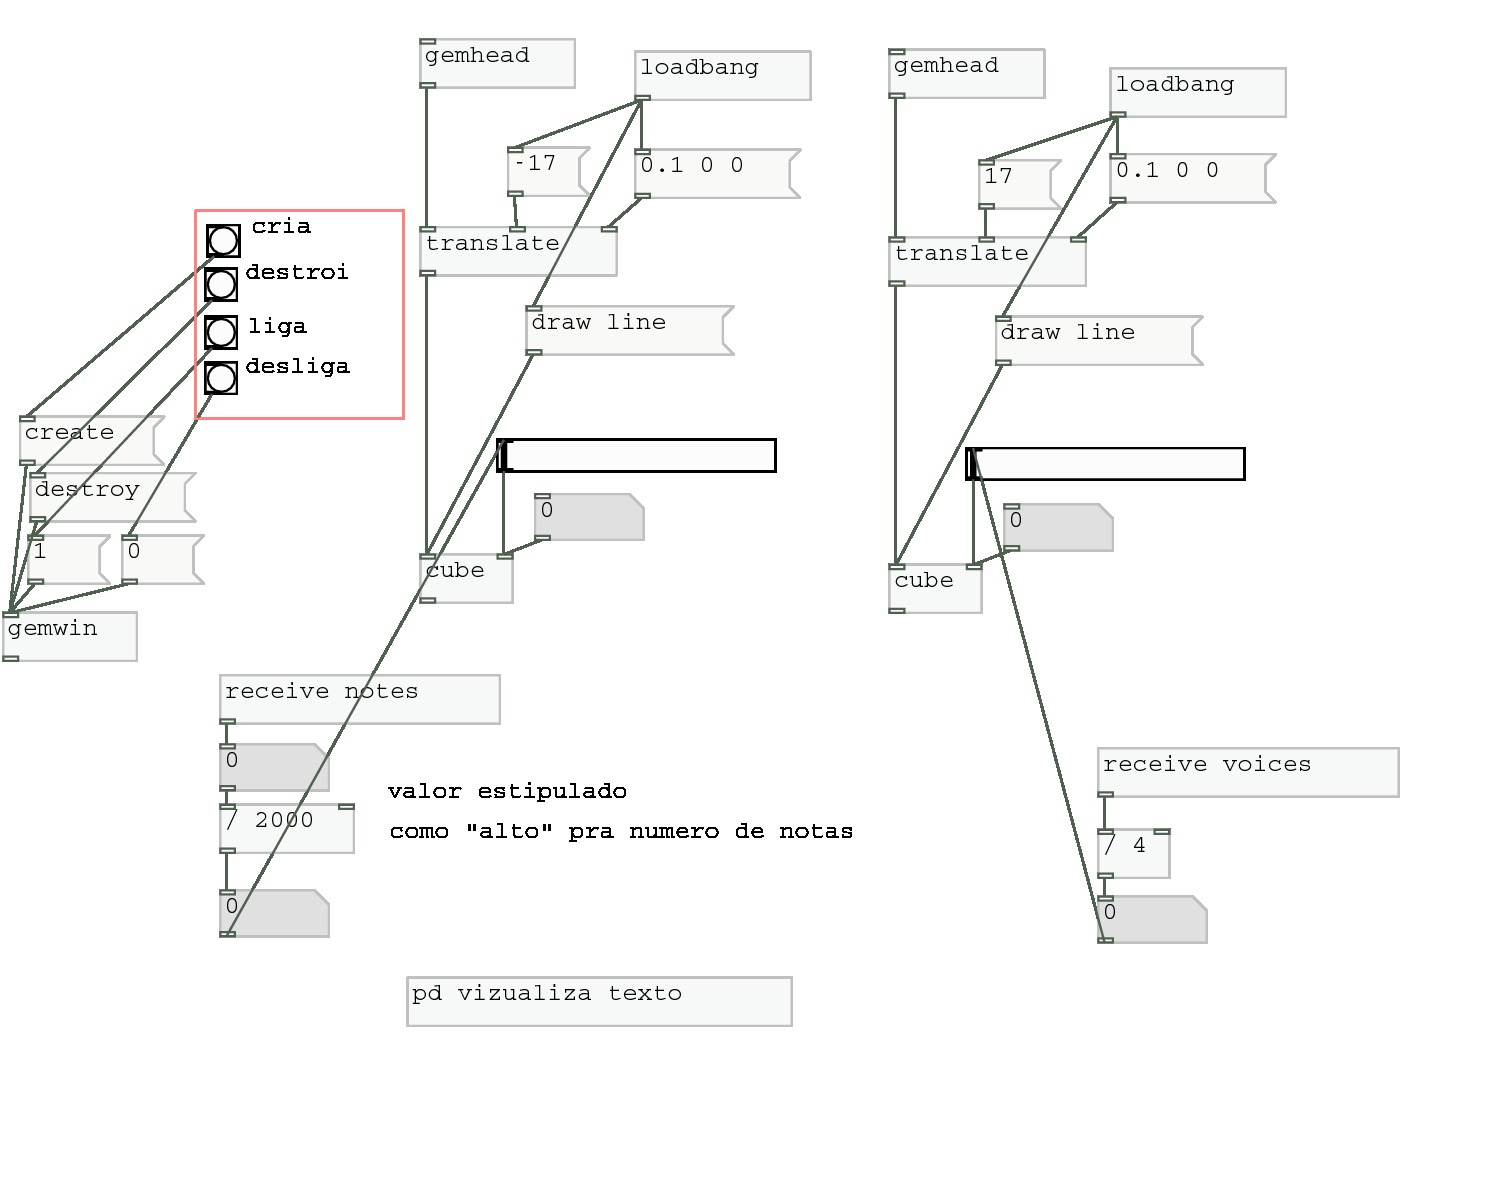
\includegraphics[scale=.5]{gem00}
\caption{GEM}
\label{GEM}
\end{figure} 


\begin{figure}[-h]
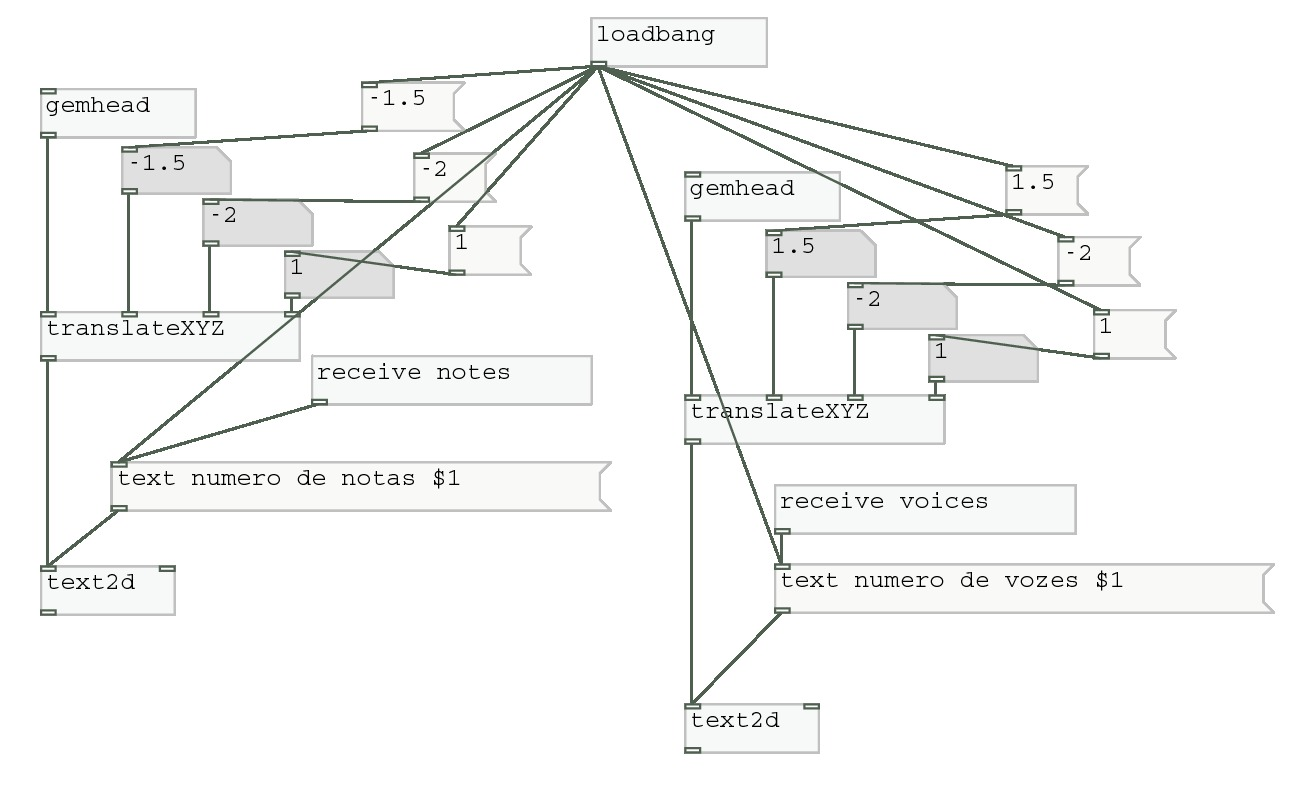
\includegraphics[scale=.5]{gemtexto00}
\caption{GEM texto}
\label{GEM texto}
\end{figure} 



\begin{figure}[-h]
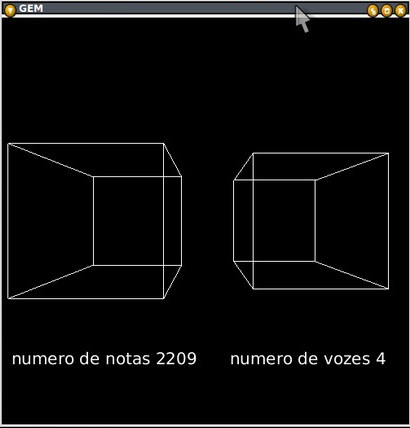
\includegraphics[scale=.5]{gemwin}
\caption{gemwin}
\label{gemwin}
\end{figure} 



  Nesse protótipo, mostramos uma metodologia
simples de unir duas linguagens muito usadas em pesquisa de música.
Essa metodologia é uma maneira clara de como acessar outra linguagem dentro do Pd
enriquecendo as possibilidades da linguagem.


\pagebreak





\section{Geradores MIDI}

Durante a implementação dos geradores de material musical,
procurou-se aliar técnicas de composição algorítmica com
o resultado das análises do áudio de entrada.


A idéia de ter uma coleção de geradores, capazes
de imitar elementos da performance humana. A análise do áudio
tenta fazer uma descrição da performance e essa descrição
é enviada aos geradores, mediados pelo cenário de interação.
Nesse sentido as análises alimentam os parâmetros dos
geradores, conduzindo o comportamento dos mesmos.



Notadamente alguns trabalhos tem influenciado bastante o desenvolvimento
dos geradores, servindo de ponto de partida para a implementação. Como
por exemplo a biblioteca RTC\footnote{A biblioteca RTC (\textit{Real-Time Composition} 
foi desenvolvida pelo compositor Karlheinz Essl em MAX, a re-implementação
em Pd foi feita por Frank Barchnet, poderemos ver uma visão mais geral
das funcionalidades dessa biblioteca no apêndice} e o método MEPSOM\footnote{
MEPSOM (Método de Ensino de Programação Sônica para Músicos) desenvolvido por
Elói Fritsch é um método que ensina composição algorítmica no ambiente MAX. Alguns
exemplos de MEPSOM foram portados para Pd e podem ser vistos no apêndice}, além
de alguns objetos das bibliotecas PDMTL e Rj.  


Músicos frequentemente separam os aspectos rítmicos, melódicos e de dinâmica
quando estudam performance ou compõe. É comum um instrumentista executar um 
mesmo perfil melódico em diferentes combinações rítmicas e com articulações
diferentes. Muitos métodos de educação musical começam com exercícios rítmicos
para depois incluir exercícios melódicos. Ao implementar os geradores midi
nessa pesquisa, levou-se em conta esses aspectos e decidiu-se manter a separação
entre os domínios do ritmo, melodia e dinâmica. Criando uma relação de funcionamento
desses geradores, possibilitando uma expansão organizada de técnicas de geração.
Na implementação de Sincopa, projetamos 3 objetos que trabalham juntos para
gerar dados midi: 

\begin{itemize}
 \item   [sinc-gera\_ritmico]
 \item   [sinc-gera\_melodico]
 \item   [sinc-gera\_dinamica]
\end{itemize}

Cada um desses objetos gerencia algumas técnicas de geração
algorítmica. É possível qualquer combinação entre esses três objetos.
A combinação entre os diversos geradores se dá na relação entre a 
análise do áudio de entrada e a escolha de um cenário de interação. 

A manipulação de dados midi compreende algumas técnicas bem estabelecidas
no Pd. A geração de notas midi é realizada com o objeto [makenote] que formata
dados de entrada em notas midi, fornecendo as mensagens "noteon" e "noteoff", baseado
no valor de duração. As entradas e saídas midi são feitas com os objetos
[notein] e [noteout] respectivamente. O objeto [seq] grava e manipula arquivos 
do tipo midi, porém, os parâmetros das mensagens midi podem ser facilmente escritos
em arrays e listas para então serem manipulados.

\begin{figure}[!h]
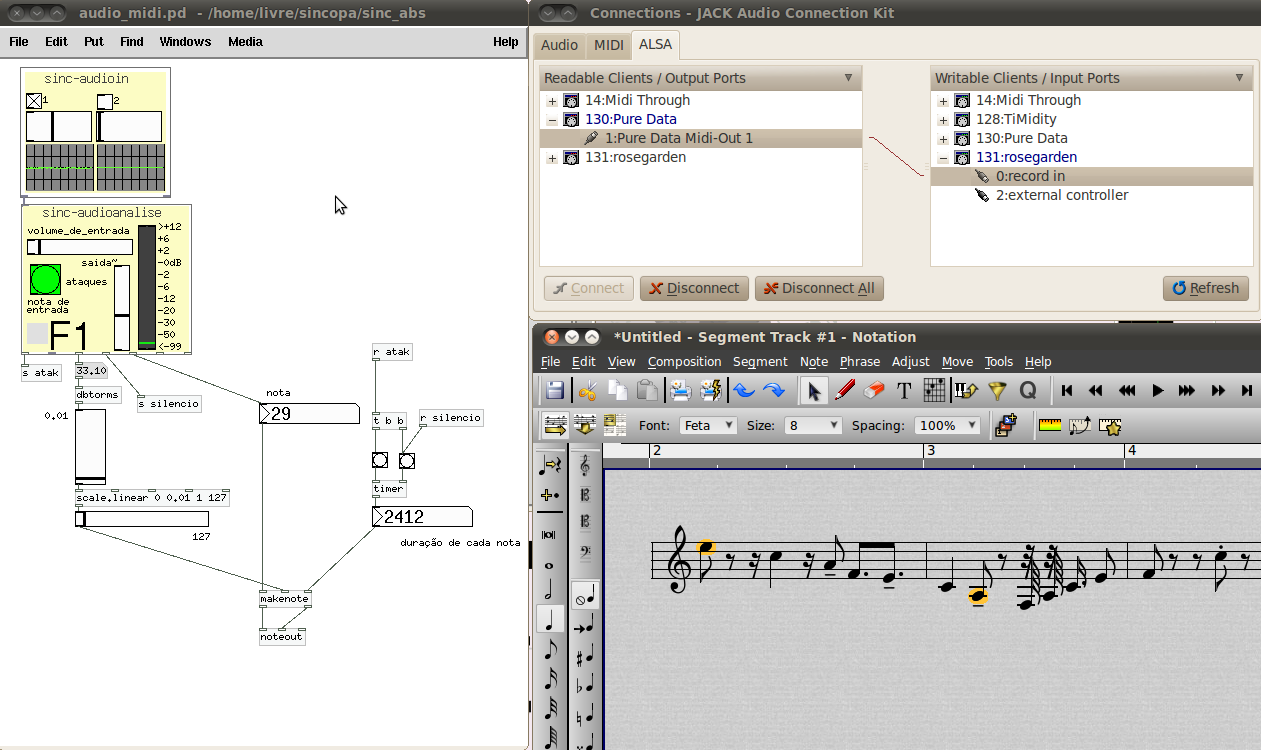
\includegraphics[scale=.5]{audio2midi}
\caption{Conversão de áudio para notas midi}
\label{audio2midi}
\end{figure}


Na figura \ref{audio2midi} vemos no patch a esquerda, o fluxo de entrada de áudio do objeto
[sinc-audioin], sendo analisado pelo objeto [sinc-audioanalise] e posteriormente
sendo convertido para mensagens midi com auxílio dos objetos [makenote] e [noteout].
Podemos observar ainda a dinâmica sendo convertida de decibéis (distribuição exponencial)
 para RMS (distribuição linear) com o objeto [dbtorms]. Após essa conversão,
o valor da dinâmica é convertido para uma escala midi de 0 a 127. Para isso é usado
o objeto [scale.linear] da biblioteca "pdmtl". O valor de duração das notas é determinado
pelo objeto [timer] que recebe uma mensagem (bang) a cada detecção de ataque e de silêncio.
No panorama geral da figura\ref{audio2midi} vemos o Pd mandando mensagens midi em tempo-real
para o programa Rosegarden, usando conexão midi do programa Jack. 


\subsection{Geradores rítmicos}






\begin{figure}[!h]
\includegraphics[scale=.5]{sinc-gera_ritmo}
\caption{Objeto [sinc-gera\_ritmico]}
\label{[sinc-gera_ritmico]}
\end{figure}

No atual estágio da pesquisa, foi implementada uma abstração gráfica
que gerencia a atividade de quatro geradores rítmicos. Dessa
maneira se torna fácil de administrar durante uma performance
e também se mantém a flexibilidade de expandir para quantos
geradores diferentes se queira. A interface pode ser vista na figura \ref{[sinc-gera_ritmico]}


\subsubsection{Gerador rítmico imitativo}



\begin{figure}[!h]
\includegraphics[scale=.6]{gerador_ritmico0}
\caption{subpatch [pd gerador-ritmico0] de [sinc-gera\_ritmico]}
\label{gera_ritmico0}
\end{figure}   


No patch da figura \ref{gera_ritmico0} vemos um gerador de



% \item
 \subsubsection{Ritmo baseado em variações}


Na figura \ref{gera_ritmico1} vemos um gerador rítmico
que compõe novas sequências rítmicas a partir de variações
da tabela de durações.

Essas variações podem ser:

\begin{figure}[!h]
\includegraphics[scale=.6]{gerador_ritmico1}
\caption{Gerador rítmico baseado em probabilidades de durações}
\label{gera_ritmico1}
\end{figure}  




% \item
 \subsubsection{Movimento browniano como gerador de durações}


\begin{figure}[!h]
\includegraphics[scale=.6]{gerador_ritmico2}
\caption{Gerador rítmico baseado em movimento browniano}
\label{gera_ritmico2}
\end{figure}  


O terceiro gerador é mostrado na figura \ref{gera_ritmico2} e
realiza uma combinação entre os objetos [tabletool] e [brown-rhythm].

O objeto [tabletool]\footnote{Objeto externo desenvolvido em C
por William Brent e compilado e testado no ambiente de desenvolvimento
dessa pesquisa} permite que se façam operações matemáticas
recursivas e análise em arrays de números. 

Nesse caso, [tabletool] é responsável por informar os valores
mínimo e máximo de durações de tempo entre notas, que estão
armazenados no array \textit{\$0-ritmo\_manip}, enviando
esses respectivos valores como variáveis [s min\_ritmo] e 
[s max\_ritmo] para o gerador de durações [brow-rythm].


 \begin{figure}[!h]
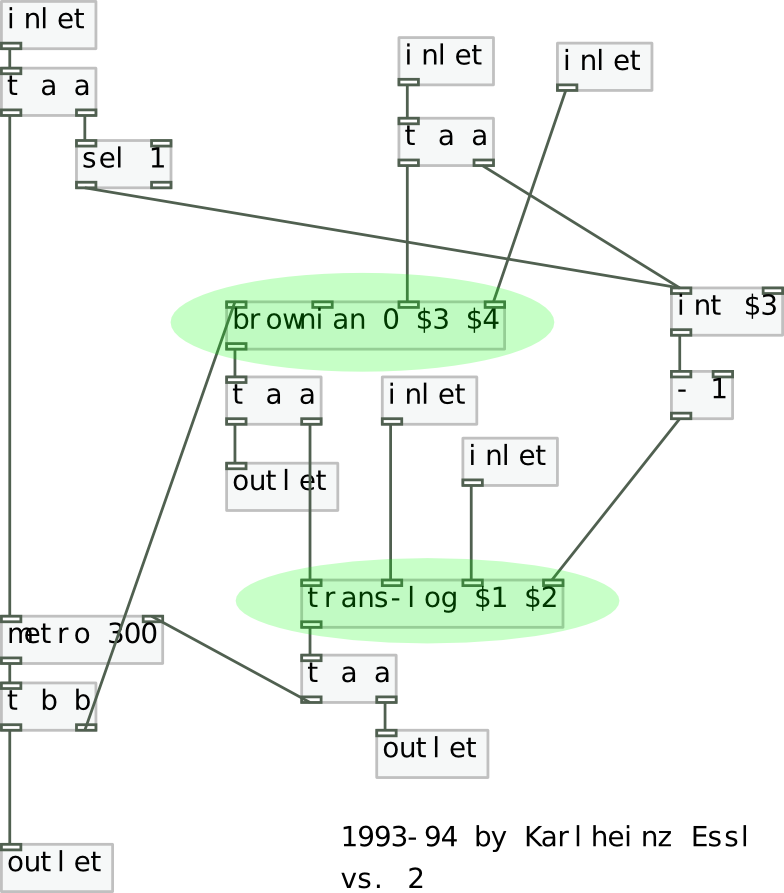
\includegraphics[scale=.6]{brown-rythm}
\caption{brow-rythm}
\label{brown-rythm}
\end{figure}  

O objeto [brown-rhythm] está presente na biblioteca RTC e se trata de
um gerador de durações baseado em movimento browniano("Brown motion"
\footnote{movimento browniano é um modelo que descreve o movimento aleatório 
de partículas macroscópicas num fluido como consequência dos choques das 
moléculas do fluido nas partículas. Esse nome é devido ao botânico Robert
Brown, que observou minúsculas partículas dentro dos vacúolos dos grãos de 
pólen executando um movimento agitado. Repetindo o experimento com partículas de poeira, 
ele foi capaz de definir que o movimento se deu devido às partículas estarem "vivas", 
embora a origem do movimento ainda estivesse para ser explicada.
O cientista que explicou corretamente esse movimento, propondo que a energia fosse 
constituída de partículas, foi Albert Einstein, em 1905.
Movimento browniano é um dos modelos mais usados de processos estocásticos
(ou probabilísticos) sobre tempo contínuo.} )

 \begin{figure}[!h]
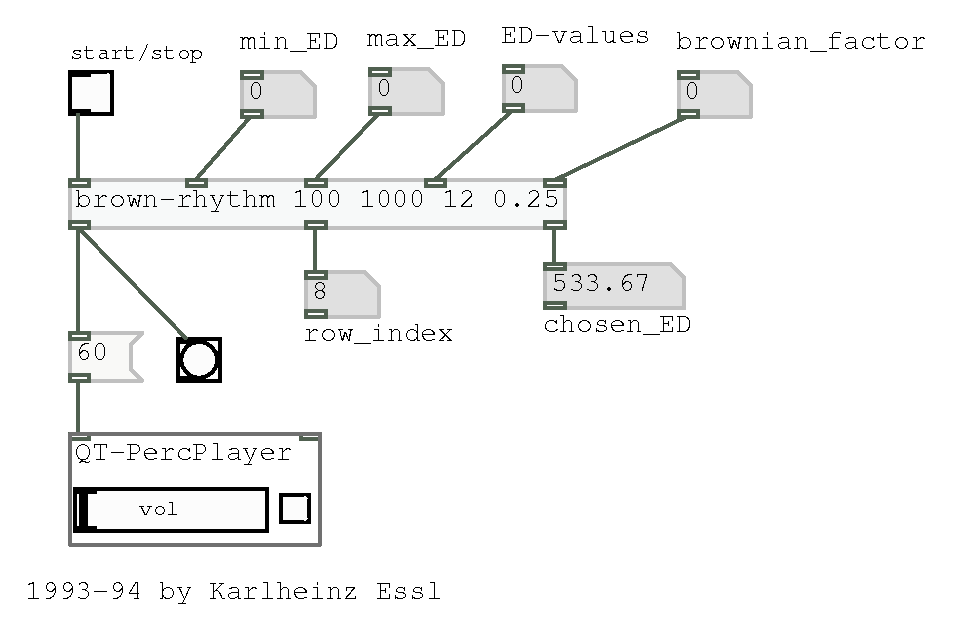
\includegraphics[scale=.6]{brown-rhythm-func}
\caption{Funcionamento básico de [brow-rhythm]}
\label{brown-rythm-func}
\end{figure} 


O funcionamento básico aparece na figura \ref{brown-rhythm-func}.
No manual de [brown-rhythm] aparece uma explicação mais detalhada.


\begin{quote}
Generates a brownian-movement-like rhythm of a geometrical row of
entry delays (ED) and a certain number of ED-values. The brownian factor
determines the distance between two succeding rhythmical values. A factor
of 0 produces a periodic rhythm, where a factor of 1 output random values 
of the given range.
\end{quote}  



Na figura \ref{brown-rythm} vemos como [brown-rythm] é construído internamente.
Nota-se em destaque os principais objetos envolvidos na construção
de [brown-rhythm]. Basicamente, o objeto [brownian] é uma implementação de
distribuição de Brown no Pd. E [trans-log] é um objeto que realiza uma
transição logarítmica entre números.

 \begin{figure}[!h]
\includegraphics[scale=.6]{brownian_func}
\caption{Funcionamento de [brownian]}
\label{brownian_func}
\end{figure} 

Podemos ver o funcionamento básico do objeto [brownian] acessando seu
manual (figura \ref{brownian_func}.  A saída desse objeto retorna números randômicos entre o mínimo
(''min'' (int, float)) e o máximo (''max" (int, float)). A distância entre
dois números randômicos é determinada pelo fator de brown (float
entre 0 e 1). Quando esse fator é 1, [brownian] se comporta como um
gerador randômico ordinário (objeto [random] por exemplo). Quando
o fator é 0, o mesmo número sempre é repetido.


\begin{figure}[!h]
\includegraphics[scale=.6]{brownian_exemplo}
\caption{objeto [brownian] com diferentes valores de fator de brown}
\label{brownian_exemplo}
\end{figure} 

É possível comparar diferentes comportamentos de [brownian] observando
a figura \ref{brownian_exemplo}, onde vemos três objetos [brownian] com
os mesmos parâmetros de inicialização, cada um escrevendo os resultados
em diferentes arrays de 50 elementos. A única diferença entre os 3 está 
no fator de brown, assinalado em rosa (0.01 , 0.1 e 0.5 respectivamente).
Musicalmente, um baixo fator de brown aplicado a durações entre notas
possibilita a emergência de padrões rítmicos bem estabelecidos com 
pequenas variações. Quando aumentamos gradualmente o fator de brown, ouvimos
uma transição rumo a uma instabilidade rítmica e a quebra de padrões. 
O objetivo desse gerador é se aproximar da performance do músico real.
O objeto [sinc-audioanalise] analise o áudio de entrada estimando os valores de duração entre notas.
Esse valores são enviados a [sinc-calc\_ritmo] que faz uma estimativa do grau
de instabilidade, como explicado na página \ref{[sinc-calc_ritmo]} (como faz pra ref a página?).
O grau de instabilidade rítmica influencia direto o comportamento do fator de brown, de acordo
com a definição do cenário de interação a que se propõe. O cenário pode definir, por exemplo, que
um ritmo estável do músico (baixa instabilidade), provoque um comportamento rítmico instável
do gerador (fator de brown alto).



 \begin{figure}[!h]
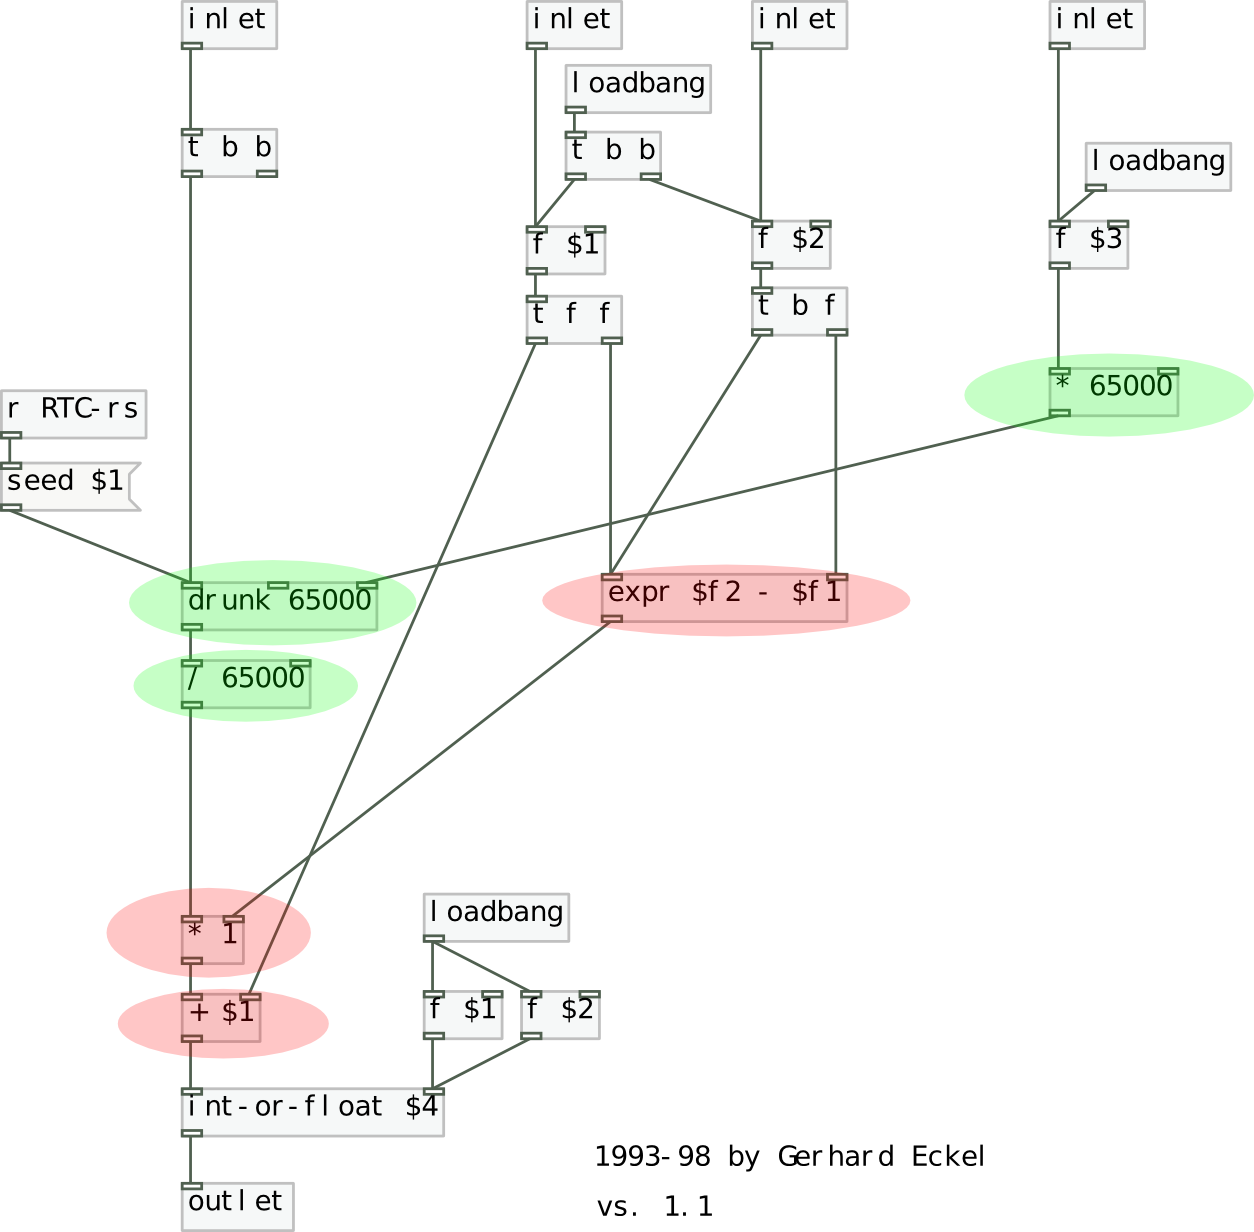
\includegraphics[scale=.6]{brownian}
\caption{[brownian]}
\label{brownian}
\end{figure} 


Na figura \ref{brownian} vemos a composição interna do objeto [brownian] onde temos elementos
grifados com a cor verde e outros com a cor rosa. Se trata de duas partes
distintas do patch, a parte com a cor verde, representa o controle dos
parâmetros do objeto [drunk] que é a implementação de um modelo de \textit{random-walk}
no Pd. A área destacada em rosa mostra uma sequência de objetos que 
escalonam o resultado dentro da amplitude de valor mínimo (\$1) e máximo (\$2).

 \begin{figure}[!h]
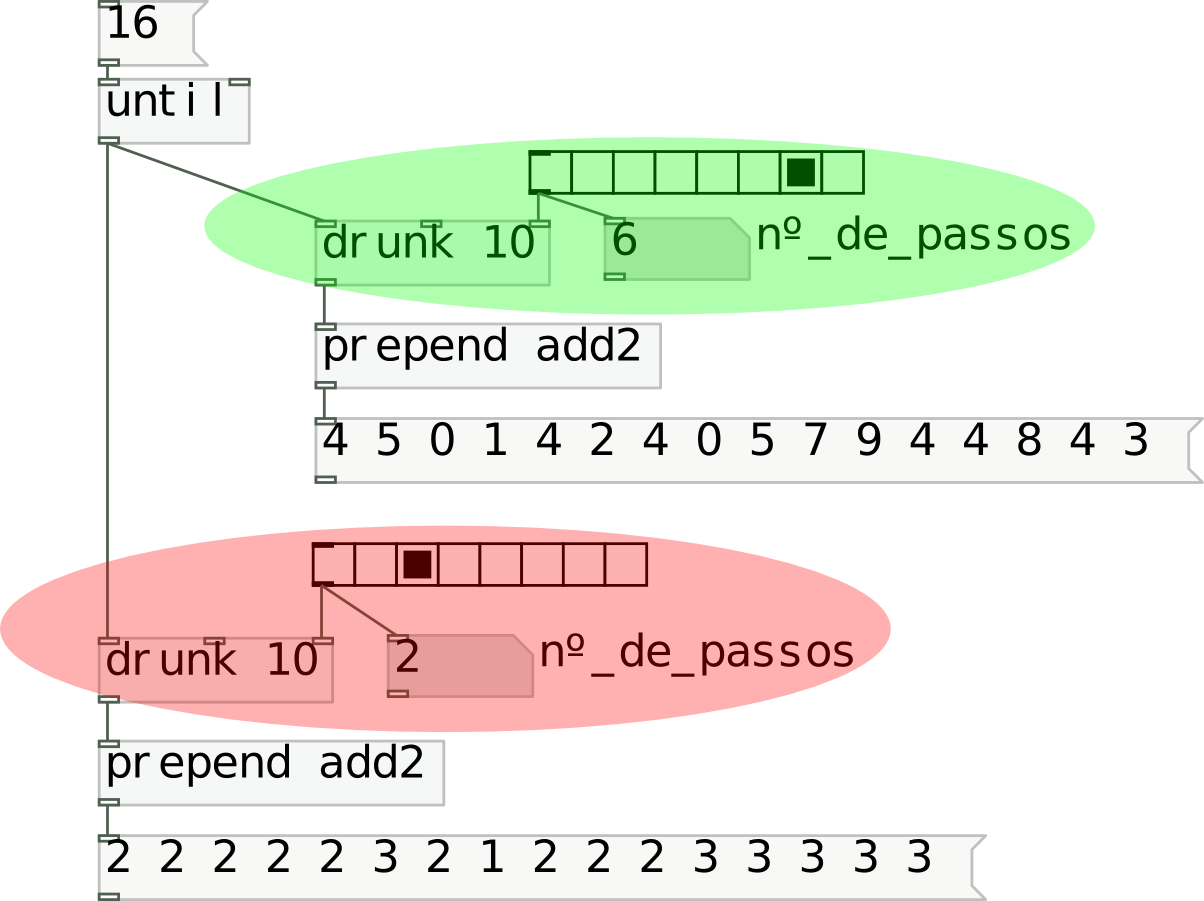
\includegraphics[scale=.6]{drunk}
\caption{exemplo de funcionamento de [drunk]}
\label{drunk}
\end{figure} 

O objeto [drunk] pertence a biblioteca Cyclone, que tem como objetivo
implementar objetos compatíveis entre Pd e MAX. O objetivo de [drunk] é
retornar números randômicos dentro de uma escala variável. A distância
entre cada número randômico é definida pelo valor da terceira entrada
de [drunk]. Essa variável define o maior número de passos possível entre 
dois resultados de [drunk]. Podemos ver na figura \ref{drunk} que temos
dois objetos [drunk] sorteando 16 valores de 0 a 10 com a diferença do
número de passos, com 6 (destaque em verde) e 2 (destaque em rosa).

Os objetos [brownian] e [drunk] são muito úteis para a composição 
interativa por permitirem a variação dos parâmetros do algoritmo
em tempo-real. Essa funcionalidade é usada em SINCOPA em outros geradores
melódicos e de dinâmica.


%  \item
\subsubsection{Gerador rítmico polifônico}


\begin{figure}[!h]
\includegraphics[scale=.6]{gerador_ritmico3}
\caption{Gerador rítmico randômico}
\label{gera_ritmico3}
\end{figure}  

O gerador da figura \ref{gera_ritmico3} é baseado no 
objeto [repchord-rhythm] da biblioteca RTC. O objetivo desse objeto é 
ter um gerador com capacidade de controle dos parâmetros da polifonia.

O objeto [repchord-rhythm] é um gerador rítmico polifônico cujas taxa repetição
e densidade do acorde são dependentes dos graus de periodicidade de durações
mínima e máxima entre notas. 
%\end{itemize}


\subsection{Geradores melódicos}


Da mesma maneira que os geradores rítmicos.....
No atual estágio da pesquisa, foi implementada uma abstração gráfica
que gerencia a atividade de quatro geradores melódicos. Dessa
maneira se torna fácil de administrar durante uma performance.
E também se mantém a flexibilidade de expandir para quantos
geradores diferentes se queira.


De maneira geral, os geradores melódicos dependem dos geradores
rítmicos. Os geradores rítmicos "pedem" nota por nota para o geradores
melódicos


\begin{figure}[!h]
\includegraphics[scale=.45]{sinc-gera_melodico}
\caption{Abstração que organiza 4 geradores melódicos}
\label{[sinc-gera_melodico]}
\end{figure}


\subsubsection{Melodia imitativa}

Nesse primeiro gerador melódico o método de geração
é a leitura linear da tabela temporária de pitches
como se pode ver na figura \ref{gera_melodico0}.


\begin{figure}[!h]
\includegraphics[scale=.6]{gera_melodico0}
\caption{[pd gerador-melodico0]}
\label{gera_melodico0}
\end{figure}  

\begin{figure}[!h]
\includegraphics[scale=.55]{gera_mel0}
\caption{exemplo de melodia imitativa gerada}
\label{gera_mel0}
\end{figure}  




O objetivo desse gerador é a imitação melódica
do instrumentista.

\subsubsection{Melodia de probabilidades}



Nesse objeto foi implementada uma probabilidade unidimensional
de durações. Ou seja, o valor absoluto de cada duração
da performance do músico alimenta uma tabela de durações.
Uma possível aplicação seria a aplicação de probabilidades de 
padrões maiores de durações. Permitindo a recorrência dos padrões
rítmicos que emergem ao longo da performance.


No Pd podemos implementar um sistema simples de probabilidade como 
vemos na figura XXX

% fazer exemplo simples de probabilidade genérica - patch simples



O objeto [probalizer], simplifica o trabalho.

Importância das probabilidades serem atualizadas em
tempo-real.

Explicar patch simples de probabilidade e como
seria a re-implementação do probalizer apenas com vanilla.


O gerador melódico da figura \ref{gera_melodico1}, é baseado
no objeto gráfico [probalizer] da biblioteca "Unauthorized"
distribuída com o pd-extended.

O objeto [probalizer], facilita o trabalho.

Importância das probabilidades serem atualizadas em
tempo-real.
Explicar probabilidade simples.

\begin{figure}[!h]
\includegraphics[scale=.6]{gera_melodico1}
\caption{[pd gerador-melodico1]}
\label{gera_melodico1}
\end{figure}  

\subsubsection{Movimento browniano como gerador melódico}


\begin{figure}[!h]
\includegraphics[scale=.6]{gera_melodico2}
\caption{[pd gerador-melodico2]}
\label{gera_melodico2}
\end{figure}  


O terceiro gerador é mostrado na figura \ref{gera_melodico2} e
realiza uma combinação entre os objetos [tabletool] e [brown-melody].


\subsubsection{Melodia  de notas randômicas}


\begin{figure}[!h]
\includegraphics[scale=.6]{gera_melodico3}
\caption{[pd gerador-melodico3]}
\label{gera_melodico3}
\end{figure}  

O gerador da figura \ref{gera_melodico3} é baseado no 
objeto [random.integer]. O objetivo desse gerador é 
ter um gerador com alto grau de permeabilidade melódica.

\subsection{Geradores de amplitudes}

São encontrados diferentes termos definindo o aspecto
da amplitude sonora como dinâmica (quando nos referimos a notação tradicional),
velocity (quando se refere a dados MIDI), volume e amplitude (mais
usado quando se refere a descrição física da onda sonora).


As variações de amplitude podem produzir diferentes gestos musicais,
Gerando acentos, diferentes articulações...


\subsubsection{Amplitude imitativa}

bla bla bla

\subsubsection{Gerador de amplitude baseado em variação}

\subsubsection{Movimento browniano como gerador de amplitude}

\subsubsection{Amplitude polifônica}


\subsection{Harmonizador automático}

\subsubsection{Nota pertence ao acorde}
%% antigo::


O protótipo 2 tem como objetivo apresentar possibilidades de harmonização automática em tempo-real,
onde o sistema tendo o conhecimento da linha melódica criada instantaneamente pelo músico, consegue
harmonizar essa linha melódica, tendo como a maior exigência que o acorde contenha a nota que está sendo
tocada. Para isso são expostas 4 possibilidades de harmonização automática, com resultados distintos.

No patch da figura \ref{harm1}  temos a célula básica do harmonizador diatônico (modo 1)
 usado no protótipo. 
O objeto [receive fiddle] recebe o fluxo de notas e o objeto [decide], escolhe 
randomicamente quais notas vão ser harmonizadas, e manda sua decisão para o objeto 
[spigot] que funciona como uma chave seletora liberando ou não a nota para ser harmonizada. 
Após a nota ser liberada para o harmonizador, vai acontecer  a escolha de qual acorde será 
sobreposto a essa nota. Isso é feito pelo objeto [random 4] que escolhe randomicamente um 
número de 0 a 3, cada um representando uma operação a ser feita com a nota dada pela flauta 
(ver ainda na figura \ref{harm1} - ``tabela de resultados de [random 4]'').

\begin{figure}[!h]
\includegraphics[scale=.6]{harm1}
\caption{Decisão de qual nota a ser harmonizada}
\label{harm1}
\end{figure}

\begin{figure}[!h]
\includegraphics[scale=.6]{harm2}
\caption{sub-patch ``pd tonica''}
\label{harm2}
\end{figure}

\begin{figure}[!h]
\includegraphics[scale=.4]{harm3}
\caption{resultado da harmonização com modo 1}
\label{harm3}
\end{figure}


Na figura \ref{harm2} podemos ver o que acontece dentro do sub-patch [pd tônica], onde a nota sorteada 
será a tônica de uma tríade maior ou menor dependendo do resultado de [random 2]. A figura \ref{harm3} 
mostra um pequeno exemplo dos resultados desse harmonizador. Nesse exemplo, a primeira nota 
harmonizada é um si que virou terça maior de uma tríade maior. Um aspecto interessante desse 
harmonizador é que mesmo em exemplos curtos quase sempre se chega a relações de mediantes 
cromáticas, como é o caso do terceiro e quarto acordes (Mib - Lab), nesse caso uma relação 
enarmônica de mediante cromática.

\begin{figure}[!h]
\includegraphics[scale=.5]{harm4}
\caption{harmonizador dissonante , modo 2}
\label{harm4}
\end{figure}

Apesar de muitas vezes os acordes gerados pelo harmonizador diatônico possuírem uma relação 
cromática, todos os acordes gerados são tríades maiores ou menores. Para criar um contraste 
criei um harmonizador de acordes alterados que está na figura \ref{harm4}. Nesse harmonizador todas notas 
que entram são tônicas e todas são harmonizadas. 
	A escolha do acorde para cada nota é feito através de distribuição de probabilidade, 
arranjado com o objeto [moses]. Quando uma nota entra, ela gera randomicamente um número de 0 
a 99 com o objeto [random 100], esse valor então é endereçado a um dos quatro tipos de tétrades 
possíveis nesse patch : aumentado com 7ª menor, alterado com 5ª diminuta (6ª aumentada Francês), 
menor com sétima maior ou maior com sétima maior. Cada uma das quatro tétrades tem 25 por cento 
de probabilidade de aparecer. Cada membro dos acordes é endereçado a um gerador de síntese aditiva 
com amplitude bem baixa. Em função da amplitude bem baixa do harmonizador de acordes alterados, o 
resultado funciona mais como uma textura dissonante do que como um harmonizador de fato.

% ainda falar dos modos 3 e 4 

%O presente trabalho é produto da fase inicial de investigação de minha pesquisa de doutorado. 

\begin{figure}[!h]
\includegraphics[scale=.4]{harm5}
\caption{pd, jack e rosegarden}
\label{harm5}
\end{figure}

O objetivo é a investigação de possibilidades e prototipação de estruturas computacionais com 
objetivo de agregar interatividade ao trabalho composicional.  
	Apesar desses harmonizadores terem sido usados nessa peça para interação com áudio em 
tempo-real, podem ser muito úteis como geradores de material escrito em notação tradicional, 
como mostra a figura 6. Esta imagem mostra o patch de Pd mandando as informações para o programa 
de notação Rosegarden através do programa Jack que funciona como um servidor de comunicação entre 
programas.Esse tipo de operação possibilita uma usabilidade do Pd semelhante ao programa Open-music 
do Ircam.

O próximo passo da pesquisa será a implementação de reconhecimento de padrões de uma performance. 
Isso será feito com a estocagem das notas de entrada criando assim uma base de dados local temporária
com os objetos [serialize] e [coll] e analisando essa base de dados com redes neurais artificiais 
(objeto [ann]). Isso possibilitará que o programa aprenda padrões melódicos e crie estruturas a 
partir dessa aprendizagem.
	Nessa fase inicial, a implementação do reconhecimento de padrões tem gerado uma série de 
questões como: Qual o tamanho e quantas melodias/motivos quero que o programa reconheça? O programa 
deve fazer um reconhecimento estrito ou pode realizar uma classificação de aproximação ou 
similaridades? As melodias/motivos terão um tamanho fixo de notas ou tempo, ou serão variáveis? 
O que acontece se um motivo curto é um sub-conjunto de um motivo maior?





\subsubsection{Acorde pertence a coleção de notas}






\pagebreak

\section{Geradores de Síntese sonora}

Básicos sobre processamento de sinal do Designing sound.

Nessa seção vão ser abordadas técnicas clássicas de síntese
e maneiras de conectar essas técnicas com a análise
de áudio em tempo-real. O objetivo é criar situações
de diálogo entre instrumentos tradicionais e sons sintetizados.


* falar sobre a composição do timbre

* Na implementação são usados objetos geradores de áudio.
Cada gerador tem métodos e comportamentos diferentes.

* Como conectar mensagens de controle em objetos que lidam com áudio

* problemas possíveis: 

"Message operations are executed at the beginning of each pass of audio
block processing, so a patch where audio depends on message operations
which don't complete in time will also fail to produce correct output."

(Farnell, pg. 185)


\subsection{ Objeto [sinc-gera-sintese]}


\begin{figure}[!h]
\includegraphics[scale=.6]{sinc-gera_sintese}
\caption{[sinc-gera\_sintese]}
\label{sincgerasintese}
\end{figure}



Nessa abstração procura-se administrar a interação do músico
com diversas geradores baseados em diferentes técnicas de síntese,
oferecendo uma paleta de timbres ao compositor.

Os primeiros quatro sintetizadores descritos aqui, foram pensados como o mesmo
sintetizador, tendo sido implementados como quatro separados, como estratégia
composicional na organização das mensagens dos cenários de interação.




A superposição ou justaposição de diferentes sintetizadores vai
ser definida pelo comportamento pré-estabelecido pelo cenário de interação
proposto.





\subsubsection{Síntese aditiva com as notas da entrada de áudio}



\begin{figure}[!h]
\includegraphics[scale=.6]{gerador_sintese0_diato}
\caption{[pd gerador0\_diato]}
\label{gerador0diato}
\end{figure}

Na figura \ref{gerador0diato} vemos um gerador de síntese
aditiva com três osciladores [osc\texttildelow] somados com
2 objetos de soma de áudio [+\texttildelow].

A frequência de cada oscilador é determinada por uma leitura randômica da
tabela de notas que são executadas pelo músico. Cada nota detectada pelo
objeto [sinc-audioanalise] é enviada para o array \$0-nota que tem 8 elementos.
Cada oscilador acessa esse array com o objeto [random] e manda a nota para o
objeto [mtof] que converte o valor de nota midi para valor de frequência.
Apesar das notas terem sido executadas pelo músico, as novas combinações 
de notas causadas pela leitura randômica cria uma sensação de elemento novo
no discurso musical.


Cada nota é acionada pelo objeto [metro] que tem argumento de tempo constantemente
re-calculado de forma randômica. O objeto [metro] produz pulsos regulares (bangs) de
acordo com o argumento que representa o valor de tempo entre cada bang em milisegundos.
Isso causa um ritmo fragmentado, gerando padrões rítmicos instáveis.

A amplitude desse sintetizador é fixa, com envelope feito com o
objeto [line\texttildelow]. As fases de ataque e decaimento de cada acorde 
são feitas com 2 mensagens, a primeira enviada imediatamente realiza o ataque 
e a segunda é agendada como o objeto [del] que realiza uma linha de atraso
responsável pelo decaimento . A amplitude resultante dos 3 osciladores é normalizada
com o objeto [*\texttildelow] com argumento 0.2.

No resultado da síntese é aplicado um delay com valor de escrita e leitura fixos.
O delay é obtido com a combinação dos objetos [delwrite\texttildelow] e 
[delread\texttildelow]. O áudio resultante da síntese é escrito em uma memória 
temporária com o objeto [delwrite\texttildelow] designado com o nome "delay3"
e tendo o tamanho total de escrita de 2000 milisegundos. Essa linha de delay
chamada "delay3" é lida pelo objeto [delread\texttildelow] e enviada
novamente para a escrita do delay com [delwrite\texttildelow], causando um
efeito de feedback de delay. Antes da leitura do delay ser enviado novamente
para a escrita, ele é normalizado com o objeto [*\texttildelow] em 0.7, o
que causa um efeito de eco ou reverb exagerado. 

O efeito musical resultante desse sintetizador é como se fosse um harmonizador que ecoa combinações inusitadas
das frequências executadas. O reconhecimento das frequências contrasta com o
ritmo randômico gerando uma familiaridade estranha.



\subsubsection{Síntese aditiva com frequências randômicas}

\begin{figure}[!h]
\includegraphics[scale=.6]{gerador_sintese0_rand}
\caption{[pd gerador0\_rand]}
\label{gerador0rand}
\end{figure}


Esse gerador é basicamente igual ao anterior com a diferença de que
as frequências são totalmente randômicas, sem usar nenhum material
fornecido pelo músico. A escolha das frequências é feita baseada em um
objeto [random] com argumento 127, podendo aparecer qualquer valor de 0 a 127.
Os outros dois osciladores recebem esse valor randômico e cada um soma a esse,
outro valor randômico de 0 a 12, resultando em um acorde sempre com as três
notas dentro da mesma oitava.

Esse módulo de síntese é usado como contraste em relação ao anterior.
Dentro de um discurso musical interativo é importante que existam elementos
que proponham e acrescentem elementos estranhos ao que o músico executa.

Pode-se, por exemplo, usar em tempo-real o índice de análise de permeabilidade 
melódica executada pelo músico para a partir de determinado valor desse índice
o programa alternar automaticamente entre esses dois diferentes sintetizadores.




\subsubsection{Tempo de delay randômico com frequências da tabela} 

\begin{figure}[!h]
\includegraphics[scale=.6]{gerador_sintese1_diato}
\caption{[pd gerador1\_diato]}
\label{gerador1diato}
\end{figure}


* a variação dos tempos de escrita e leitura de linhas de delay, causa o
aparecimento de padrões rítmicos mais complexos e instáveis.





\subsubsection{Gerador de frequências randômicas com tempo de delay randômico}

\begin{figure}[!h]
\includegraphics[scale=.6]{gerador_sintese1_rand}
\caption{[pd gerador1\_rand]}
\label{gerador1rand}
\end{figure}


\subsubsection{Síntese FM responsiva}

\begin{figure}[!h]
\includegraphics[scale=.6]{gerador_sintese_fm}
\caption{[pd fm1]}
\label{geradorfm}
\end{figure}


\subsubsection{Ruído branco com filtro de frequências executadas pelo músico}

\begin{figure}[!h]
\includegraphics[scale=.6]{gerador_sintese_noise}
\caption{[pd noise]}
\label{geradornoise}
\end{figure}



\subsubsection{Sintetizador com forma de onda variável}

\begin{figure}[!h]
\includegraphics[scale=.6]{gerador_sintese_waveform}
\caption{[pd synth\_waveforms]}
\label{geradorwaveform}
\end{figure}


\subsubsection{Sintetizador baseado em análise e resíntese}

\begin{figure}[!h]
\includegraphics[scale=.6]{gerador_resintese}
\caption{[pd gerador\_resintese]}
\label{geradorresintese}
\end{figure}



\begin{figure}[!h]
\includegraphics[scale=.7]{banco_osc}
\caption{banco de osciladores}
\label{bancoosc}
\end{figure}


\begin{figure}[!h]
\includegraphics[scale=.7]{osc_base}
\caption{[pd osc]}
\label{pdosc}
\end{figure}


% \begin{figure}[!h]
% \includegraphics[scale=.4]{prot2}
% \caption{protótipo 2}
% \label{prot2}
% \end{figure}



\pagebreak

\section{Processamento de sinal de áudio}


* performance musical controlando parâmetros de processamento

* Diversas técnicas de processamento digital fazem parte do repertório
composicional com computadores. Muitos programas de computador realizam
as mesmas técnicas com algumas diferenças de implementação.

As técnicas de processamento digital mais conhecidas emulam dispositivos
eletrônicos que operam no sinal analógico através de circuitos elétricos.
São muito comuns em estúdios a presença de "módulos de reverb" ou 
"pedais de efeito" para instrumentos. 


* Para aplicar uma técnica de processamento, primeiro se deve amostrar
o áudio a ser processado. No caso dos objetos de loop, o áudio é gravado
em um array e lido repetidamente nesse array. Já o delay variável vai ter uma
janela de escrita e de leitura variáveis desse sinal. O motor básico dos loops 
implementados são feitos com o objeto [tabplay\texttildelow] que lê arrays
de áudio sem alterar o tempo ou frequência. Esse objeto prevê um método de começo e fim
da leitura em número de samples.

Também podemos processar o sinal de áudio em tempo-real, como é mostrado na 
figura XXX , onde é implementado um ring-modulator simples.



* figura : controle de ring modulator por análise de áudio de entrada

* figura : mistura de objetos da DIY2 e rj


\subsection{Delay variável}


- delay variável

- efeitos com FFT (vocoder? - delay espectral)



\subsection{Objeto [sinc-loop]}


* importância da repetição na estratégia composicional

* loop sim, sequencer não. Porque a situação de sequencer não interessa
a essa pesquisa


* situações de loop: livre (pedais de guitarra) e no tempo (sequenciadores modernos
como ableton live)

* figura mostrando a diferença entre loop livre e no tempo


* implementação do loop master

* implementação do loop slave

* exemplo de aplicação e uso de um master com diversos slaves

* Para o futuro o ideal seria um loop baseado em [tabread4\texttildelow] que 
permite o "stretch" da leitura do áudio. Isso possibilita que o programa
ajuste o loop a qualquer tempo.


\begin{figure}[-h]
\includegraphics[scale=.4]{loop-master}
\caption{[sinc-loop\_master}
\label{loopmaster}
\end{figure}


\begin{figure}[-h]
\includegraphics[scale=.2]{loop-slave}
\caption{[sinc-loop\_slave]}
\label{loopslave}
\end{figure}


\begin{figure}[-h]
\includegraphics[scale=.6]{loop_help}
\caption{Uso de dois [sinc-loop\_slave] e [sinc-loop\_master]}
\label{loophelp}
\end{figure}


\subsection {Navalha}

\begin{figure}[-h]
\includegraphics[scale=.6]{navalha}
\caption{navalha}
\label{navalha}
\end{figure}

* loop fatiado em tempo-real misturado com sequenciador 


Este projeto é um estudo para estimular uma atividade que torna-se cada vez mais evidente no universo 
do software livre e código aberto – a customização de softwares para idéias artísticas e para produção 
multimídia em geral permitindo aquele que via criar desenvolver suas idéias abstratas partindo de maneiras 
rápidas de trabalhar com código, ao invés da lógica onde o artista e visto como um usuário de interfaces ja 
prontas que ao tentar “prever aquilo que quer o usuário” também acaba impondo sua prática de uso.



\subsection{Processamento por síntese granular}









\pagebreak





\section{Vizualizador de Notação musical}

Colocar que essa parte são implementações experimentais

Falar das possibilidades implementadas:

\subsection{Pd e lilypond}

Lilypond é uma linguagem de diagramação especializada
em notação musical.

\subsubsection{Pd e Lilypond via lisp}

\begin{figure}[!h]
\includegraphics[scale=.6]{pd-lisp1}
\caption{Patch que faz análise FFT para ser enviada ao programa em lisp}
\label{pd-lisp1}
\end{figure} 



%% código completo (ir decupando e comentando)

\begin{verbatim}
 
(defpackage #:fft-lily
  (:use #:cl #:ltk))

(in-package #:fft-lily)

(defparameter *lily* '(c cis d dis e f fis g gis a ais b))


(defun filtra-amps ()
  (remove-if #'(lambda (x) (< x 0.02))(foo) :key #'second))

;;refinar a amplitude de corte
;;arrumar a função "foo" e trocar por "footeste"


(defun print-filtro ()
  (print (filtra-amps)))

(defun extrai-freq ()
  (mapcar #' (lambda (x) (nth 0 x)) (filtra-amps))) 

(defun freq-parciais ()
  (remove-if #'(lambda (x) (< x 1))(extrai-freq)))

(defun freq->midi (freq)
  (round (* 12 (log (/ freq 8.176) 2))))

(defun freq->int (freq)
  (print (freq->midi freq)))

(defun cerebro ()
  (mapcar #' (lambda (x) (freq->int x)) (freq-parciais))) 

(defun modulo (num)
  (mod num 12))

(defun nota->nome (tipo nota)
  (nth (modulo nota) tipo))

(defun parciaismidi-lily ()
  (mapcar #' (lambda (x) (nota->nome *lily* x)) (cerebro)))

(defun calculo-frequencias (bloco)
  (let ((bloco (read-from-string (text bloco))))
    (loop for parcial from 0 to (/ bloco 2.0) collect
       (* parcial (/ 44100.0 bloco)))
    (print bloco)))


;;;;LTK:

(defun ler-arquivo (arquivo)
  (with-open-file (stream arquivo :direction :input)
     (loop for line = (read-line stream nil)
        while line collect (read-from-string line))))

(defun le-freqs ()
   (setf *freqs* (ler-arquivo (get-open-file))))

(defun le-amps ()
   (setf *amps* (ler-arquivo (get-open-file))))

(defun foo ()
  (mapcar #'list *freqs* *amps*))

(defun toca-midi ()
  (sb-ext:run-program "/usr/bin/timidity" (list "foo.midi")))

(defun criagrafico ()
  (with-open-file (arquivo "foo.ly" :direction :output :if-exists :supersede)
    (format arquivo "\\score {~%")
    (format arquivo "<<~%")
    (format arquivo "~{ \\new Staff { \\relative c' {~(~a ~)}}~%~}"
            (parciaismidi-lily))
    (format arquivo ">>~%")
    (format arquivo "\\layout {} \\midi{}}"))
    (sb-ext:run-program "/usr/local/bin/lilypond" (list "--preview" "--png" "foo.ly"))
    (sb-ext:run-program "/usr/bin/convert" (list "foo.png" "foo.gif")))

(defun plot-image (canvas img)
  (create-image canvas 0 0 :image (image-load img "foo.gif")))

(defun fft-gui ()
  (with-ltk ()
    (let* ((fr1 (make-instance 'frame))
           (fr2 (make-instance 'frame))
           (fr3 (make-instance 'frame))
           (c1  (make-instance 'canvas :width 1000 :height 500 :master fr3))
           (img (make-image))
           (botaoamp (make-instance 'button
                            :master fr2
                            :text "abrir arquivo com amplitudes"
                            :command #'le-amps))
           (botaofreq (make-instance 'button
                            :master fr2          
                            :text "abrir arquivo com frequencias"
                            :command #'le-freqs))
           (botaocrialistapares (
                                 make-instance 'button
                            :master fr2            
                            :text "cria lista de amps e freqs"
                            :command #'foo))
           (blocksize (make-instance 'text
                            :master fr2      
                            :font "{Verdana} 12"
                            :width 100
                            :height 3))
           (botaoblock (make-instance 'button
                            :master fr2
                            :text "calcula numero de parciais"
                            :command #'(lambda () (calculo-frequencias blocksize)))) 
           (toca-midi (make-instance 'button
                            :master fr1
                            :text "toca midi"
                            :foreground "blue"
                            :activeforeground "black"
                            :background "white"
                            :activebackground "red"
                            :command #'toca-midi))
           (cria-pauta (make-instance 'button
                             :master fr1
                             :text "cria partitura"
                             :foreground "pink"
                             :activeforeground "white"
                             :background "white"
                             :activebackground "red"
                             :command #'(lambda () (criagrafico))))
           (mostra-pauta (make-instance 'button
                            :master fr1
                            :text "mostra pautas"
                            :foreground "blue"
                            :activeforeground "black"
                            :background "white"
                            :activebackground "red"
                            :command #'(lambda () (plot-image c1 img)))))
             (pack fr1 :side :top)
             (pack fr2 :side :top)
             (pack fr3 :side :bottom)
             (pack (list botaocrialistapares toca-midi cria-pauta botaoamp botaofreq blocksize botaoblock mostra-pauta ) :side :left)
             (pack (list blocksize c1))))
  0)


\end{verbatim}

\subsubsection{Pd e Lilypond via Rosegarden}

\begin{figure}[!h]
\includegraphics[scale=.6]{audio2midi}
\caption{Pd e lilypond via rosegarden}
\label{pdlilypond1}
\end{figure} 


\begin{figure}[!h]
\includegraphics[scale=.6]{teste_noquantize}
\caption{edição no rosegarden de sequência enviada do pd}
\label{fft_subpatch}
\end{figure} 



\subsection{Notação musical com GEM}


\begin{figure}[!h]
\includegraphics[scale=.6]{gemnotes1}
\caption{resultado gráfico de gemnotes}
\label{gemnotes1}
\end{figure} 

\begin{figure}[!h]
\includegraphics[scale=.6]{gemnotes-help}
\caption{exemplo de uso de gemnotes}
\label{gemnotes-help}
\end{figure} 


Gemnotes by Ed Kelly:

fonte: (http://sharktracks.co.uk/site/2010/12/gemnotes-progress/) escrito em 16/12/2010.

The Gemnotes project nears completion. Gemnotes is a live music notation system written in Pure Data (PD). 
It generates symbolic notation on the screen for musicians to play, and can also be used as a sound-to-notation 
device for improvisation and music education as well.

In 2008 I began to experiment with truetype fonts in GEM – the Graphics Environment for Multimedia for Pure Data. At first I was able only to print a stave, a clef and a note, then with an accidental. The idea was to develop a system that musicians could use based on musical information (note value, duration of note values, pitch and clef) that was relatively easy to program a score. For the past year I have been intensely developing this system, and for the past 6 months I have been building an extremely complex rhythm register and notation object counter. This object is now complete, and the system is evolving to show beamed groups, ties, rests and chords. These are projected in realtime, and can be made to change at any time, on a computer screen.

The system uses dynamic patching in PD – effectively a PD patch that builds another PD patch (the graphical score) 
using pre-made abstractions (PD patches saved in the same folder as the root patch) that contain the commands to 
create a graphical representation of music. For such a complex system (music notation) it has been necessary to 
create an object in the C programming language that manages the number of objects, which objects are linked to which, 
and how music-specific elements (such as ties and tuples) are displayed. This object (the gemnotes\_counter object) 
consists of over 800 lines of code and took 6 months to write, but there is much, much more to add to it 
(dynamics, articulation). The emphasis so far has been to encapsulate all of the features of Western musical 
notation…but, because it is written in PD with GEM, it is open to less literal expositions of notated music, 
since anything (including video) can be projected in the same graphical space as the notation, and even anchored 
to a stave in gemnotes.






\section{Cenário de interação}

Explorar a dualidade entre automação e interação.

Apresentar o teclado hackeado.



\subsection{Objeto [sinc-mixer]}

\begin{figure}[-h]
\includegraphics[scale=.4]{mixer}
\caption{[sinc-mixer]}
\label{mixer}
\end{figure}

Na figura \ref{mixer} vemos a composição interna do objeto
[sinc-mixer] que tem como objetivo implementar um mixer
de áudio de quatro canais independentes.

\begin{figure}[-h]
\includegraphics[scale=.4]{pan}
\caption{[sinc-pan]}
\label{pan}
\end{figure}

Além do volume global de cada canal, podemos também ter o controle
independente de espacialização simples como pode ser visto
na composição interna da abstração [sinc-pan] na figura \ref{pan}


\subsection{Cenários de comportamento interativo}

Abstração de controle de diferentes cenários.

\section {Experimentos}

Nessa seção serão demonstrados alguns experimentos práticos usando as abstrações
descritas anteriormente.

\subsection{Experimento 1 - Geradores melódicos e rítmicos}

\begin{figure}[-h]
\includegraphics[scale=.4]{experimento1}
\caption{Experimento 1 - Geradores melódicos e rítmicos}
\label{experimento1}
\end{figure}


O experimento mostrado na figura \ref{experimento1} mostra um diálogo
entre um instrumentista com os geradores MIDI descritos na pesquisa.




\subsection{Experimento 2 - Loop e controle rítmico}

\chapter{Resultados e Conclusão}
\label{sec:conclusao}


Esse trabalho é fruto de 3 anos e meio de pesquisa em técnicas
de composição de música interativa. Um caminho adotado na metade do
processo apontava para a criação de um sistema de redes neurais 
para cada parâmetro musical e a concatenação dos resultados dessas redes
em diferentes níveis. Em vez disso, foi optado por seguir um caminho
de desenvolver ferramentas genéricas, mais leves computacionalmente,
facilmente customizáveis e mais portáteis em diferentes plataformas.

De certa maneira o projeto inicial era bem mais ambicioso no sentido
de que se esperava um sistema inteligente e flexível. 
Quando na prática
não existe um sistema de música computacional que seja totalmente genérico
e integral. O grande desenvolvimento acontece no plano das ferramentas
especializadas. No presente trabalho procuramos desenvolver uma série
de ferramentas especializadas que podem ser empregadas genéricamente, independente
do design composicional, que pode combinar de infinitas formas a organização e 
disposição dessas ferramentas.  

Outra decisão foi a de não entrar no campo da análise de áudio estrita, no plano
da DSP. Ainda que a fonte primária de entrada seja o áudio puro, se optou por
desenvolver ferramentas no nível sub-simbólico de representação e usar as ferramentas
de DSP ``standard`` das bibliotecas externas do Pd. Um desenvolvimento importante
é o de análise de sinal polifônico, desenvolvido no Ircam, com ótimos resultados,
\footnote{http://www.youtube.com/watch?v=EUxx9epiO6o}
porém ainda com acesso restrito
ao código até a data desse texto\footnote{http://imtr.ircam.fr/imtr/Antescofo}.    


A modularidade das ferramentas desenvolvidas no Pd permitem
integrações mais complexas como controle de  processamento de imagem
e adaptação para outros dispositivos como celulares e interação via internet
em tempo-real.

Para o futuro da pesquisa, acredito que foram apontadas direções para aprofundamento
de cada um dos protótipos. Na tese os  protótipos serão aprofundados e 
outros apresentados na forma de peças musicais, misturando as técnicas e explorando 
maneiras musicalmente expressivas de
sobrepor ou justapor as técnicas. Também será aprofundado teóricamente o 
desenvolvimento da narrativa instrumental e gestual do músico. 
As técnicas apresentadas até aqui são ferramentas genéricas para análise musical,
uma outra etapa será combinar todas essas técnicas em peças de música mais longas,
onde se possa experimentar diversas narrativas e como as ferramentas se comportam
em projetos maiores.




\bibliographystyle{kchicago} 
\bibliography{biblio}

\chapter{Apêndice}
\label{chap:anexos}

\section{FFT no Pd}
\label{sec:fftpd}


Geralmente uma FFT irá fazer uma análise espectral. Em termos simples ela irá calcular, quais 
ondas senoidais você precisa acrescentar para obter o mesmo sinal como o executado 
no corrente bloco de sinal. Basicamente ela irá dizer as frequências e fases 
(primeira e segunda entradas) e amplitudes de uma porção de componentes senoidais que, 
teoricamentese, se você somá-los todos, irá re-sintetizar seu sinal corrente.

\begin{figure}[!h]
\includegraphics[scale=.6]{fft_subpatch}
\caption{[pd fft] - fluxo básico de visualização da FFT}
\label{fft_subpatch}
\end{figure}  

O fluxo básico de objetos para visualização da análise FFT em tempo-real é vista na
figura \ref{fft_subpatch}. Podemos observar aí a presença do objeto [block~], que é
responsável por definir a quantidade de parciais que irão ser revelados pela
análise. A FFT irá gerar dados de controle para o tamanho de [block\texttildelow] dividido
pela metade. Portanto com um "blocksize" de 1024, teremos 512 parciais descritos
por frequências, fase e amplitude.

Cada parcial tem sua frequência fixa. Essas frequências são múltiplos (harmônicos)
da taxa de amostragem (TA) divididos pelo tamanho de [block\texttildelow] (TB). Sempre começando
em f0 = 0 Hertz, o próximo parcial terá a frequência $f1 = 1 * TA/TB$, e o próximo em 
f2 = 2 * TA/TB , até o último parcial f-final = (TB/2) * TA/TB , que é equivalente a
TA/2 , representando a frequência de Nyquist\footnote{A teoria da amostragem digital
mostra que o efeito de aliasing pode ser evitado se a frequência de Nyquist for maior que
que a maior frequência do sinal a ser amostrado.}. Pode-se assim dizer que [block\texttildelow]
é responsável pela resolução da análise a ser feita.

\begin{figure}[!h]
\includegraphics[scale=.6]{fft_geral}
\caption{patch de visualização de análise FFT}
\label{fft_geral}
\end{figure}  

\begin{figure}[!h]
\includegraphics[scale=.6]{fft_aaray}
\caption{janela de visualização da FFT}
\label{fft_aaray}
\end{figure}  

Explicar rapidamente:

1) números reais e imaginários

%%tut do porres:
% Um "Número Real" possui apenas uma parte "real" \, enquanto
% um Número Complexo possui uma parte "real" e outra "imaginária".
% É como uma extensão dos números reais \, onde acrescentarmos uma dimensão.
% Podemos representar no plano cartesiano assim \;;
% #X text 57 500 Trata-se do mesmo princípio do patch anterior. A parte
% real é o eixo horizontal (coseno). O círculo que temos aí é de raio
% igual a "1" \, A parte imaginária é o Seno \, e está representado pelo
% número "i" \, em vez de "1". O número "i" é a unidade imaginária. A
% unidade imaginária é igual à raiz quadrada de menos um. O número complexo
% é um ponto de coordenada (a \, b) \, ou (real \, imaginária). Como
% estamos representando o número em um plano complexo \, ele possui também
% um ângulo e uma reta cujas fórmulas são as mesmas do patch anterior
% (fórmula da Fase Inicial e Amplitude).;
% #X text 59 723 Podemos representar um número complexo na forma Cartesiana
% - com as amplitudes de Coseno (parte real) e Seno (parte imaginária)
% - ou na forma Polar \, que é o valor do ângulo (Fase ou Argumento)
% e a reta (Amplitude ou Magnitude). De um modo ou de outro \, sempre
% temos duas "coisas" \, duas dimensões \, duas partes...;
% #X text 509 48 Podemos converter um número da forma polar para cartesiana
% e vice-versa. Com as fórmulas apresentadas no patch anterior (Amplitude
% e Fase) \, convertemos um número complexo da Forma Cartesiana para
% a Polar. Para converter de Polar para Cartesiana e encontrar a parte
% Real e Imaginára \, precisamos extrair \, respectivamente \, o Coseno
% e o Seno \, e depois multiplicar pela Amplitude.;
% #X text 60 663 A parte imaginária é um número real multiplicado por
% "i". Nestes patches de matemática complexa \, o "i" propriemente dito
% não aparece \, mas está implícito.;

2) a função do [sqrt\texttildelow] por ele mesmo
3) [clip\texttildelow]
4) [tabwrite\texttildelow]





\section{PDMTL}
\label{pdmtl}

\section{RTC}
\label{rtc}

\section{MEPSOM}
\label{mepsom}


\end{document}